\documentclass[11pt]{amsart}
\usepackage[margin=1in]{geometry}
\usepackage{amsmath,amssymb,amsthm,mathtools}
\usepackage{graphicx,booktabs,multirow,enumitem,array}
\usepackage[expansion=false]{microtype}
\usepackage{xcolor}
\usepackage[colorlinks=true,linkcolor=blue!50!black,citecolor=green!35!black,urlcolor=blue!50!black]{hyperref}

\newtheorem{theorem}{Theorem}[section]
\newtheorem{proposition}[theorem]{Proposition}
\newtheorem{lemma}[theorem]{Lemma}
\newtheorem{corollary}[theorem]{Corollary}
\newtheorem{maintheorem}{Theorem}
\renewcommand{\themaintheorem}{\Alph{maintheorem}}
\theoremstyle{definition}
\newtheorem{definition}[theorem]{Definition}
\newtheorem{example}[theorem]{Example}
\newtheorem{assumption}{Assumption}
\renewcommand{\theassumption}{S}
\theoremstyle{remark}
\newtheorem{remark}[theorem]{Remark}

\numberwithin{equation}{section}
\emergencystretch=1.5em

\newcommand{\R}{\mathbb{R}}
\newcommand{\Q}{\mathbb{Q}}
\newcommand{\dx}{\,dx}
\newcommand{\Lag}{\mathcal{L}_r}
\newcommand{\Sad}{\mathcal{S}}
\newcommand{\abs}[1]{\lvert #1\rvert}
\newcommand{\norm}[1]{\lVert #1\rVert}
\newcommand{\CR}{\mathrm{CR}}
\newcommand{\Pone}{\mathrm{P1}}
\newcommand{\RT}{\mathrm{RT}_0}
\newcommand{\Th}{\mathcal T_h}
\newcommand{\Eb}{\mathcal E_h^{\partial}}
\newcommand{\Ei}{\mathcal E_h^{\circ}}
\newcommand{\Wc}{\mathcal W}
\newcommand{\Hc}{\mathcal H}
\newcommand{\mW}{m_{\mathcal W}}
\newcommand{\mH}{m_{\mathcal H}}
\newcommand{\mHone}{m_{H^1}}
\DeclareMathOperator{\dom}{dom}
\DeclareMathOperator{\divg}{div}
\DeclareMathOperator*{\argmin}{argmin}
\DeclareMathOperator*{\esssup}{ess\,sup}
\DeclareMathOperator*{\essinf}{ess\,inf}
\newcommand{\weak}{\rightharpoonup}

\title[Glowinski's method, nonstandard growth and the Lavrentiev phenomenon]{Glowinski's method for variational quasilinear equations with nonstandard growth: regularity, discretization and the Lavrentiev phenomenon}

\author{Adriana Arag\'on}
\address{% TODO: address of A. Arag\'on
}
\email{% TODO
}
\author{Juli\'an Fern\'andez Bonder}
\address{% TODO: address of J. Fern\'andez Bonder
}
\email{jfbonder@dm.uba.ar}

\subjclass[2020]{65N30, 65N12, 49M29, 35J62, 46E30}
\keywords{$g$-Laplacian, Musielak--Orlicz energies, variable exponent, double phase, augmented Lagrangian, alternating direction method of multipliers, Crouzeix--Raviart element, Lavrentiev phenomenon, guaranteed bounds}

\begin{document}

\begin{abstract}
The decomposition--coordination method of Glowinski and Marrocco, known today as ALG2 or the alternating direction method of multipliers, is a classical and very effective tool for the $p$-Laplacian. We show that it extends naturally to quasilinear equations with nonstandard growth, such as variable exponent, Orlicz, double phase and two-phase problems, and that its convergence is governed by the regularity of the minimizers. Beyond the convergence of the algorithm, we address a second and more delicate question: whether the computed solutions approximate the true minimizer. When a Lavrentiev gap is present, standard conforming finite elements converge to the wrong minimum. We show that, combined with nonconforming Crouzeix--Raviart elements, the method still works and, under suitable assumptions, yields computable two-sided bounds for the true minimum energy. Numerical experiments illustrate the theory.
\end{abstract}

\maketitle

%======================================================================
\section{Introduction}\label{sec:intro}

Let $\Omega\subset\R^d$ be a bounded open set and let $G\colon\Omega\times[0,\infty)\to[0,\infty)$ be such that $G(x,\cdot)$ is a convex Young function for a.e.\ $x$. We are interested in the numerical solution of the minimization problem
\begin{equation}\label{eq:P}
\min_{v}\ J(v),\qquad J(v)=\int_\Omega G(x,\abs{\nabla v})\dx-\int_\Omega fv\dx ,
\end{equation}
under Dirichlet boundary conditions. Its Euler--Lagrange equation is the \emph{$g$-Laplace equation}
\begin{equation}\label{eq:EL}
-\divg\Big(g(x,\abs{\nabla u})\frac{\nabla u}{\abs{\nabla u}}\Big)=f\quad\text{in }\Omega,\qquad g=\partial_tG .
\end{equation}
This class is very large. Besides the $p$-Laplacian ($G=t^p/p$), it contains the $p(x)$-Laplacian of electrorheological fluids \cite{AcerbiMingione2002}, double phase and two-phase energies $t^p/p+a(x)t^q/q$ with $a\ge0$ \cite{Zhikov1986,ColomboMingione2015a}, Orlicz energies such as $t^p\log^a(1+t)$, and energies of exponential growth such as $e^t-1-t$, which violate the $\Delta_2$ condition. Nonstandard growth brings two difficulties that are absent for the $p$-Laplacian with $p\ge2$. The first is that the energy is no longer uniformly convex on $L^2$. The second is more serious: when $G$ depends on $x$, smooth functions need not be dense in the energy space, and the infimum of $J$ over smooth (or Lipschitz) functions may then be strictly larger than its infimum over all functions of finite energy. This is the Lavrentiev phenomenon \cite{Zhikov1986,Zhikov1995,BDS2020}, and it plays a central role in what follows.

\subsection*{A classical method}
For the $p$-Laplacian, one of the most effective solvers is the decomposition--coordination method of Glowinski and Marrocco \cite{GlowinskiMarrocco1975} and of Fortin and Glowinski \cite{FortinGlowinski1983,FortinGlowinski1983ChIII,Glowinski1984ChVI}, known as ALG2; with the step length $\rho=r$ used here, it is an alternating direction method of multipliers (ADMM) \cite{GlowinskiPanTai2016,Boyd2011ADMM}. The method introduces an auxiliary variable $\nu=\nabla u$ and a multiplier $\eta$ for this constraint, and minimizes the corresponding augmented Lagrangian, with penalty parameter $r>0$, alternately in $u$ and in $\nu$. Each iteration therefore consists of a \emph{linear} Poisson-type problem for $u$, with the same matrix at every step; a \emph{pointwise} nonlinear problem for $\nu$, which reduces to a single scalar monotone equation $g(x,t)+rt=r\abs w$ at each point; and an explicit update of $\eta$, which at convergence is the flux $g(x,\abs{\nabla u})\nabla u/\abs{\nabla u}$. Since $G$ enters only through the scalar equation, nothing in the algorithm depends on the growth of $G$. In particular, the code of \cite{AragonFBRubio2023} for the $p(x)$-Laplacian extends verbatim to arbitrary Young functions, and the conforming P1 discretization can be replaced by a Crouzeix--Raviart (CR) one without touching the nonlinear step.

\subsection*{Convergence is governed by regularity}
Our first aim is to show that the theory can match this flexibility. Glowinski's convergence theorem requires the energy to be uniformly convex on bounded sets of $L^2$, and this fails as soon as $p<2$ (Proposition~\ref{prop:glowinski-pless2}). We show that uniform convexity is not needed. What governs the convergence of the continuous iteration is a regularity property of the solution, which we call Assumption~(S): $J$ has a minimizer in $H^1_0(\Omega)$ whose flux lies in $L^2(\Omega;\R^d)$, or, equivalently, the augmented Lagrangian has a saddle point. Under (S) the iterates converge weakly for every convex Young integrand, including nonsmooth integrands and integrands that violate $\Delta_2$ (Theorem~\ref{thm:A}). They converge strongly for every Musielak--Orlicz integrand that satisfies Lieberman's condition $\delta\le tg'/g\le g_0$ uniformly in $x$, without any continuity in $x$ (Theorem~\ref{thm:B} and Corollary~\ref{cor:B}). This covers the $p$-Laplacian with $1<p<2$, the $p(x)$-Laplacian with a merely measurable exponent and $p^-<2$, and two-phase energies with $p<2$ and discontinuous coefficients, none of which is covered by Glowinski's theorem. Conversely, if (S) fails, the iterates are unbounded (Proposition~\ref{prop:unbounded}, which follows from \cite[Thm.~7]{EcksteinBertsekas1992}), so nothing weaker than (S) can suffice. Section~\ref{sec:S} reviews when (S) is known to hold; for double phase, two-phase and exponential energies it is in general not available.

\subsection*{Does the computed solution approximate the true minimizer?}
Convergence of the algorithm is not the whole story. In practice the iteration is run on a finite element space, and there it always converges: for P1 and CR discretizations it converges for every penalty parameter $r>0$ and every superlinear convex integrand, whatever the regularity of the solution (Theorem~\ref{thm:C}). The real question is whether the discrete minimizers approximate the right object. If there is no Lavrentiev gap, conforming P1 elements are adequate. If there is one, the P1 energies converge to the infimum $\mH$ of $J$ over Lipschitz functions and not to the true infimum $\mW$ over all functions of finite energy (\cite{CarstensenOrtner2010}; see Proposition~\ref{prop:P1} for coefficients that are constant on the triangles). Conforming elements, in other words, converge to the wrong minimum. Balci, Ortner and Storn \cite{BalciOrtnerStorn2022} showed that nonconforming CR elements do not suffer from this defect: under their assumptions, the CR energies converge to $\mW$.

It is tempting to identify the failure of (S) with the presence of a gap, since both occur for the same kind of non-autonomous integrands. They are, however, different properties. Assumption~(S) concerns the infimum over $H^1_0$, which lies between $\mW$ and $\mH$ (Proposition~\ref{prop:SvsGap}); it can fail without a gap (Example~\ref{ex:noS}) and, at least in a degenerate example, hold together with one (Example~\ref{ex:Sgap}).

\subsection*{Two-sided bounds for the minimum energy}
Combined with CR elements, Glowinski's method thus converges on every mesh, and, under the assumptions of \cite{BalciOrtnerStorn2022}, its limits converge to the true minimum as the mesh is refined. Our main result makes this quantitative. Building on the discrete duality between CR and Raviart--Thomas elements \cite{Bartels2021}, we show that every step of the CR iteration produces an equilibrated Raviart--Thomas field whose dual energy is a guaranteed lower bound for the \emph{continuous} infimum $\mW$, also in the presence of a Lavrentiev gap; when $f=0$, the CR minimum itself is such a bound. This holds, essentially, when the mesh resolves the coefficients, the load is piecewise constant and the boundary datum is represented by its exact edge means; see Theorem~\ref{thm:D} for the precise statement. Since every P1 energy is an upper bound for $\mH$, one obtains a computable bracket
\[
D(\sigma)\le\mW\le\mH\le J(v_h),
\]
whose width is a rigorous upper bound for the gap (Corollary~\ref{cor:bracket}). The bracket can certify the absence of a gap to any computed accuracy, but never its presence: no computable lower bound for $\mH$ is available, so a gap can only be inferred from the behavior of the width under refinement. A second, qualitative diagnostic is the size of the discrete saddle points, which must blow up under refinement when (S) fails or when there is a gap (Theorem~\ref{thm:diag}).

\subsection*{Numerical experiments}
The experiments of Section~\ref{sec:numerics} illustrate both halves of the theory. On smooth problems with exact solutions, the method converges with the expected orders for a wide range of integrands, including several that are not covered by Glowinski's theorem. On the standard Lavrentiev examples, namely Zhikov-type $p(x)$ and two-phase checkerboards and a double phase energy with the weight of Esposito, Leonetti and Mingione, we compute guaranteed brackets on meshes with up to $1.6\times10^6$ unknowns and compare them with the results of \cite{BalciOrtnerStorn2022}.

\subsection*{What is classical and what is new}
The algorithm and its convergence theory under uniform convexity are due to Glowinski \cite[Ch.~VI]{Glowinski1984ChVI}, and so are several ingredients of our proofs: the Lyapunov inequality behind Theorem~\ref{thm:A} is \cite[Ch.~VI, (5.25)]{Glowinski1984ChVI}, of which our identity \eqref{eq:lyap} is the equality form for $\rho=r$; the weak convergence of the whole multiplier sequence by Opial's argument is \cite[Ch.~VI, \S7]{Glowinski1984ChVI}; and the existence of discrete saddle points is \cite[Ch.~VI, \S4.2]{Glowinski1984ChVI}. The convergence of ADMM in finite dimensions is \cite[Thm.~8]{EcksteinBertsekas1992}, and the convergence of CR energies to $\mW$ is \cite[Thm.~1]{BalciOrtnerStorn2022}. The generalized Marini formula and the discrete strong duality between CR and Raviart--Thomas elements are discussed for convex problems by Bartels (see \cite{Bartels2021}; see also \cite[Prop.~2.37]{BalciKaltenbach2023} and, for the linear case, \cite{Marini1985,ArnoldBrezzi1985}), and lower energy bounds from CR elements for problems without a gap are studied in \cite{CarstensenLiu2015} (not read by us). % CHECK (authors): Bartels2021, CarstensenLiu2015 not read; content FROM-MEMORY of the NA referee
We give complete proofs wherever the setting (arbitrary Young integrands, nonsmooth energies, no growth conditions, CR spaces) or the exact hypotheses matter.

The remaining results are, as far as we know, new: the convergence theory under (S) alone (Theorems~\ref{thm:A} and~\ref{thm:B}), which covers exponents below $2$, measurable coefficients and integrands without the $\Delta_2$ condition; the account of when (S) holds and how it relates to the Lavrentiev gap (Section~\ref{sec:S}); the convergence of the discrete iteration for every $r$ without any regularity (Theorem~\ref{thm:C}); and, above all, the guaranteed lower bound for $\mW$ at every CR iterate, the resulting bracket and the saddle-point diagnostic (Theorems~\ref{thm:D} and~\ref{thm:diag}, Corollary~\ref{cor:bracket}), together with the experiments that use them.

\subsection*{Limitations}
Several questions remain open. Assumption~(S) is a regularity property of the solution that the literature provides only in some cases; when it fails, the pair $(\eta_n,\nu_n)$ is unbounded, but the behavior of $u_n$ is not known. We prove no rates, neither for the iteration nor for the discretization, so all orders reported in Section~\ref{sec:numerics} are observations, and we treat only the step length $\rho=r$. The statement of Theorem~\ref{thm:D} on the CR energy itself needs $f=0$, and the theorem needs meshes that resolve the coefficients and exact edge means of the boundary datum. Finally, Sections~\ref{sec:discrete}--\ref{sec:lavrentiev} are written for $d=2$.

\subsection*{Organization of the paper}
Section~\ref{sec:method} introduces the method in an abstract Hilbert space setting, explains what Glowinski's theorem covers, and proves Theorems~\ref{thm:A} and~\ref{thm:B}. Section~\ref{sec:S} reviews when (S) is known to hold and separates it from the absence of a Lavrentiev gap. Section~\ref{sec:discrete} introduces the P1 and CR discretizations and shows that the discrete iteration always converges. Section~\ref{sec:lavrentiev} turns to consistency: it shows that P1 energies are upper bounds for $\mH$, proves the lower bound of Theorem~\ref{thm:D} and the bracket, and studies the size of discrete saddle points. Section~\ref{sec:numerics} reports the experiments, and Section~\ref{sec:conclusions} collects conclusions and open problems.

\subsection*{Notation}
We write $(\cdot,\cdot)$ and $\norm\cdot$ for the inner product and the norm of $L^2(\Omega)$ or $L^2(\Omega;\R^d)$; other norms carry a subscript. For a convex function $\Psi\colon X\to(-\infty,+\infty]$ on a Hilbert space, $\dom\Psi=\{\Psi<\infty\}$ and $\partial\Psi(q)=\{\zeta\in X:\Psi(q')\ge\Psi(q)+(\zeta,q'-q)\ \forall q'\in X\}$. For a convex function $\gamma$ on $[0,\infty)$, $\gamma'_\pm$ denote its one-sided derivatives and $\gamma^*(s)=\sup_{t\ge0}(st-\gamma(t))$, $s\ge0$, its conjugate. Weak convergence is denoted by $\weak$. The boundary datum is always called $\psi$, and $\mW$ and $\mH$ denote the infima of $J$ over finite-energy $W^{1,1}$ functions and over Lipschitz functions with boundary datum $\psi$ (see Sections~\ref{ssec:SvsGap} and~\ref{sec:lavrentiev} for the precise definitions).

%======================================================================
\section{The method and its convergence: from the \texorpdfstring{$p$}{p}-Laplacian to Musielak--Orlicz energies}\label{sec:method}

This section develops the convergence theory of the method at the continuous level. We first set up an abstract Hilbert space framework (Sections~\ref{ssec:setting}--\ref{ssec:algorithm}), then recall what Glowinski's classical theorem covers and why it stops at $p=2$ (Section~\ref{ssec:glowinski}), and finally prove weak convergence under (S) for every convex Young integrand (Theorem~\ref{thm:A}) and strong convergence for Musielak--Orlicz integrands with Lieberman's structure (Theorem~\ref{thm:B}).

\subsection{Setting}\label{ssec:setting}
\begin{definition}[Young integrand]\label{def:young}
A function $G\colon\Omega\times[0,\infty)\to[0,\infty)$ is a \emph{Young integrand} if $G(\cdot,t)$ is measurable for every $t\ge0$ and, for a.e.\ $x\in\Omega$, $G(x,\cdot)$ is finite, convex and nondecreasing with $G(x,0)=0$.
\end{definition}
A finite convex nondecreasing function on $[0,\infty)$ that vanishes at $0$ is continuous, so $G$ is a Carath\'eodory function. We write
\[
\Phi(x,\xi)=G(x,\abs\xi),\qquad g(x,t)=\partial_t^+G(x,t)\quad(t\ge0).
\]
Then $\Phi(x,\cdot)$ is convex on $\R^d$, and $g(x,\cdot)$ is nondecreasing, finite and nonnegative, with $g(x,0)=\inf_{s>0}G(x,s)/s$. No growth condition ($\Delta_2$, $\nabla_2$ or superlinearity) is assumed in this section. Let $V=H^1_0(\Omega)$ with $\norm{v}_V=\norm{\nabla v}$, $H=L^2(\Omega;\R^d)$, $f\in L^2(\Omega)$, and
\[
F(q)=\int_\Omega\Phi(x,q(x))\dx\in[0,+\infty]\quad(q\in H),\qquad J(v)=F(\nabla v)-(f,v)\quad(v\in V).
\]
The functional $F$ is convex, satisfies $F\ge0=F(0)$, and is lower semicontinuous on $H$ by Fatou's lemma applied along a.e.\ convergent subsequences; hence it is also weakly lower semicontinuous.

\paragraph{Abstract structure.} We write $B=\nabla\colon V\to H$ and $\ell(v)=(f,v)$. Sections~\ref{ssec:saddle}--\ref{ssec:thmA} use only the following properties:
\begin{enumerate}[label=(A\arabic*),leftmargin=2.8em]
\item\label{A1} $V$ and $H$ are real Hilbert spaces and $B\colon V\to H$ is linear with $\norm{Bv}_H=\norm v_V$;
\item\label{A2} $F\colon H\to[0,+\infty]$ is convex, lower semicontinuous and proper;
\item\label{A3} $\ell\in V^*$.
\end{enumerate}
Working at this level of generality costs nothing, and it allows us to apply the same proofs verbatim to the finite element problems of Section~\ref{sec:discrete}.

\subsection{Augmented Lagrangian and saddle points}\label{ssec:saddle}
The method is built on the augmented Lagrangian associated with the constraint $q=Bv$. For $r>0$ we define on $V\times H\times H$
\[
\Lag(v,q,\mu)=F(q)-\ell(v)+(\mu,Bv-q)+\frac r2\norm{Bv-q}^2 .
\]
A triple $(u^*,\nu^*,\eta^*)$ is a saddle point if $\Lag(u^*,\nu^*,\mu)\le\Lag(u^*,\nu^*,\eta^*)\le\Lag(v,q,\eta^*)$ for all $(v,q,\mu)$, with the middle term finite. The next proposition characterizes saddle points by the optimality system of the problem.

\begin{proposition}[Saddle points]\label{prop:saddle}
Assume \ref{A1}--\ref{A3}. $(u^*,\nu^*,\eta^*)$ is a saddle point of $\Lag$ if and only if
\begin{equation}\label{eq:S}
\nu^*=Bu^*,\qquad \eta^*\in\partial F(\nu^*),\qquad (\eta^*,Bw)=\ell(w)\quad\forall w\in V .
\end{equation}
In that case $F(\nu^*)<\infty$ and $u^*$ minimizes $J(v)=F(Bv)-\ell(v)$ over $V$. The set of saddle points does not depend on $r$.
\end{proposition}
\begin{proof}
($\Leftarrow$) $\Lag(u^*,\nu^*,\mu)=F(\nu^*)-\ell(u^*)$ does not depend on $\mu$ and is finite. For $(v,q)$, the subgradient inequality $F(q)\ge F(\nu^*)+(\eta^*,q-\nu^*)$ and \eqref{eq:S} with $w=v-u^*$ give
$\Lag(v,q,\eta^*)-\Lag(u^*,\nu^*,\eta^*)\ge(\eta^*,B(v-u^*))-\ell(v-u^*)+\frac r2\norm{Bv-q}^2\ge0$.

($\Rightarrow$) The middle value is finite, so $F(\nu^*)<\infty$. The left inequality for all $\mu$ forces $Bu^*=\nu^*$. The right inequality with $(v,q)=(u^*+sw,\nu^*)$ reads $s[(\eta^*,Bw)-\ell(w)]+\frac{rs^2}2\norm{Bw}^2\ge0$ for $s\in\R$, whence $(\eta^*,Bw)=\ell(w)$. With $v=u^*$ and $q=\nu^*+s(q'-\nu^*)$, $q'\in\dom F$, $s\in(0,1)$, convexity gives $0\le s(F(q')-F(\nu^*))-s(\eta^*,q'-\nu^*)+\frac{rs^2}2\norm{q'-\nu^*}^2$; dividing by $s$ and letting $s\downarrow0$ gives $\eta^*\in\partial F(\nu^*)$. Finally, if \eqref{eq:S} holds, $J(v)-J(u^*)\ge(\eta^*,B(v-u^*))-\ell(v-u^*)=0$.
\end{proof}

\begin{assumption}\label{ass:S}
The augmented Lagrangian $\Lag$ has a saddle point in $V\times H\times H$; equivalently, \eqref{eq:S} has a solution.
\end{assumption}
In the concrete case, (S) says that $J$ has a minimizer $u\in H^1_0(\Omega)$ whose \emph{flux} $\eta\in\partial F(\nabla u)$ belongs to $L^2(\Omega;\R^d)$ and satisfies $(\eta,\nabla w)=(f,w)$ for all $w\in H^1_0$. It is therefore a property of the solution, and not only of $G$; Section~\ref{sec:S} discusses when it holds. To work with (S) we need a pointwise description of $\partial F$, which the next two lemmas provide.

\begin{lemma}[Pointwise description of $\partial F$]\label{lem:pointwise}
Let $q\in\dom F$ and $\eta\in H$. Then $\eta\in\partial F(q)$ if and only if $\eta(x)\in\partial\Phi(x,\cdot)(q(x))$ for a.e.\ $x\in\Omega$.
\end{lemma}
\begin{proof}
($\Leftarrow$) Integrate the pointwise inequality when $q'\in\dom F$. ($\Rightarrow$) Fix $z\in\Q^d$, $M\in\mathbb N$, $\Omega^z_M=\{x:\Phi(x,z)\le M\}$ and a measurable $A\subset\Omega^z_M$. Testing with $q'=q\mathbf 1_{\Omega\setminus A}+z\mathbf 1_A\in\dom F$ gives $\int_A[\Phi(x,z)-\Phi(x,q)-\eta\cdot(z-q)]\ge0$, so the integrand is $\ge0$ a.e.\ on $\Omega^z_M$, hence a.e.\ on $\Omega$. Taking the union of the null sets over $z\in\Q^d$ and using the continuity of $\Phi(x,\cdot)$ gives the claim.
\end{proof}

\begin{lemma}[Subdifferential of $\Phi$]\label{lem:subdiff-Phi}
Let $\gamma\colon[0,\infty)\to[0,\infty)$ be finite, convex, nondecreasing, $\gamma(0)=0$, and $\phi(\xi)=\gamma(\abs\xi)$.
\textup{(i)} $\partial\phi(0)=\{\zeta:\abs\zeta\le\gamma'_+(0)\}$.
\textup{(ii)} If $\xi\ne0$ and $\gamma$ is differentiable at $\abs\xi$, then $\partial\phi(\xi)=\{\gamma'(\abs\xi)\xi/\abs\xi\}$.
\textup{(iii)} If $\gamma\in C^1([0,\infty))$ with $\gamma'(0)=0$, then $\phi\in C^1(\R^d)$ and $\partial\phi(\xi)=\{T(\xi)\}$, $T(\xi):=\gamma'(\abs\xi)\xi/\abs\xi$, $T(0)=0$.
\end{lemma}
\begin{proof}
(i) $\zeta\in\partial\phi(0)$ iff $\gamma(t)\ge\abs\zeta t$ for all $t\ge0$, iff $\abs\zeta\le\inf_{t>0}\gamma(t)/t=\gamma'_+(0)$. (ii)--(iii): a convex function differentiable at $\xi$ has $\partial\phi(\xi)=\{\nabla\phi(\xi)\}$, and $\nabla\phi(\xi)=\gamma'(\abs\xi)\xi/\abs\xi$ for $\xi\ne0$; in (iii), $\phi(\xi)=o(\abs\xi)$ at $0$.
\end{proof}
Consequently, if $G(x,\cdot)\in C^1([0,\infty))$ with $g(x,0)=0$, then for $q\in\dom F$
\begin{equation}\label{eq:dF-C1}
\partial F(q)=\{T(\cdot,q)\}\ \text{ if } T(\cdot,q)\in H,\qquad \partial F(q)=\emptyset\ \text{ otherwise};\qquad T(x,\xi)=g(x,\abs\xi)\frac{\xi}{\abs\xi}.
\end{equation}
For $G=e^t-1$, by contrast, $g(x,0)=1$, and $\partial F$ is multivalued at every field that vanishes on a set of positive measure.

\subsection{The algorithm}\label{ssec:algorithm}
Fix $r>0$, $\nu_0\in H$ and $\eta_1\in H$ (our code uses $\nu_0=\eta_1=0$). For $n\ge1$ the iteration reads
\begin{align}
&u_n\in V:\quad (\eta_n+r(Bu_n-\nu_{n-1}),Bw)=\ell(w)\quad\forall w\in V,\label{eq:alg-u}\\
&\nu_n=\argmin_{q\in H}\Big\{F(q)-(\eta_n,q)+\frac r2\norm{Bu_n-q}^2\Big\},\label{eq:alg-nu}\\
&\eta_{n+1}=\eta_n+r(Bu_n-\nu_n).\label{eq:alg-eta}
\end{align}
Step \eqref{eq:alg-u} minimizes $\Lag(\cdot,\nu_{n-1},\eta_n)$, step \eqref{eq:alg-nu} minimizes $\Lag(u_n,\cdot,\eta_n)$, and \eqref{eq:alg-eta} is a multiplier step of length $\rho=r$. This is ALG2 of \cite{FortinGlowinski1983ChIII}, \cite[Ch.~VI, (3.7)--(3.10)]{Glowinski1984ChVI} with $\rho=r$ and the same order of the steps, as used in \cite{AragonFBRubio2023}. In the concrete case, \eqref{eq:alg-u} is the Poisson problem $-r\Delta u_n=f+\divg(\eta_n-r\nu_{n-1})$, $u_n\in H^1_0$. We call $s_n=Bu_n-\nu_n$ the primal residual, so that $\eta_{n+1}-\eta_n=rs_n$. The following lemmas show that every step is well defined and that the nonlinear step decouples into scalar problems.

\begin{lemma}[Well-posedness]\label{lem:wellposed}
Assume \ref{A1}--\ref{A3}. \textup{(i)} \eqref{eq:alg-u} has a unique solution. \textup{(ii)} \eqref{eq:alg-nu} has a unique solution $\nu$, characterized by $\eta_n+r(Bu_n-\nu)\in\partial F(\nu)$; consequently
\begin{equation}\label{eq:eta-in-dF}
\eta_{n+1}\in\partial F(\nu_n)\qquad(n\ge1).
\end{equation}
\textup{(iii)} For $n\ge1$,
\begin{equation}\label{eq:alg-u2}
(\eta_{n+1}+r(\nu_n-\nu_{n-1}),Bw)=\ell(w)\qquad\forall w\in V .
\end{equation}
\end{lemma}
\begin{proof}
(i) This is Riesz' theorem in $V$ with the inner product $r(Bv,Bw)$. (ii) The functional $\Psi_n(q)=F(q)-(\eta_n,q)+\frac r2\norm{Bu_n-q}^2$ is proper, convex, l.s.c., coercive and strictly convex, so it has a unique minimizer. The variational characterization follows by testing with $\nu+s(q-\nu)$ and letting $s\downarrow0$; the converse follows from the subgradient inequality and $\frac r2\norm{Bu_n-q}^2-\frac r2\norm{Bu_n-\nu}^2=-r(Bu_n-\nu,q-\nu)+\frac r2\norm{q-\nu}^2$. (iii) It suffices to insert $\eta_n+r(Bu_n-\nu_{n-1})=\eta_{n+1}+r(\nu_n-\nu_{n-1})$ into \eqref{eq:alg-u}.
\end{proof}

\begin{lemma}[The pointwise problem]\label{lem:pointwise-prox}
Let $\gamma$ and $\phi$ be as in Lemma~\ref{lem:subdiff-Phi}, $r>0$, $w\in\R^d$.
\begin{enumerate}[label=\textup{(\roman*)}]
\item $\xi\mapsto\phi(\xi)+\frac r2\abs{\xi-w}^2$ has a unique minimizer $\hat\xi=\hat t\,w/\abs w$ \textup($\hat\xi=0$ if $w=0$\textup), where $\hat t\in[0,\abs w]$ minimizes $\chi(t)=\gamma(t)+\frac r2(t-\abs w)^2$ on $[0,\infty)$.
\item $\hat t=0$ if and only if $r\abs w\le\gamma'_+(0)$; otherwise $\gamma'_-(\hat t)\le r(\abs w-\hat t)\le\gamma'_+(\hat t)$. If $\gamma\in C^1$ and $\gamma'(0)<r\abs w$, $\hat t$ is the unique root in $(0,\abs w]$ of the increasing function $t\mapsto\gamma'(t)+rt-r\abs w$.
\item $\hat\eta:=r(w-\hat\xi)\in\partial\phi(\hat\xi)$ and $\abs{\hat\eta}=r(\abs w-\hat t)$.
\end{enumerate}
\end{lemma}
\begin{proof}
(i) The function $\chi$ is continuous, strictly convex and coercive, and $\chi(t)>\chi(\abs w)$ for $t>\abs w$. Since $\abs{\xi-w}\ge\abs{\abs\xi-\abs w}$, we have $\phi(\xi)+\frac r2\abs{\xi-w}^2\ge\chi(\abs\xi)\ge\chi(\hat t)$, with equality at $\hat\xi$. (ii) This is the optimality condition $\chi'_+(\hat t)\ge0\ge\chi'_-(\hat t)$. (iii) If $\hat t=0$, we use Lemma~\ref{lem:subdiff-Phi}(i). If $\hat t>0$, let $\hat w=w/\abs w$ and $\lambda=r(\abs w-\hat t)\in[\gamma'_-(\hat t),\gamma'_+(\hat t)]$; for every $z$, by monotonicity and convexity of $\gamma$ (and $\gamma(0)=0\ge\gamma(\hat t)-\lambda\hat t$ when $\hat w\cdot z<0$), $\phi(z)\ge\gamma(\max\{\hat w\cdot z,0\})\ge\gamma(\hat t)+\lambda(\hat w\cdot z-\hat t)=\phi(\hat\xi)+\hat\eta\cdot(z-\hat\xi)$.
\end{proof}

\begin{corollary}[Pointwise form of \eqref{eq:alg-nu}]\label{cor:pointwise-nu}
In the concrete case, let $w_n=\eta_n/r+\nabla u_n$. For a.e.\ $x$, $\nu_n(x)=t(x)\,w_n(x)/\abs{w_n(x)}$, where $t(x)=0$ if $r\abs{w_n(x)}\le g(x,0)$ and otherwise, when $G(x,\cdot)\in C^1$, $t(x)\in(0,\abs{w_n(x)}]$ solves
\begin{equation}\label{eq:scalar}
g(x,t)+r\,t=r\abs{w_n(x)} .
\end{equation}
Moreover $\eta_{n+1}(x)=r(w_n(x)-\nu_n(x))\in\partial\Phi(x,\cdot)(\nu_n(x))$: the multiplier is the flux.
\end{corollary}
\begin{proof}
By \eqref{eq:eta-in-dF} and Lemma~\ref{lem:pointwise}, $\eta_{n+1}(x)=r(w_n(x)-\nu_n(x))\in\partial\Phi(x,\cdot)(\nu_n(x))$ a.e., so $\nu_n(x)$ minimizes $\Phi(x,\cdot)+\frac r2\abs{\cdot-w_n(x)}^2$; apply Lemma~\ref{lem:pointwise-prox}.
\end{proof}

\subsection{What Glowinski's theorem covers: from \texorpdfstring{$p\ge2$}{p>=2} to nonstandard growth}\label{ssec:glowinski}
Before developing our own theory, we recall the classical convergence result and determine its scope on $H=L^2$. Glowinski \cite[Ch.~VI, \S\S4--5]{Glowinski1984ChVI} considers $\min_{v\in V}F(Bv)+\Gamma(v)$ with $F$, $\Gamma$ proper, convex and l.s.c., and assumes
\begin{enumerate}[label=(\roman*),leftmargin=2em]
\item the augmented Lagrangian has a saddle point;
\item $B$ is injective and $B(V)$ is closed in $H$;
\item $F(q)/\norm q\to+\infty$ as $\norm q\to\infty$;
\item $F=F_0+F_1$ with $F_0,F_1$ proper, convex, l.s.c., $F_0$ G\^ateaux differentiable and uniformly convex on bounded sets in the sense of \cite[(4.6)]{Glowinski1984ChVI}: for every $M$ there is a continuous strictly increasing $\delta_M$, $\delta_M(0)=0$, with $(F_0'(q)-F_0'(p),q-p)\ge\delta_M(\norm{q-p})$ for $\norm p,\norm q\le M$.
\end{enumerate}
Under these hypotheses, \cite[Thm.~5.1]{Glowinski1984ChVI} asserts that ALG2 with $0<\rho<\frac{1+\sqrt5}2r$ satisfies $u_n\to u$ strongly in $V$ and $\nu_n\to Bu$ strongly in $H$, and that $(\eta_n)$ is bounded, with multipliers as weak cluster points; by \cite[\S7]{Glowinski1984ChVI}, the whole sequence $(\eta_n)$ converges weakly. For linear $\Gamma$, as here, the range $0<\rho<2r$ is recorded in \cite[Rem.~5.1, \S6.3]{Glowinski1984ChVI}. In \cite[\S6.3]{Glowinski1984ChVI} the $s$-Laplacian is posed in $W^{1,s}_0\times L^s$, where the theorem ``cannot be applied'' for $s\ne2$, and it is treated after discretization. On $V=H^1_0$ and $H=L^2$, hypothesis (ii) is trivial, and (iii)--(iv) hold for a large class of integrands.

\begin{lemma}[Glowinski's hypotheses on $H=L^2$]\label{lem:split}
Let $G$ be a Young integrand.
\begin{enumerate}[label=\textup{(\alph*)}]
\item If $t\mapsto G(x,t)-\frac\varepsilon2t^2$ is convex for some $\varepsilon>0$ and a.e.\ $x$, then $F_0=\frac\varepsilon2\norm\cdot^2$, $F_1=F-F_0$ satisfy \textup{(iii)--(iv)}.
\item Let $G(x,\cdot)\in C^1$, $g(x,0)=0$, $k(x,t)=g(x,t)/t$ nondecreasing in $t$, $k_*(t):=\essinf_xk(x,t)>0$ for $t>0$ and $K:=\esssup_xk(x,1)<\infty$. Let $h(x,t)=G(x,t)$ for $t\le1$ and $h(x,t)=G(x,1)+\frac12k(x,1)(t^2-1)$ for $t>1$. Then $F_0=\int_\Omega h(x,\abs q)\dx$ and $F_1=F-F_0$ satisfy \textup{(iii)--(iv)}.
\end{enumerate}
\end{lemma}
\begin{proof}
(a) $G(x,\cdot)-\frac\varepsilon2t^2$ is convex with nonnegative right derivative at $0$, hence nondecreasing, so $F_1$ is convex, proper and l.s.c.; $F\ge F_0$ gives (iii). (b) $\partial_th(x,t)=t\,k(x,\min\{t,1\})\le Kt$, so $F_0$ is $C^1$ on $H$ with Lipschitz gradient $q\mapsto k(\cdot,\min\{\abs q,1\})q$; $G-h$ is convex and nondecreasing because $g(x,t)-g(x,s)\ge(t-s)k(x,1)$ for $t>s\ge1$. Lemma~\ref{lem:psi} below, applied to $k(x,\min\{t,1\})$, and the splitting argument of the proof of Theorem~\ref{thm:B}(b) give $(F_0'(q)-F_0'(p),q-p)\ge\frac38k_*(\min\{\frac{\norm{q-p}}{4\abs\Omega^{1/2}},1\})\norm{q-p}^2$, and replacing $k_*$ by the continuous minorant $\tau^{-1}\int_0^\tau k_*$ yields an admissible $\delta_M$. Finally $G\ge h\ge\frac12k_*(1)(t^2-1)$ gives (iii).
\end{proof}

Part~(b) of Lemma~\ref{lem:split} covers $t^p/p$ and $t^{p(x)}/p(x)$ with $2\le p(x)\le p^+<\infty$, which justifies \cite[Thm.~4.3]{AragonFBRubio2023}; part~(a) covers uniformly convex integrands such as $e^t-1$, $e^t-1-t$, $t^2/2+a(x)t^4/4$ with measurable $a\ge0$, and $t^{3/2}/(3/2)+t^3/3$. For all of these, Glowinski's theorem gives strong convergence under (S). Below $p=2$, however, it gives nothing.

\begin{proposition}\label{prop:glowinski-pless2}
Let $F(q)=\frac1p\int_\Omega\abs q^p\dx$ on $H=L^2(\Omega;\R^d)$ with $1<p<2$. Then $F$ satisfies neither \textup{(iii)} nor \textup{(iv)}.
\end{proposition}
\begin{proof}
Fix a unit vector $e$ and, for large $M$, $A_M\subset\Omega$ with $\abs{A_M}=M^{-2+\varepsilon}$, $0<\varepsilon<2(2-p)$; $q_M=M\mathbf 1_{A_M}e$ has $\norm{q_M}=M^{\varepsilon/2}\to\infty$ and $F(q_M)/\norm{q_M}=M^{p-2+\varepsilon/2}/p\to0$: (iii) fails. With $\abs{A_M}=M^{-2}$ instead, $\norm{q_M}=1$ and $\frac12(F(0)+F(q_M))-F(\frac{q_M}2)=\frac{M^{p-2}}p(\frac12-2^{-p})\to0$. If $F=F_0+F_1$ as in (iv), then with $m=q_M/2$ and $q\in\{0,q_M\}$, $F_0(q)-F_0(m)-(F_0'(m),q-m)=\int_0^1(F_0'(m+s(q-m))-F_0'(m),q-m)\,ds\ge\int_0^1\delta_1(s/2)\frac{ds}s\ge\frac12\delta_1(\frac14)$; averaging over $q$, $\frac12(F_0(0)+F_0(q_M))-F_0(m)\ge\frac12\delta_1(\frac14)>0$, while the same expression for $F_1$ is $\ge0$. This contradicts the previous computation.
\end{proof}

The proof localizes: for $G=t^{p(x)}/p(x)$ with $\abs{\{p\le p_0\}}>0$ for some $p_0<2$, choosing $A_M\subset\{p\le p_0\}$ gives the same conclusions. Thus the classical theorem covers neither the $p$-Laplacian with $p<2$ nor variable exponents with $p^-<2$. Nothing in the \emph{algorithm}, on the other hand, requires $\Delta_2$ or $\nabla_2$: the steps \eqref{eq:alg-u}--\eqref{eq:alg-eta} are defined for every Young integrand. The next two subsections develop a theory that matches this generality. We prove weak convergence under (S) alone, for every convex Young integrand (Theorem~\ref{thm:A}), and strong convergence for every Musielak--Orlicz integrand with Lieberman's structure, uniformly in $x$ but without any continuity in $x$ (Theorem~\ref{thm:B}).

\subsection{Theorem A: weak convergence under (S)}\label{ssec:thmA}
The first result shows that (S) alone yields a Lyapunov functional, and with it weak convergence of the whole sequence of iterates.

\begin{maintheorem}\label{thm:A}
Assume \ref{A1}--\ref{A3} and Assumption~\ref{ass:S}. Let $(u_n,\nu_n,\eta_n)$ be generated by \eqref{eq:alg-u}--\eqref{eq:alg-eta}, let $(u^*,\nu^*,\eta^*)$ be any saddle point, and set
\[
E_n=\frac1{2r}\norm{\eta_{n+1}-\eta^*}^2+\frac r2\norm{\nu_n-\nu^*}^2\qquad(n\ge0).
\]
Then for every $n\ge1$
\begin{equation}\label{eq:lyap}
E_n+\frac r2\norm{s_n}^2+\frac r2\norm{\nu_n-\nu_{n-1}}^2+(\eta_{n+1}-\eta^*,\nu_n-\nu^*)+r(s_n,\nu_n-\nu_{n-1})=E_{n-1},
\end{equation}
and the last two terms on the left are nonnegative \textup(the last one for $n\ge2$, and for $n=1$ if $\eta_1\in\partial F(\nu_0)$\textup). Consequently $(E_n)$ is nonincreasing; $(\eta_n)$, $(\nu_n)$ are bounded in $H$ and $(u_n)$ in $V$;
\[
\sum_{n\ge1}\norm{s_n}^2<\infty,\qquad\sum_{n\ge1}\norm{\nu_n-\nu_{n-1}}^2<\infty,\qquad\sum_{n\ge1}m_n<\infty,\quad m_n:=(\eta_{n+1}-\eta^*,\nu_n-\nu^*)\ge0 .
\]
Moreover there is a saddle point $(\bar u,\bar\nu,\bar\eta)$ with $u_n\weak\bar u$ in $V$, $\nu_n\weak\bar\nu$ and $\eta_n\weak\bar\eta$ in $H$. In the concrete case $u_n\to\bar u$ strongly in $L^2(\Omega)$, $\nabla u_n-\nu_n\to0$ in $L^2$, and $\bar u$ minimizes $J$ over $H^1_0(\Omega)$.
\end{maintheorem}

Neither a growth condition nor the differentiability of $G$ is used. Whenever (S) holds, Theorem~\ref{thm:A} therefore applies to $t^p/p$ for every $p>1$, to variable exponent, double phase and two-phase energies, to $t^p\log^a(1+t)$, and to $e^t-1-t$ and $e^t-1$.

\begin{proof}
\emph{Step 1: the identity.} We subtract $(\eta^*,Bw)=\ell(w)$ from \eqref{eq:alg-u2} and take $w=u_n-u^*$, so that $Bw=s_n+(\nu_n-\nu^*)$:
\[
(\eta_{n+1}-\eta^*,s_n)+(\eta_{n+1}-\eta^*,\nu_n-\nu^*)+r(\nu_n-\nu_{n-1},s_n)+r(\nu_n-\nu_{n-1},\nu_n-\nu^*)=0 .
\]
By $2(a-c,a-b)=\norm{a-c}^2+\norm{a-b}^2-\norm{b-c}^2$ and $rs_n=\eta_{n+1}-\eta_n$, the first term equals $\frac1{2r}(\norm{\eta_{n+1}-\eta^*}^2-\norm{\eta_n-\eta^*}^2)+\frac r2\norm{s_n}^2$ and the last one equals $\frac r2(\norm{\nu_n-\nu^*}^2-\norm{\nu_{n-1}-\nu^*}^2)+\frac r2\norm{\nu_n-\nu_{n-1}}^2$. This is \eqref{eq:lyap}.

\emph{Step 2: signs.} By \eqref{eq:eta-in-dF}, \eqref{eq:S} and the monotonicity of $\partial F$, $m_n\ge0$. Similarly, $\eta_n\in\partial F(\nu_{n-1})$ gives $r(s_n,\nu_n-\nu_{n-1})=(\eta_{n+1}-\eta_n,\nu_n-\nu_{n-1})\ge0$. Summing \eqref{eq:lyap} yields the bounds and the summability, and $Bu_n=s_n+\nu_n$ is bounded.

\emph{Step 3: weak cluster points are saddle points.} Let $\nu_{n_k}\weak\bar\nu$, $\eta_{n_k+1}\weak\bar\eta$ and $u_{n_k}\weak\bar u$. Since $s_n\to0$, we have $B\bar u=\bar\nu$, and passing to the limit in \eqref{eq:alg-u2} gives $(\bar\eta,Bw)=\ell(w)$. Taking $w=u_n$ in \eqref{eq:alg-u2}, $(\eta_{n+1},\nu_n)=\ell(u_n)-(\eta_{n+1},s_n)-r(\nu_n-\nu_{n-1},Bu_n)\to\ell(\bar u)=(\bar\eta,\bar\nu)$ along $n_k$. By \eqref{eq:eta-in-dF}, $F(q)\ge F(\nu_{n_k})+(\eta_{n_k+1},q)-(\eta_{n_k+1},\nu_{n_k})$; by weak lower semicontinuity, $F(q)\ge F(\bar\nu)+(\bar\eta,q-\bar\nu)$. Hence $\bar\eta\in\partial F(\bar\nu)$, and $(\bar u,\bar\nu,\bar\eta)$ is a saddle point by Proposition~\ref{prop:saddle}.

\emph{Step 4: the whole sequence (Opial's argument).} Let $x_n=(\nu_n,\eta_{n+1})$ and $\langle(\nu,\eta),(\nu',\eta')\rangle=r(\nu,\nu')+\frac1r(\eta,\eta')$. For every saddle pair $z$, $\abs{x_n-z}^2=2E_n(z)$ converges. If $z_1$ and $z_2$ are weak cluster points, they are saddle pairs by Step~3, so $\langle x_n,z_1-z_2\rangle$ converges, and evaluating the limit along the two subsequences gives $\abs{z_1-z_2}=0$. Hence $x_n\weak(\bar\nu,\bar\eta)$ and $\eta_n\weak\bar\eta$, and, since $B$ is injective, $u_n\weak\bar u$. In the concrete case, Rellich's theorem gives $u_n\to\bar u$ in $L^2$.
\end{proof}

\begin{remark}[Initialization; related results]\label{rem:init}\label{rem:A-literature}
Since $s_n+(\nu_n-\nu_{n-1})=Bu_n-\nu_{n-1}$, identity \eqref{eq:lyap} can be written as $E_n+m_n+\frac r2\norm{Bu_n-\nu_{n-1}}^2=E_{n-1}$ for every $n\ge1$, whatever $\eta_1$ is; hence all conclusions hold for arbitrary $\nu_0,\eta_1\in H$. Identity \eqref{eq:lyap} is the equality version, for $\rho=r$, of Glowinski's inequality \cite[Ch.~VI, (5.25)]{Glowinski1984ChVI}, and Step~4 is the argument of \cite[Ch.~VI, \S7]{Glowinski1984ChVI}; what Theorem~\ref{thm:A} adds is that hypotheses (iii)--(iv) are not needed for weak convergence. The same functional appears in \cite[Thm.~3.7]{BartelsMilicevic2017} and \cite[App.~A]{Boyd2011ADMM}. Weak convergence can also be derived from the equivalence of ADMM with Douglas--Rachford splitting for the dual problem \cite{Gabay1983}, \cite[\S5]{EcksteinBertsekas1992} and from the weak convergence of the latter \cite{LionsMercier1979,Svaiter2011,BauschkeCombettes2017}; see \cite{MoradifamNachman2011}. This weak convergence cannot be improved in general. Indeed, through the correspondence in the proof of Proposition~\ref{prop:unbounded}, the example of B\`ui and Combettes \cite{BuiCombettes2020}, in which the Douglas--Rachford shadow sequence converges weakly but not strongly, is an instance of \ref{A1}--\ref{A3} ($V=\R$, $Bt=te_0$, $\ell=0$) in which that sequence is $\eta_n$. The example says nothing, however, about $\nu_n$ or $u_n$.
\end{remark}

The Lyapunov identity also shows that (S) cannot be dispensed with: without a saddle point, the iterates cannot remain bounded.

\begin{proposition}[(S) is necessary for boundedness]\label{prop:unbounded}
Assume \ref{A1}--\ref{A3} and let $(u_n,\nu_n,\eta_n)$ be generated from any $\nu_0,\eta_1\in H$. Then \textup{(S)} holds if and only if $(\eta_n+r\nu_{n-1})_n$ is bounded in $H$. In particular, if \textup{(S)} fails, $(\eta_n)$ or $(\nu_n)$ is unbounded.
\end{proposition}
\begin{proof}
If (S) holds, boundedness follows from Theorem~\ref{thm:A} and Remark~\ref{rem:init}. Conversely, \eqref{eq:alg-u}--\eqref{eq:alg-eta} is the ADMM of \cite[Thm.~8]{EcksteinBertsekas1992} for $\min(-\ell(v))+F(Bv)$ with penalty $r$, relaxation $1$ and exact steps; the relations (Y1)--(Y3) of its proof are algebraic and hold in Hilbert space: $z_n:=\eta_n+r\nu_{n-1}$ is the Douglas--Rachford sequence for the maximal monotone operators $\mathcal A=\partial\iota_{\{B^*\eta=\ell\}}$ and $\mathcal B=\partial F^*$. The affine space $\{B^*\eta=\ell\}$ is nonempty and closed ($B^*$ is onto by \ref{A1}) with normal cone $R(B)$, and $0\in\mathcal A\eta+\mathcal B\eta$ means $\eta\in\partial F(Bu)$ for some $u$ with $B^*\eta=\ell$, i.e.\ \eqref{eq:S}. If (S) fails, $\operatorname{zer}(\mathcal A+\mathcal B)=\emptyset$ and $(z_n)$ is unbounded by \cite[Thm.~7]{EcksteinBertsekas1992}, stated in a general Hilbert space.
\end{proof}

\subsection{Theorem B: strong convergence for Musielak--Orlicz integrands}\label{ssec:thmB}
Weak convergence is the best one can expect in the abstract setting, but for concrete integrands the monotonicity of the flux gives more. Assume now that $G(x,\cdot)\in C^1([0,\infty))$ with $g(x,0)=0$ for a.e.\ $x$, and let $T(x,\xi)=g(x,\abs\xi)\xi/\abs\xi$,
\[
k(x,t)=\frac{g(x,t)}t\ (t>0),\qquad \varpi(x;a,b)=(T(x,a)-T(x,b))\cdot(a-b)\ge0 .
\]
By \eqref{eq:dF-C1} and \eqref{eq:eta-in-dF}, $\eta_{n+1}=T(\cdot,\nu_n)$ and $\eta^*=T(\cdot,\nu^*)$ for every saddle point, hence
\begin{equation}\label{eq:mn-psi}
m_n=\int_\Omega\varpi(x;\nu_n(x),\nu^*(x))\dx\to0 .
\end{equation}
Glowinski's hypothesis (iv) asks for a uniform lower bound of $\varpi$ in terms of $\abs{a-b}$ alone, and such a bound is false for $p<2$ (Proposition~\ref{prop:glowinski-pless2}). What survives for nonstandard growth is a lower bound \emph{up to a small multiple of the energy}, which we formalize as follows.

\begin{definition}[Modular uniform monotonicity]\label{def:UM}
$G$ satisfies \textup{(UM)} with \emph{error modular} $\Theta$ if $\Theta\colon\Omega\times[0,\infty)\to[0,\infty)$ is Carath\'eodory, $\Theta(x,\cdot)$ is nondecreasing with $\Theta(x,t)>0$ for $t>0$, and there is $\omega\colon(0,1]\to[0,\infty)$ with $\omega(\varepsilon)\to0$ as $\varepsilon\downarrow0$ such that, for a.e.\ $x$, all $a,b\in\R^d$ and all $\varepsilon\in(0,1]$,
\begin{equation}\label{eq:UM}
\Theta\big(x,\abs{a-b}\big)\le\frac1\varepsilon\,\varpi(x;a,b)+\omega(\varepsilon)\big(G(x,\abs a)+G(x,\abs b)\big).
\end{equation}
\end{definition}

\begin{lemma}\label{lem:psi}
If $t\mapsto k(x,t)$ is nondecreasing on $(0,\infty)$ and $k(x,0):=\lim_{t\downarrow0}k(x,t)$, then $\varpi(x;a,b)\ge\frac12k(x,\frac{\abs{a-b}}2)\abs{a-b}^2$ for all $a,b$.
\end{lemma}
\begin{proof}
With $k_a=k(x,\abs a)$ and $k_b=k(x,\abs b)$ we have $\varpi=\frac12(k_a+k_b)\abs{a-b}^2+\frac12(k_a-k_b)(\abs a^2-\abs b^2)$, and the second term is $\ge0$. Hence $\varpi\ge\frac12k(x,\max\{\abs a,\abs b\})\abs{a-b}^2$, and $\max\{\abs a,\abs b\}\ge\abs{a-b}/2$.
\end{proof}

\begin{maintheorem}\label{thm:B}
Assume \textup{(S)} and that $G(x,\cdot)\in C^1([0,\infty))$ with $g(x,0)=0$ for a.e.\ $x$; let $(\bar u,\bar\nu,\bar\eta)$ be the limit in Theorem~\ref{thm:A}.
\begin{enumerate}[label=\textup{(\alph*)}]
\item If $G$ satisfies \textup{(UM)}, then $\int_\Omega\Theta(x,\abs{\nu_n-\bar\nu})\dx\to0$; $\nu_n\to\bar\nu$ and $\nabla u_n\to\nabla\bar u$ strongly in $L^s(\Omega;\R^d)$ for every $s\in[1,2)$, and $u_n\to\bar u$ in $W^{1,s}_0(\Omega)$. Moreover $\nu^*=\bar\nu$ for every saddle point, so the minimizer of $J$ on $H^1_0(\Omega)$ is unique.
\item If $\Omega_+\subset\Omega$ is measurable, $k(x,\cdot)$ is nondecreasing for a.e.\ $x\in\Omega_+$ and $k_+(t):=\essinf_{x\in\Omega_+}k(x,t)>0$ for every $t>0$, then $\nu_n\to\bar\nu$ and $\nabla u_n\to\nabla\bar u$ in $L^2(\Omega_+;\R^d)$. If $\Omega_+=\Omega$, the minimizer of $J$ on $H^1_0$ is unique. \textup(No \textup{(UM)} is needed in \textup{(b)}.\textup)
\end{enumerate}
\end{maintheorem}

\begin{proof}
Fix a saddle point $(u^*,\nu^*,\eta^*)$ and put $e_n=\nu_n-\nu^*$.

(a) By \eqref{eq:eta-in-dF} and $F\ge0=F(0)$, $F(\nu_n)\le(\eta_{n+1},\nu_n)\le M:=\sup_k\norm{\eta_{k+1}}\sup_k\norm{\nu_k}<\infty$, and $F(\nu^*)<\infty$. Integrating \eqref{eq:UM} with $a=\nu_n$, $b=\nu^*$ and using \eqref{eq:mn-psi}, we obtain
$\int_\Omega\Theta(x,\abs{e_n})\le m_n/\varepsilon+\omega(\varepsilon)(M+F(\nu^*))$ for $\varepsilon\in(0,1]$; letting first $n\to\infty$ and then $\varepsilon\to0$ gives $\int\Theta(x,\abs{e_n})\to0$. Every subsequence has a further subsequence along which $\Theta(x,\abs{e_n(x)})\to0$, hence $e_n(x)\to0$, a.e. Since $(e_n)$ is bounded in $L^2$, $(\abs{e_n}^s)$ is uniformly integrable for $s<2$, and Vitali's theorem gives $e_n\to0$ in $L^s$ for the whole sequence. As $\nu_n\weak\bar\nu$, it follows that $\nu^*=\bar\nu$; then $\nabla u_n=s_n+\nu_n\to\nabla\bar u$ in $L^s$, and Poincar\'e's inequality gives $u_n\to\bar u$ in $W^{1,s}_0$. Finally, if $u'$ minimizes $J$ on $H^1_0$, then $J(u')=J(u^*)$ and the subgradient inequality give $F(q)\ge F(\nabla u')+(\eta^*,q-\nabla u')$ for all $q$, i.e.\ $(u',\nabla u',\eta^*)$ is a saddle point; hence $\nabla u'=\bar\nu$ and $u'=\bar u$.

(b) On $\Omega_+\cap\{\abs{e_n}>\delta\}$, Lemma~\ref{lem:psi} and the monotonicity of $k$ give $\varpi(x;\nu_n,\nu^*)\ge\frac12k_+(\delta/2)\abs{e_n}^2$. Hence $\norm{e_n}^2_{L^2(\Omega_+)}\le\delta^2\abs\Omega+2m_n/k_+(\delta/2)$ and $e_n\to0$ in $L^2(\Omega_+)$. Since $\nu_n\weak\bar\nu$ also in $L^2(\Omega_+)$, $\nu^*=\bar\nu$ a.e.\ in $\Omega_+$, and $\nabla u_n=s_n+\nu_n\to\nabla\bar u$ in $L^2(\Omega_+)$. If $\Omega_+=\Omega$, uniqueness follows as in (a).
\end{proof}

The key a priori fact in (a) is that, under (S), the energies $F(\nu_n)$ are bounded; condition (UM) then converts $m_n\to0$ into convergence in the modular $\Theta$. It remains to identify integrands that satisfy (UM). The next lemma shows that (UM) holds, with $\Theta$ comparable to $G$, for every integrand that satisfies Lieberman's condition uniformly in $x$.

\begin{lemma}\label{lem:UM-L}
Let $G(x,\cdot)\in C^1([0,\infty))\cap C^2(0,\infty)$, $g(x,0)=0$, $g(x,t)>0$ for $t>0$, and assume that for some $0<\delta\le g_0<\infty$
\begin{equation}\tag{L}\label{eq:L}
\delta\le\frac{t\,\partial_tg(x,t)}{g(x,t)}\le g_0\qquad\text{for a.e.\ }x\in\Omega\text{ and all }t>0 .
\end{equation}
Put $\gamma=(g_0-1)_+$, $\beta=(1-\delta)_+$, $c_1=\min\{1,\delta\}\,4^{-1-\gamma}$. Then for a.e.\ $x$ and all $a,b\in\R^d$, with $S=\abs a+\abs b$:
\begin{enumerate}[label=\textup{(\roman*)}]
\item $\varpi(x;a,b)\ge c_1\,k(x,S)\,\abs{a-b}^2$;
\item if $\delta\ge1$, $G(x,\abs{a-b})\le c_1^{-1}\varpi(x;a,b)$; if $\delta<1$, for every $\varepsilon\in(0,1]$,
\[
G(x,\abs{a-b})\le\frac{1}{c_1\varepsilon}\,\varpi(x;a,b)+(1+g_0)2^{g_0}\varepsilon^{\kappa}\big(G(x,\abs a)+G(x,\abs b)\big),
\qquad\kappa=\frac{1+\delta}{1-\delta};
\]
in particular $G$ satisfies \textup{(UM)} with $\Theta=c_1G$;
\item if $g_0<1$, $\abs{T(x,a)-T(x,b)}\le\frac3\delta\,g(x,\abs{a-b})$.
\end{enumerate}
\end{lemma}

\begin{proof}
We fix $x$ and omit it from the notation. From \eqref{eq:L}, $(\log g)'\in[\delta/t,g_0/t]$ and $(\log k)'\in[(\delta-1)/t,(g_0-1)/t]$; integrating, for $0<t\le S$,
\begin{equation}\label{eq:kcomp}
k(S)\Big(\frac tS\Big)^{\gamma}\le k(t)\le k(S)\Big(\frac St\Big)^{\beta},\qquad
g(2t)\le2^{g_0}g(t),\quad G(2t)\le2^{1+g_0}G(t),\quad tg(t)\le(1+g_0)G(t),
\end{equation}
the last because $(tg)'\le(1+g_0)g$.

(i) For $\xi\ne0$, $DT(\xi)$ is symmetric with eigenvalues $k(\abs\xi)$ and $g'(\abs\xi)\in[\delta k(\abs\xi),g_0k(\abs\xi)]$. With $e=a-b$, $c_s=b+se$, $s\mapsto T(c_s)$ is absolutely continuous (its derivative is bounded by $\max\{1,g_0\}k(\abs{c_s})\abs e$, integrable since $k(t)\le k(1)t^{\delta-1}$ for $t\le1$), so $\varpi(a,b)=\int_0^1e\cdot DT(c_s)e\,ds\ge\min\{1,\delta\}\abs e^2\int_0^1k(\abs{c_s})\,ds$. If $\abs a\ge\abs b$, then $\abs{c_s}\ge S/4$ for $s\in[\frac34,1]$, and \eqref{eq:kcomp} gives $\int_0^1k(\abs{c_s})\,ds\ge\frac14k(S)4^{-\gamma}$; the other case is symmetric.

(ii) Since $G(t)\le tg(t)=k(t)t^2$ and $\abs e\le S$, so $G(\abs e)\le k(S)S^\beta\abs e^{2-\beta}$ by \eqref{eq:kcomp}. If $\delta\ge1$, $\beta=0$ and (i) concludes. If $\delta<1$, Young's inequality $X^\theta Y^{1-\theta}\le X+Y$ with $\theta=\frac{2-\beta}2$, $X=\abs e^2/\varepsilon$, $Y=\varepsilon^\kappa S^2$ gives $S^\beta\abs e^{2-\beta}\le\abs e^2/\varepsilon+\varepsilon^\kappa S^2$; by (i) and \eqref{eq:kcomp}, $G(\abs e)\le\frac{\varpi}{c_1\varepsilon}+\varepsilon^\kappa(1+g_0)G(S)$, and $G(S)\le2^{g_0}(G(\abs a)+G(\abs b))$ by convexity.

(iii) If $g_0<1$, then $k$ is nonincreasing and $\abs{DT}\le k$. Let $s^*$ minimize $\abs{c_s}$ over $\R$; then $\abs{c_s}\ge\abs e\abs{s-s^*}$ and $k(\abs{c_s})\le k(\abs e)\max\{1,\abs{s-s^*}^{\delta-1}\}$, so $\abs{T(a)-T(b)}\le\abs e\int_0^1k(\abs{c_s})\,ds\le(1+\frac2\delta)g(\abs e)$.
\end{proof}

\begin{corollary}[Variable exponents, double phase, Lieberman-type integrands]\label{cor:B}
Assume \textup{(S)} and \eqref{eq:L}, and let $(\bar u,\bar\nu,\bar\eta)$ be the limit in Theorem~\ref{thm:A}.
\begin{enumerate}[label=\textup{(\roman*)}]
\item $\int_\Omega G(x,\abs{\nu_n-\bar\nu})\dx\to0$ \textup(hence convergence in the Luxemburg norm of $L^{G(\cdot)}$, since \eqref{eq:L} implies $\Delta_2$ uniformly in $x$\textup), and all conclusions of Theorem~\ref{thm:B}(a) hold.
\item If $\delta\ge1$ and $\essinf_xg(x,1)>0$, then $\nu_n\to\bar\nu$ and $\nabla u_n\to\nabla\bar u$ in $L^2$.
\item If $g_0<1$ and $K:=\esssup_xg(x,1)<\infty$, then $\eta_n\to\bar\eta$ strongly in $L^2$ and $\int_\Omega G(x,\abs{\nabla u_n-\nabla\bar u})\dx\to0$.
\end{enumerate}
\end{corollary}
\begin{proof}
Part~(i) is Theorem~\ref{thm:B}(a) combined with Lemma~\ref{lem:UM-L}(ii), and part~(ii) is Theorem~\ref{thm:B}(b) with $\Omega_+=\Omega$, since $k(x,\cdot)$ is nondecreasing and $k(x,t)\ge g(x,1)\min\{1,t^{\gamma}\}$. (iii) By \eqref{eq:kcomp}, $g(x,t)\le K(t^\delta+t^{g_0})$; by Lemma~\ref{lem:UM-L}(iii), $\abs{\eta_{n+1}-\bar\eta}^2\le\frac{18K^2}{\delta^2}(\abs{e_n}^{2\delta}+\abs{e_n}^{2g_0})$, $e_n=\nu_n-\bar\nu$, which is uniformly integrable ($2g_0<2$) and tends to $0$ a.e.\ along sub-subsequences; Vitali's theorem and $\eta_{n+1}-\eta_n\to0$ give $\eta_n\to\bar\eta$ in $L^2$. Finally $G(x,\abs{s_n+e_n})\le2^{g_0}(G(x,\abs{s_n})+G(x,\abs{e_n}))$ with $G(x,t)\le2K(t^{1+\delta}+t^2)$, $s_n\to0$ in $L^2$, and (i).
\end{proof}

\paragraph{Examples.} Condition \eqref{eq:L} holds, with \emph{no continuity in $x$}, in three important cases: for $t^{p(x)}/p(x)$ with measurable $p$ and $1<p^-\le p\le p^+<\infty$, with $\delta=p^--1$ and $g_0=p^+-1$ (for constant $p\in(1,2)$, Corollary~\ref{cor:B}(i),(iii) gives strong convergence in $W^{1,p}_0$ and convergence of $\eta_n$ in $L^2$); for double phase and two-phase integrands $t^p/p+a(x)t^q/q$, $1<p\le q<\infty$, with \emph{any} measurable $a\ge0$, with $\delta=p-1$ and $g_0=q-1$; and for integrands of the type $t^p\log^\alpha(e+t)$. Thus, \emph{whenever (S) holds}, the iteration converges strongly for the $p(x)$-Laplacian with $p^-<2$, including Zhikov's checkerboard exponent, and for two-phase problems with $p<2$ and discontinuous coefficients. None of these cases is covered by Glowinski's theorem; for $p\ge2$, Lemma~\ref{lem:split} applies. The exponential integrands fall outside \eqref{eq:L} but are still covered. For $e^t-1-t$, which violates \eqref{eq:L} because $tg'/g\to\infty$, Theorem~\ref{thm:B}(b) applies with $\Omega_+=\Omega$, since $k=(e^t-1)/t\ge1$ is nondecreasing. For $e^t-1$, where $\partial F$ is multivalued, Glowinski's theorem applies via Lemma~\ref{lem:split}(a).

All of the above extends to nonhomogeneous boundary data by a standard shift.

\begin{remark}[Nonhomogeneous Dirichlet data]\label{rem:dirichlet-cont}
If $u=\psi$ on $\partial\Omega$ with $\psi\in H^1(\Omega)$ and $F(\nabla\psi)<\infty$, write $u=\psi+v$, $v\in H^1_0$, and $\tilde F(q)=F(q+\nabla\psi)$. Then $(V,H,\nabla,\tilde F,\ell)$ satisfies \ref{A1}--\ref{A3}, and Proposition~\ref{prop:saddle} and Theorems~\ref{thm:A}--\ref{thm:B} apply in the variables $(v,q,\eta)$ with $\nu=q+\nabla\psi$; in the proof of Theorem~\ref{thm:B}(a), $F(\nu_n)=\tilde F(q_n)\le\tilde F(0)+(\eta_{n+1},q_n)$ is still bounded.
\end{remark}

%======================================================================
\section{When does (S) hold, and what does it say about the Lavrentiev gap?}\label{sec:S}

Theorems~\ref{thm:A}--\ref{thm:B} reduce the convergence of the continuous iteration to Assumption~(S), and Proposition~\ref{prop:unbounded} shows that nothing weaker suffices. Since (S) is a regularity property of the solution, the natural question is when it holds. This section first collects what is known about it, and then separates it from a different property, the absence of a Lavrentiev gap, which will govern the discrete problem in Section~\ref{sec:lavrentiev}.

\subsection{Sufficient conditions, and the \texorpdfstring{$p$}{p}-Laplacian}\label{ssec:S-p}
The simplest way to verify (S) is to exhibit a sufficiently regular solution or an explicit flux.
\begin{lemma}[Lipschitz solutions]\label{lem:lipschitz}
Assume $G(x,\cdot)\in C^1([0,\infty))$, $g(x,0)=0$ for a.e.\ $x$, and $\esssup_xg(x,M)<\infty$ for every $M>0$. If $u\in H^1_0(\Omega)$ has $\nabla u\in L^\infty$ and $\int_\Omega T(x,\nabla u)\cdot\nabla\varphi=\int_\Omega f\varphi$ for all $\varphi\in C^\infty_c(\Omega)$, then \textup{(S)} holds with $(u,\nabla u,T(\cdot,\nabla u))$.
\end{lemma}
\begin{proof}
The flux $\eta=T(\cdot,\nabla u)$ lies in $L^\infty\subset H$, the equation extends to $V$ by density, $F(\nabla u)<\infty$, and $\eta\in\partial F(\nabla u)$ by Lemmas~\ref{lem:pointwise} and~\ref{lem:subdiff-Phi}(iii).
\end{proof}

\begin{lemma}[Explicit flux]\label{lem:explicit}
Let $u\in H^1_0(\Omega)$ with $F(\nabla u)<\infty$ and $\eta\in H$ with $\eta(x)\in\partial\Phi(x,\cdot)(\nabla u(x))$ a.e.\ and $(\eta,\nabla w)=(f,w)$ for all $w\in H^1_0(\Omega)$ \textup(e.g.\ $\eta\in W^{1,\infty}$ with $-\divg\eta=f$\textup). Then \textup{(S)} holds.
\end{lemma}
\begin{proof}
This follows from Lemma~\ref{lem:pointwise} and Proposition~\ref{prop:saddle}.
\end{proof}

Lemma~\ref{lem:explicit} applies in particular to the radial problems used in our experiments, for which the flux is known in closed form.

\begin{remark}[Radial test problems]\label{rem:radial-S}
On the unit disk with $f=c>0$ and a radial Young integrand $G(x,t)=G_0(\abs x,t)$ such that $g_0(s,\cdot)$ is continuous and strictly increasing on $(0,\infty)$ and $\inf_sg_0(s,t)\to\infty$ as $t\to\infty$, let $\tau(s)=0$ if $cs/2\le g_0(s,0)$ and otherwise $g_0(s,\tau(s))=cs/2$. Then $u(x)=\int_{\abs x}^1\tau(s)\,ds$ is Lipschitz, and $\eta(x)=-cx/2$ satisfies $-\divg\eta=c$ and $\eta\in\partial\Phi(x,\cdot)(\nabla u)$ a.e., by Lemma~\ref{lem:subdiff-Phi}(i) in the dead core of $e^t-1$ and by Lemma~\ref{lem:subdiff-Phi}(ii) elsewhere. By Lemma~\ref{lem:explicit}, (S) holds for these data. This includes $e^t-1-t$, $e^t-1$, variable exponents with $p^-<2$ and discontinuous radial coefficients, all of which lie outside the regularity theory reviewed below. The same holds for manufactured smooth solutions (Remark~\ref{rem:dirichlet-cont}).
\end{remark}

For the $p$-Laplacian, (S) can be characterized completely. The proof relies on an abstract multiplier lemma, which will be used again for Theorem~\ref{thm:C}.

\begin{lemma}[Multiplier lemma]\label{lem:multiplier}
Let $X$ be a real Hilbert space, $R\subset X$ a closed subspace, and $\Psi\colon X\to\R$ convex and bounded above on a ball centered at $q_0\in R$. If $q_0$ minimizes $\Psi$ over $R$, there is $\zeta\in\partial\Psi(q_0)$ with $\zeta\perp R$.
\end{lemma}
\begin{proof}
The directional derivative $\Psi'(q_0;z)$ is finite and sublinear, nonnegative on $R$, and bounded above by $\Psi(q_0+z)-\Psi(q_0)$. By the Hahn--Banach theorem, the zero functional on $R$ extends to a linear functional $\zeta\le\Psi'(q_0;\cdot)$ on $X$. The boundedness of $\Psi$ near $q_0$ makes $\zeta$ continuous, so $\zeta\perp R$ and $\zeta\in\partial\Psi(q_0)$.
\end{proof}

\begin{proposition}\label{prop:S-p}
Let $G(t)=t^p/p$, $d\ge2$ and $p\ge2d/(d+2)$ \textup(so that $W^{1,p}_0\hookrightarrow L^2$\textup), and let $u_p$ be the minimizer of $J$ over $W^{1,p}_0(\Omega)$.
\begin{enumerate}[label=\textup{(\roman*)}]
\item If $1<p\le2$: \textup{(S)} holds $\iff$ $J$ attains its minimum on $H^1_0(\Omega)$ $\iff$ $u_p\in H^1_0(\Omega)$.
\item If $p>2$ and $\nabla u_p\in L^{2p-2}$, then \textup{(S)} holds. Conversely, on a Lipschitz domain, \textup{(S)} implies $\nabla u_p\in L^{2p-2}$.
\end{enumerate}
\end{proposition}
\begin{proof}
(i) If $J$ attains its minimum on $V$ at $u$, apply Lemma~\ref{lem:multiplier} with $X=H$, $R=\nabla(V)$, $q_\ell\in R$ representing $\nabla w\mapsto(f,w)$, $\Psi(q)=F(q)-(q_\ell,q)$ (finite and bounded on balls, as $\abs q^p\le1+\abs q^2$) and $q_0=\nabla u$; $\eta=\zeta+q_\ell$ satisfies \eqref{eq:S}. Since $J$ is continuous on $W^{1,p}_0$ and $V$ is dense in it, a minimizer on $V$ minimizes on $W^{1,p}_0$, so $u=u_p$; the converse implications are clear. (ii) If $\nabla u_p\in L^{2p-2}$, the flux is in $L^2$ and the Euler--Lagrange equation extends to $V$. Conversely, a saddle point has $\nabla u^*\in L^p$, so $u^*\in W^{1,p}_0$ (on a Lipschitz domain), $u^*=u_p$ and $\abs{\nabla u_p}^{p-1}\in L^2$.
\end{proof}
The argument of (i) works verbatim whenever $F$ is finite on $L^2$ (e.g.\ $G(x,t)\le A(x)+Ct^2$): then (S) holds if and only if $J$ attains its minimum on $H^1_0$.

\subsection{What is known about (S)}\label{ssec:catalogue}
For general integrands, (S) must be obtained from regularity theory. By Lemma~\ref{lem:lipschitz}, a gradient bound \emph{up to the boundary} gives (S), whereas interior regularity, however strong, does not. We review the available results, from the best understood case, autonomous integrands, to the least understood one, energies of exponential growth.

\paragraph{Autonomous integrands with Lieberman's condition.}
This class includes $t^p/p$ for every $1<p<\infty$. Let $G=G(t)$ with $a(t)=g(t)/t\in C^1(0,\infty)$ and $-1<i_a\le s_a<\infty$, where $i_a=\inf ta'/a$ and $s_a=\sup ta'/a$. This is condition \eqref{eq:L} with $\delta=1+i_a$ and $g_0=1+s_a$, the structure condition of Lieberman \cite{Lieberman1991}, which implies $\Delta_2$ and $\nabla_2$. Cianchi and Maz'ya \cite[Thm.~2.3]{CianchiMazya2018} prove that on every bounded convex $\Omega\subset\R^d$, $d\ge2$, and for every $f\in L^2(\Omega)$, the generalized solution has flux $a(\abs{\nabla u})\nabla u\in W^{1,2}(\Omega)$, and \cite[Thm.~2.4, Rem.~2.6]{CianchiMazya2018} give the same conclusion on Lipschitz domains with $\partial\Omega\in W^{2,q}$, $q>1$, if $d=2$, or $\partial\Omega\in W^{2,d-1}$ if $d\ge3$. Second-order regularity of the flux is enough for (S) in low dimensions, as the next result shows.
\begin{proposition}\label{prop:S-CM}
Under these hypotheses \textup{(S)} holds if $d=2$, or if $d\ge3$ and $i_a\ge-2/d$ \textup(for $t^p/p$: $p\ge2-2/d$\textup).
\end{proposition}
\begin{proof}
The flux $\eta=a(\abs{\nabla u})\nabla u$ lies in $W^{1,2}\subset L^{2^*}$ (in every $L^s$, $s<\infty$, if $d=2$). By \eqref{eq:kcomp}, $g(t)\ge g(1)t^{1+i_a}$ for $t\ge1$, so $\abs{\nabla u}\le1+(\abs\eta/g(1))^{1/(1+i_a)}\in L^2$ when $2^*(1+i_a)\ge2$. Then $u\in H^1_0$, the generalized solution is the weak one \cite[Rem.~2.8]{CianchiMazya2018}, the equation extends to $H^1_0$ since $\eta\in L^2$, $F(\nabla u)\le\int\abs{\nabla u}\abs\eta<\infty$, and $\eta\in\partial F(\nabla u)$.
\end{proof}
Together with \cite[Thms.~2.3--2.4]{CianchiMazya2018}, Proposition~\ref{prop:S-CM} thus gives (S) for every $f\in L^2$ on bounded convex domains, if $d=2$ or $i_a\ge-2/d$, and, when $d=2$, also on Lipschitz domains with $\partial\Omega\in W^{2,q}$.

Several results give globally bounded gradients, and hence (S) by Lemma~\ref{lem:lipschitz}. Antonini \cite[Cor.~1.4]{Antonini2026} (a preprint) treats $C^{1,\alpha}$ domains, $f\in L^\sigma$ with $\sigma>d$, $C^{1,\alpha}$ data and H\"older perturbations in $x$ controlled by a \emph{single} function $b$. Lieberman's boundary estimates \cite[Thms.~1--2]{Lieberman1988} were not available to us, but their role is confirmed by \cite[p.~320]{Lieberman1991}, where their extension to condition \eqref{eq:L} is also asserted. % CHECK: Lieberman 1988 not available to us; only its role is confirmed via Lieberman 1991, p. 320.
For $d\ge3$, $f\in L^{d,1}$ and $\partial\Omega\in W^2L^{d-1,1}$, bounded gradients are obtained in \cite{CianchiMazya2011} (as recalled in \cite[Rem.~2.6]{CianchiMazya2018}; we have not checked the original). For convex domains and $p$-type $a$ with $2\le p<d$, they follow from \cite[Thm.~3.5]{CianchiMazya2014JEMS}, which also gives $\abs{\nabla u}^{p-1}\in L^2$ already for $f\in L^{2d/(d+2)}$ \cite[Thm.~4.1(ii)]{CianchiMazya2014JEMS}. Convexity cannot simply be dropped: the examples in \cite[\S1]{CianchiMazya2014JEMS} show that gradient bounds may fail on domains close to convex ones. Interior $C^{1,\alpha}$ regularity, by contrast, is classical \cite{DiBenedetto1983,Tolksdorf1984}, and is proved for \eqref{eq:L} in \cite[Thm.~1.7]{Lieberman1991}; as noted above, it does not give (S).

\paragraph{Variable exponents.} For $p\in C^{0,\mu}(\overline\Omega)$ with $p^->1$ and $\partial\Omega\in C^{1,\beta}$, global $C^{1,\alpha}$ regularity of bounded weak solutions is due to Fan, see \cite{Fan2007}. % CHECK: Fan 2007 not read in the original; hypotheses as usually cited.
We could not check its hypotheses in the original, so in this case (S) holds only conditionally. Interior results are given in \cite{CosciaMingione1999,AcerbiMingione2001}. For log-H\"older or merely measurable exponents no gradient bound is known, and (S) must be assumed; when it holds, Corollary~\ref{cor:B} gives strong convergence without any continuity of $p$.

\paragraph{Double phase and two-phase energies.} For $a\in C^{0,\alpha}$ only \emph{interior} gradient regularity is known, and mostly for $f\equiv0$: under $q/p<1+\alpha/d$ \cite[Thm.~1.2]{ColomboMingione2015a} and $q/p\le1+\alpha/d$ \cite[Thm.~1.1]{BaroniColomboMingione2018}, and for bounded minimizers under $q\le p+\alpha$ \cite{ColomboMingione2015b,BaroniColomboMingione2018}. A right-hand side is allowed in \cite[Thm.~1.3]{DeFilippisMingione2021}, for $a\in W^{1,\sigma}$ with $\sigma>d$, and general Musielak--Orlicz energies without right-hand side are treated in \cite{HastoOk2022}. For double phase energies, therefore, (S) must be assumed. For discontinuous $a$ nothing is available, except explicit solutions (Remark~\ref{rem:radial-S}).

\paragraph{Exponential growth.} For $e^t-1-t$ (where $s_a=\infty$) and $e^t-1$ (where $g(0)=1$) the situation is worse still. The results of \cite[Thms.~1.4--1.5]{DeFilippisMingione2021} require exponents $>1$ in the exponential, those of \cite{CianchiMazya2018,Antonini2026} require $s_a<\infty$, and \cite[p.~4]{DeFilippisPiccinini2022} only remarks that their global method should extend to non-$\Delta_2$ growth. No result known to us gives (S) for general data, and only explicit radial solutions are available.

\paragraph{Failure of (S).} Finally, (S) fails whenever the minimizer is not in $H^1_0$ (Proposition~\ref{prop:S-p}(i)), even without any Lavrentiev phenomenon (Example~\ref{ex:noS} below).

In summary, (S) is known to hold globally for autonomous integrands with Lieberman's condition (under the domain and data assumptions above) and, conditionally on \cite{Fan2007}, for H\"older continuous exponents, while for log-H\"older and measurable exponents, double phase, two-phase and exponential energies it must be assumed or verified on explicit solutions. Whenever (S) holds, Theorem~\ref{thm:B} applies to all of these energies except the exponential ones, for which Theorem~\ref{thm:B}(b) or Glowinski's theorem applies.


\subsection{(S) and the Lavrentiev gap}\label{ssec:SvsGap}
The literature on gradient regularity and the literature on the Lavrentiev phenomenon overlap, since both regularity and density of smooth functions fail for the same kind of non-autonomous integrands, and it is tempting to identify ``(S) fails'' with ``there is a gap''. This subsection shows that they are different properties. Throughout, $\Omega$ is a bounded Lipschitz domain, $\ell(v)=\int_\Omega fv$ with $f\in L^d(\Omega)$ (so that $\ell$ is continuous on $W^{1,1}_0$), the boundary datum is zero (except in Proposition~\ref{prop:twophase}(b), where Lipschitz data $\psi$ are used and the infima are taken over $\psi+\Wc$, $\psi+H^1_0$, $\psi+C^\infty_c$), and
\[
\Wc=\{v\in W^{1,1}_0(\Omega):F(\nabla v)<\infty\},\qquad
\mW=\inf_{\Wc}J,\qquad \mHone=\inf_{H^1_0}J,\qquad \mH=\inf_{C^\infty_c(\Omega)}J .
\]
Then $\mW\le\mHone\le\mH$, and the \emph{gap} is $\mH-\mW\ge0$. If $\int_\Omega G(x,t)\dx<\infty$ for every $t$, then $\mH$ is also the infimum over $W^{1,\infty}_0$ (truncate at levels $\pm\varepsilon$, mollify, and use dominated convergence). By Theorem~\ref{thm:A}, under (S) the continuous iteration converges to a minimizer of $J$ on $H^1_0$, so the value it targets is $\mHone$. The first question is therefore where $\mHone$ lies.

\begin{proposition}[What (S) says about the infima]\label{prop:SvsGap}
Assume \textup{(S)} with $(u^*,\nabla u^*,\eta^*)$, and let $D_0(\sigma)=-\int_\Omega\Phi^*(x,\sigma)\dx$.
\begin{enumerate}[label=\textup{(\roman*)}]
\item $J(u^*)=\mHone=\max\{D_0(\sigma):\sigma\in L^2(\Omega;\R^d),\ -\divg\sigma=f\text{ in }\mathcal D'(\Omega)\}$, attained at $\eta^*$.
\item If $G(x,t)\le A(x)+Ct^2$ with $A\in L^1$ \textup(subquadratic growth\textup), then $J(u^*)=\mH$.
\item If $G(x,t)\ge ct^2-A(x)$ with $c>0$, $A\in L^1$ \textup(superquadratic growth\textup), then $\Wc\subset H^1_0$ and $J(u^*)=\mW$.
\end{enumerate}
\end{proposition}
\begin{proof}
(i) For admissible $\sigma\in L^2$ and $v\in H^1_0$ with $F(\nabla v)<\infty$, the Fenchel--Young inequality $\Phi(x,\nabla v)+\Phi^*(x,\sigma)\ge\sigma\cdot\nabla v$ and $\int\sigma\cdot\nabla v=\int fv$ give $J(v)\ge D_0(\sigma)$, with equality for $(u^*,\eta^*)$ since $\eta^*\in\partial\Phi(x,\nabla u^*)$ a.e. (ii) Here $F$ is finite, convex and l.s.c.\ on $L^2$, hence continuous, so $J$ is continuous on $H^1_0$, in which $C^\infty_c$ is dense. (iii) If $v\in\Wc$, then $\nabla v\in L^2$, and the zero extension of $v$ lies in $W^{1,1}(\R^d)$ with gradient in $L^2$ and compact support, hence in $H^1(\R^d)$, and it vanishes outside $\Omega$, which on a Lipschitz domain characterizes $H^1_0(\Omega)$.
\end{proof}
Thus a dual certificate $\eta^*\in L^2$ certifies the minimum over $H^1_0$, not over $\Wc$. In the subquadratic regime (ii) the continuous method aims at $\mH$, which may differ from $\mW$; in the superquadratic regime (iii) it aims at $\mW$, and a gap would make conforming discretizations inconsistent with the continuous method. As far as we know, both situations are compatible with (S). The first one does occur, as the following example shows.

\begin{example}[(S) with a gap]\label{ex:Sgap}
Let $\Omega=(-1,1)^d$, $1<p^-<p^+<2$, and let $p(\cdot)$ and the linear functional $S^\circ(w)=\int b^\circ\cdot\nabla w$ be those of \cite[Thm.~29]{BDS2020}, so that $\inf_{\Wc}(F+S^\circ)<\inf_{C^\infty_c}(F+S^\circ)=0$. Since $b^\circ\in L^{p'(\cdot)}\subset L^2$ and $S^\circ=0$ on $C^\infty_c$ \cite[Prop.~22]{BDS2020}, $S^\circ$ vanishes on $H^1_0$. As an element of $H^{-1}$ the load is therefore $0$, so (S) holds with $(0,0,0)$ and $\mHone=\mH=0>\mW$. The continuous iteration and P1 both return $0$, and only a nonconforming method can see the gap. The example is degenerate, since the load is not of the form $\int fv$; we know no example of (S) with a gap and $f\in L^d$.
\end{example}

Conversely, (S) can fail although there is no gap at all.

\begin{example}[No (S), no gap]\label{ex:noS}
Let $p=\frac32$, $\Omega=B_1\subset\R^2$, $f(x)=\abs x^{-3/2}$ and $u(x)=4\log(1/\abs x)$. Then $\eta=\abs{\nabla u}^{-1/2}\nabla u=-2\abs x^{-3/2}x$, $\abs\eta=2\abs x^{-1/2}\in L^{3}$, $-\divg\eta=f$ in $\mathcal D'(B_1)$ (the flux through $\partial B_\varepsilon$ is $-4\pi\varepsilon^{1/2}\to0$), $u\in W^{1,3/2}_0(B_1)$ and $f\in L^{6/5}\subset(W^{1,3/2}_0)^*\cap H^{-1}$. Hence $u$ minimizes $J$ on $W^{1,3/2}_0$, with $J(u)=(\frac1p-1)\int\abs{\nabla u}^{3/2}=-\frac{32\pi}3$. Since $\nabla u\notin L^2$, (S) fails (Proposition~\ref{prop:S-p}(i)). Since $J$ is continuous on $W^{1,3/2}_0$, on the other hand, $\mW=\mH=J(u)$: there is no gap, and P1 and CR approximate the same minimizer. Note that $\eta\in L^2$; what fails is $u\in H^1_0$.
\end{example}

Although (S) does not detect a gap, bounded fluxes do, in the following sense. The first part of the next proposition generalizes the elementary observation that a Lipschitz $\Wc$-minimizer rules out a gap.

\begin{proposition}[Flux certificates]\label{prop:cert}
Let $u\in\Wc$ and $\eta\in L^\infty(\Omega;\R^d)$ with $\eta(x)\in\partial\Phi(x,\cdot)(\nabla u(x))$ a.e.\ and $\int\eta\cdot\nabla\varphi=\int f\varphi$ for all $\varphi\in C^\infty_c(\Omega)$. Then $J(u)=\mW$. If moreover $u\in W^{1,\infty}$, there is no gap. Consequently, if \eqref{eq:L} holds, $\esssup_xg(x,1)<\infty$ and $\mH>\mW$, the flux $T(\cdot,\nabla u_{\Hc})$ of the minimizer $u_{\Hc}$ of $J$ on the closure of $C^\infty_c$ in $W^{1,G(\cdot)}$ is unbounded.
\end{proposition}
\begin{proof}
We integrate $\Phi(x,\nabla v)\ge\Phi(x,\nabla u)+\eta\cdot\nabla(v-u)$ and use $\int\eta\cdot\nabla w=\int fw$ for $w\in W^{1,1}_0$, which follows by density since both sides are $W^{1,1}$-continuous. For the last claim, note that under \eqref{eq:L} the closure of $C^\infty_c$ is reflexive, so $J$ has a minimizer $u_{\Hc}$ there with $J(u_{\Hc})=\mH$, and its Euler--Lagrange equation holds for $\varphi\in C^\infty_c$; a bounded flux would make $u_{\Hc}$ a $\Wc$-minimizer.
\end{proof}

When is there no gap? For autonomous energies with zero data on convex (or star-shaped) domains there is never a gap, even without any $\Delta_2$ condition.

\begin{proposition}[No gap for autonomous energies]\label{prop:auto}
Let $G=G(t)$ be any finite convex nondecreasing function with $G(0)=0$, $f\in L^d$, zero Dirichlet data, and $\Omega$ bounded and star-shaped with respect to a ball \textup(e.g.\ convex\textup). For every $v\in\Wc$ there are $\varphi_k\in C^\infty_c(\Omega)$ with $\varphi_k\to v$ in $W^{1,1}$ and $F(\nabla\varphi_k)\to F(\nabla v)$; in particular $\mW=\mH$.
\end{proposition}
\begin{proof}
Let the ball be $B_\rho(0)$; then $\operatorname{dist}(t\Omega,\partial\Omega)\ge(1-t)\rho$ for $t\in(0,1)$. Extend $v$ by $0$ and set $w_t(x)=t\,v(x/t)$. Then $\nabla w_t(x)=\nabla v(x/t)$, $\operatorname{supp}w_t\subset\overline{t\Omega}$ and $\int G(\abs{\nabla w_t})=t^dF(\nabla v)$. For $\varepsilon<(1-t)\rho$, $\varphi=\rho_\varepsilon*w_t\in C^\infty_c(\Omega)$ and, by Jensen's inequality, $\int G(\abs{\nabla\varphi})\le\int\rho_\varepsilon*G(\abs{\nabla w_t})\le F(\nabla v)$. As $t\uparrow1$ and $\varepsilon\downarrow0$, $\varphi\to v$ in $W^{1,1}$, and Fatou's lemma gives $F(\nabla\varphi)\to F(\nabla v)$; finally, $\ell$ is $W^{1,1}$-continuous.
\end{proof}
A localized version of this argument (partition of unity, inward translations, and a convex-combination trick replacing $\Delta_2$) extends Proposition~\ref{prop:auto} to bounded Lipschitz domains; we do not use this extension and only mention it. For two-phase energies with a discontinuous coefficient, in contrast, the answer depends on the geometry of the phases.

\begin{proposition}[Two-phase energies]\label{prop:twophase}
Let $\Phi(x,\xi)=\frac1p\abs\xi^p+\mathbf 1_E(x)\frac1q\abs\xi^q$, $1<p<q$, $f\in L^d$.
\begin{enumerate}[label=\textup{(\alph*)}]
\item If $E\Subset\Omega$, or $\Omega\setminus\overline E\Subset\Omega$, with $E$, $\Omega\setminus\overline E$ and $\Omega$ Lipschitz \textup(e.g.\ $E=\{\frac12<\abs x<1\}$ in the unit disk\textup), then $\mW=\mH$.
\item If $d=2$, $\Omega=(-1,1)^2$, $E=\{x_1x_2>0\}$ and $p<2<q$, there are Lipschitz boundary data \textup(and $f=0$\textup) with $\mW<\mH$.
\end{enumerate}
\end{proposition}
\begin{proof}
(a) Let $v\in\Wc$, so that $v|_E\in W^{1,q}(E)$. We extend $v|_E$ with a Stein extension operator bounded simultaneously in $W^{1,p}$ and $W^{1,q}$ (if $\Omega\setminus\overline E\Subset\Omega$, extend from $\R^d\setminus\overline{(\Omega\setminus\overline E)}$ the function equal to $v$ on $E$ and $0$ outside $\Omega$; if $E\Subset\Omega$, extend and cut off), obtaining $w\in W^{1,q}_0(\Omega)$ with $w=v$ on $E$. Then $z=v-w\in W^{1,p}_0(\Omega\setminus\overline E)$. Approximating $w$ in $W^{1,q}$ by $C^\infty_c(\Omega)$ and $z$ in $W^{1,p}$ by $C^\infty_c(\Omega\setminus\overline E)$, the sum converges in energy.
(b) Zhikov's function $u$ ($0$-homogeneous, $\nabla u$ supported in $\{x_1x_2<0\}$, $\abs{\nabla u}\sim\abs x^{-1}$) and separating field $b$ (supported in $E$, $\abs b\sim\abs x^{-1}$, $b\cdot\nabla u=0$, $\divg b=0$ in $\mathcal D'$), as recalled in \cite[\S1.1]{BDS2020}, satisfy $u\in W^{1,\Phi}$ (since $p<2$) and $b\in L^{\Phi^*}$ (since $\Phi^*(x,s)\le s^{q'}/q'$ on $E$ and $q'<2$). For large $t$ and $s=t^\theta$, $p-1<\theta<q-1$, $F(tu)+F^*(sb)\le C(t^p+t^{\theta q'})<ts$, which is condition (10) of \cite{BDS2020}; \cite[Thm.~28]{BDS2020}, applied to Zhikov's pair (whose properties we take from \cite[\S1.1]{BDS2020} and \cite{Zhikov1986}; not checked in the original), then gives boundary data $g=t\,u^\partial$ (the boundary values of $tu$) for which the $\Wc$- and $\Hc$-minimizers differ and their energies satisfy $F(h_{\Wc})<F(h_{\Hc})$.
\end{proof}

The proof carries over to the configuration rotated by $\pi/4$, $E=\{\abs{x_1}<\abs{x_2}\}$, which is used in Section~\ref{sec:numerics}. A gap for the specific data $\lambda u_0$ used there, however, is \emph{not proved}; it is only inferred numerically (\cite{BalciOrtnerStorn2022} and Section~\ref{ssec:brackets}).

In the planar checkerboards of Proposition~\ref{prop:twophase}(b) and of Zhikov's $p(x)$ (with the exponent $>2$ on $E$), there is moreover an obstruction to $H^1$. An $H^1(B_\rho)$ function whose restrictions to two closed sectors with vertex $0$ have continuous representatives has the same limit at $0$ from both sectors, since $\int\abs{\nabla v}^2\ge\int_0^\rho\frac1r\int_0^{2\pi}\abs{\partial_\theta v}^2\,d\theta\,dr$ and $\int_0\frac{dr}r=\infty$. Functions of $H^1\cap\Wc$ are continuous at $0$ on the two components of $\overline E$ (by Morrey's theorem, since the exponent there is $>2$), with equal limits, whereas the singular competitors of \cite{Zhikov1986,BDS2020} jump. If, as in Zhikov's analysis, the closure of smooth functions consists exactly of the functions of $\Wc$ without such a jump (we have not checked this in the original), then $\mHone=\mH$ there. In that case, under (S), the continuous method aims at the $\Hc$-minimizer, just like P1, and the $\Wc$-minimizer is not in $H^1$.

\paragraph{What is known about the gap.} Combining Propositions~\ref{prop:auto} and~\ref{prop:twophase} with the literature gives the following picture for the energies considered in this paper; ``a gap may occur'' means that $\mH>\mW$ for some data.
\begin{itemize}[leftmargin=1.5em]
\item \emph{Autonomous energies}, including $t^p/p$, integrands with \eqref{eq:L} and integrands without $\Delta_2$ such as $e^t-1-t$ and $e^t-1$: there is no gap for zero data on domains that are star-shaped with respect to a ball (Proposition~\ref{prop:auto}).
\item \emph{Variable exponents}: there is no gap for log-H\"older exponents, in particular for $p\in C^{0,\mu}(\overline\Omega)$, by \cite{Zhikov1995} and \cite[\S4.6]{DHHR2011} (neither read by us; both are recalled in \cite[p.~22]{BDS2020}). A gap may occur for continuous exponents that are not log-H\"older, with modulus of continuity $(\log(e+1/t))^{-\kappa}$, $\kappa<1$ \cite[Thm.~30]{BDS2020}; for discontinuous exponents with any range $[p^-,p^+]$ \cite[Thm.~29]{BDS2020}; and for the planar checkerboard with $p_1<2<p_2$ \cite{Zhikov1986} (not read by us; recalled in \cite[\S1.1]{BDS2020}).
\item \emph{Double phase energies} with $a\in C^{0,\alpha}$: there is no gap for $q\le p+\alpha\max\{1,\frac pd\}$, globally on Lipschitz domains and for boundary data in $W^{1,q}$ \cite[Thm.~2.3]{BGS2022}. A gap may occur for $q>p+\alpha\max\{1,\frac{p-1}{d-1}\}$ \cite[Thm.~32]{BDS2020}, and in the earlier counterexamples of \cite{ELM2004}, with $p<d<d+\alpha<q$; see also \cite{BCDM2024}.
\item \emph{Two-phase energies} with $a=\mathbf 1_E$: there is no gap if $E$ or $\Omega\setminus\overline E$ is compactly contained in $\Omega$ and the sets involved are Lipschitz (Proposition~\ref{prop:twophase}(a)), whereas a gap may occur for the planar checkerboard with $p<2<q$ (Proposition~\ref{prop:twophase}(b)).
\end{itemize}

\paragraph{Summary.} The results of Sections~\ref{sec:method} and~\ref{sec:S} can be summarized as follows. The continuous iteration converges if and only if (S) holds, and this is the case if and only if the iterates are bounded (Theorem~\ref{thm:A} and Proposition~\ref{prop:unbounded}). Assumption~(S) concerns $H^1_0$, and it can fail without any gap (Example~\ref{ex:noS}). The gap, in contrast, concerns $\Hc$ versus $\Wc$, and in general (S) neither implies nor excludes it (Proposition~\ref{prop:SvsGap} and Example~\ref{ex:Sgap}). A gap does, however, force the flux of the $\Hc$-minimizer to be unbounded (Proposition~\ref{prop:cert}); the discrete counterpart of this fact, a computable diagnostic, is Theorem~\ref{thm:diag}. Whatever the status of (S), when there is a gap the relevant question is which discrete problem approximates $\mW$. Answering it requires, first of all, a convergence theory for the discrete iteration that does not depend on regularity; this is the subject of the next section.


%======================================================================
\section{The discrete problems: convergence without regularity}\label{sec:discrete}

We now turn to the iteration that is actually computed. This section introduces the P1 and CR discretizations, which share the flux space and the nonlinear step, and shows that on every mesh the discrete iteration converges for every $r$, without any regularity assumption (Theorem~\ref{thm:C}).

\subsection{Two discretizations with the same flux space}\label{ssec:discretisation}
Let $\Omega\subset\R^2$ be a bounded polygon and $\Th$ a conforming triangulation of $\Omega$. (For the disk in Section~\ref{sec:numerics}, $\Omega$ is replaced by the inscribed polygon $\Omega_h$; everything in this section concerns the triangulated polygon.) We denote by $\Ei$ and $\Eb$ the sets of interior and boundary edges, by $m_E$ the midpoint of an edge $E$, and by $x_T$ the barycenter of a triangle $T$. The flux space is
\[
H_h=\{q\colon\Omega\to\R^2:\ q|_T\ \text{constant}\ \forall T\in\Th\},\qquad (q,q')_h=\sum_T\abs T\,q_T\cdot q'_T ,
\]
and for $u$ we use either the conforming space or the Crouzeix--Raviart space \cite{CrouzeixRaviart1973},
\[
\begin{aligned}
\Pone_h&=\{v\in C(\overline\Omega):\ v|_T\in\mathbb P_1\ \forall T\},\qquad V_h^{\Pone}=\{v\in \Pone_h:\ v=0\text{ on }\partial\Omega\},\\
\CR_h&=\{v\colon v|_T\in\mathbb P_1\ \forall T,\ v\text{ continuous at }m_E\ \forall E\in\Ei\},\\
V_h^{\CR}&=\{v\in\CR_h:\ v(m_E)=0\ \forall E\in\Eb\}.
\end{aligned}
\]
For $v\in\CR_h$, $\nabla_hv\in H_h$ denotes the elementwise gradient (which is the gradient on $\Pone_h$), and $B_h=\nabla_h\colon V_h\to H_h$. We assume that $G(x,\cdot)$ is a Young function for \emph{every} $x$, write $G_T=G(x_T,\cdot)$ and $\Phi_T(\xi)=G_T(\abs\xi)$, and set
\[
F_h(q)=\sum_T\abs T\,G_T(\abs{q_T}),\qquad J_h(v)=F_h(\nabla_hv)-\ell_h(v),
\]
where $\ell_h$ is a linear functional on $V_h$. In the code, $\ell_h$ is given by the barycenter rule for P1 and by the edge-midpoint rule for CR; both rules give $\int_\Omega fv$ when $f$ is constant and, for piecewise constant $f$, when $f$ is evaluated inside each triangle. When the mesh \emph{resolves} $G$, that is, when
\begin{equation}\label{eq:resolved}
G(x,\cdot)=G_T\quad\text{for a.e.\ }x\in T,\ \text{for every }T\in\Th,
\end{equation}
the discrete energy $F_h(\nabla_hv)=\int_\Omega G(x,\abs{\nabla_hv})\dx$ is the exact energy of the broken gradient.

The algorithm \eqref{eq:alg-u}--\eqref{eq:alg-eta} is applied to $(V_h,H_h,B_h,F_h,\ell_h)$. The flux space, the pointwise step (one scalar equation \eqref{eq:scalar} per triangle, by Lemma~\ref{lem:pointwise-prox}) and the multiplier step are \emph{identical} for P1 and CR; only the linear step changes. It reads $rA\,U_n=b_h+[(r\nu_{n-1}-\eta_n,\nabla_h\phi_i)_h]_i$, where $\phi_i$ runs over the nodal basis of $V_h^{\Pone}$ (unknowns: interior vertices) or over the CR basis $\phi_E$, $E\in\Ei$, $\phi_E(m_{E'})=\delta_{EE'}$ (unknowns: interior edges), and $A$ is the stiffness matrix, which is factorized once. The abstract theory of Section~\ref{sec:method} applies to this setting as soon as $\nabla_h$ is injective.

\begin{lemma}[$\nabla_h$ is injective]\label{lem:CRnorm}
$\norm{\nabla_hv}_h$ is a norm on $V_h^{\Pone}$ and on $V_h^{\CR}$; hence $A$ is symmetric positive definite and $(V_h,H_h,B_h,F_h,\ell_h)$ satisfies \ref{A1}--\ref{A3} with $\norm v_{V_h}:=\norm{\nabla_hv}_h$, $F_h$ finite, convex and continuous.
\end{lemma}
\begin{proof}
Let $\nabla_hv=0$; then $v$ is constant on each triangle. In the CR case, two triangles sharing an edge $E\in\Ei$ take the same value at $m_E$, hence the same constant. Any two triangles are joined by a chain of triangles in which consecutive ones share an edge (a path in the connected polygon that avoids the finitely many vertices passes from triangle to triangle through interiors of edges), so $v$ is a single constant, and this constant vanishes at the midpoint of a boundary edge. The P1 case is classical. Finally, $F_h$ is a finite sum of finite convex functions of the blocks $q_T$.
\end{proof}
An $h$-uniform version of Lemma~\ref{lem:CRnorm}, namely a broken Poincar\'e--Friedrichs inequality, is not needed for Theorem~\ref{thm:C}; it is needed only for the limit $h\to0$, see \cite[(4.4)]{Ortner2011}, \cite{BuffaOrtner2009} and \cite[Lemma~3]{BalciOrtnerStorn2022}.

For a nonhomogeneous boundary datum $\psi$, the discrete admissible sets are
\[
\begin{aligned}
\Pone_{h,\psi}&=\{v\in\Pone_h:\ v(z)=\psi(z)\ \text{at the boundary vertices}\},\\
\CR_{h,\psi}&=\Big\{v\in\CR_h:\ v(m_E)=\bar\psi_E:=\frac1{\abs E}\int_E\psi\,ds\ \ \forall E\in\Eb\Big\}.
\end{aligned}
\]
With a lifting $\tilde u_h$ (prescribed boundary values, zero interior unknowns) one writes $u=\tilde u_h+v$, $v\in V_h$, and applies everything to $\tilde F_h(q)=F_h(q+\nabla_h\tilde u_h)$, which is finite, convex, nonnegative and superlinear when $F_h$ is; this is enough, since \ref{A2} only asks $F$ to be proper and any initialization is admissible (Remark~\ref{rem:init}).

\subsection{Theorem C: unconditional convergence of the discrete iteration}
In finite dimensions, superlinearity of the integrand is enough to guarantee existence of discrete saddle points, and with them the discrete counterpart of (S).
\begin{maintheorem}\label{thm:C}
Let $V_h=V_h^{\Pone}$ or $V_h=V_h^{\CR}$ \textup(possibly with nonhomogeneous data as above\textup), let $G(x,\cdot)$ be a Young function for every $x$, and assume
\begin{equation}\label{eq:superlinear}
\lim_{t\to\infty}G_T(t)/t=+\infty\qquad\text{for every }T\in\Th .
\end{equation}
Then:
\begin{enumerate}[label=\textup{(\roman*)}]
\item $J_h$ has a minimizer $u_h$ in the discrete admissible set; it is unique if every $G_T$ is strictly convex.
\item There is $\eta_h\in H_h$ such that $(u_h,\nabla_hu_h,\eta_h)$ is a saddle point of the discrete augmented Lagrangian for every $r>0$; equivalently, $\eta_{h,T}\in\partial\Phi_T(\nabla_hu_h|_T)$ for every $T$ and $(\eta_h,\nabla_hw)_h=\ell_h(w)$ for every $w\in V_h$.
\item For every $r>0$ and every initialization $\nu_0,\eta_1\in H_h$, the iterates converge: $u_n\to\bar u_h$, $\nu_n\to\nabla_h\bar u_h$, $\eta_n\to\bar\eta_h$, where $(\bar u_h,\nabla_h\bar u_h,\bar\eta_h)$ is a discrete saddle point and $\bar u_h$ minimizes $J_h$; $\nabla_hu_n-\nu_n\to0$, and the identity \eqref{eq:lyap} holds with $(\cdot,\cdot)_h$, so that $E_n$ is nonincreasing.
\end{enumerate}
\end{maintheorem}

\begin{proof}
By Lemma~\ref{lem:CRnorm} and the lifting it suffices to treat $V_h$ with $\tilde F_h$, which we still call $F_h$.


(i) Let $L=\sup\{\abs{\ell_h(v)}:\norm{\nabla_hv}_h\le1\}$, which is finite since $V_h$ is finite-dimensional, and $a_{\min}=\min_T\abs T$. For $q\in H_h$, $\norm q_h^2\le\max_T\abs{q_T}\sum_T\abs T\abs{q_T}\le a_{\min}^{-1}(\sum_T\abs T\abs{q_T})^2$. Given $M>0$, \eqref{eq:superlinear} gives $t_M$ with $G_T(t)\ge Mt-Mt_M$ for all $t\ge0$ and all (finitely many) $T$. Hence $J_h(v)\ge(Ma_{\min}^{1/2}-L)\norm{\nabla_hv}_h-Mt_M\abs\Omega-C_\psi$, where $C_\psi$ accounts for the lifting ($G_T$ is nondecreasing and $\abs{q_T+\nabla_h\tilde u_h|_T}\ge\abs{q_T}-\abs{\nabla_h\tilde u_h|_T}$). For $Ma_{\min}^{1/2}>L$, $J_h$ is coercive and continuous on the finite-dimensional space $V_h$, so it attains its minimum. If every $G_T$ is strictly convex, then every $G_T$ is strictly increasing, so $\Phi_T$ is strictly convex (for $\abs{\xi_1}=\abs{\xi_2}$, $\xi_1\ne\xi_2$, use $\abs{(\xi_1+\xi_2)/2}<\abs{\xi_1}$); hence $F_h$ is strictly convex and so is $J_h=F_h\circ\nabla_h-\ell_h$, $\nabla_h$ being injective.


(ii) Let $R=\nabla_h(V_h)$ and $q_\ell\in R$ with $(q_\ell,\nabla_hw)_h=\ell_h(w)$. The function $\Psi(q)=F_h(q)-(q_\ell,q)_h$ is finite and convex on $H_h$, hence bounded above near every point, and $\nabla_hu_h$ minimizes $\Psi$ on $R$. Lemma~\ref{lem:multiplier} gives $\zeta\in\partial\Psi(\nabla_hu_h)$, $\zeta\perp R$; $\eta_h=\zeta+q_\ell$ satisfies $\eta_h\in\partial F_h(\nabla_hu_h)$ and $(\eta_h,\nabla_hw)_h=\ell_h(w)$. Since $F_h$ is a sum of functions of the blocks $q_T$ with weights $\abs T>0$, $\eta_h\in\partial F_h(q)$ iff $\eta_{h,T}\in\partial\Phi_T(q_T)$ for all $T$. By Proposition~\ref{prop:saddle}, which uses only \ref{A1}--\ref{A3}, this is a saddle point for every $r>0$. This is the finite-dimensional duality of \cite[Ch.~VI, \S4.2]{Glowinski1984ChVI}.

(iii) By (ii), (S) holds for the discrete data, and Theorem~\ref{thm:A}, whose proof uses only \ref{A1}--\ref{A3}, gives weak convergence to a saddle point for any initialization (Remark~\ref{rem:init}); in finite dimensions, weak convergence is strong convergence. By Proposition~\ref{prop:saddle}, $\bar u_h$ minimizes $J_h$.
\end{proof}

Only two points in this argument depend on the space. The first is the injectivity of $\nabla_h$ (Lemma~\ref{lem:CRnorm}), where continuity at the midpoints of interior edges and vanishing at the midpoints of boundary edges replace the continuity of P1 functions; the second is the representation of the boundary datum, by edge means instead of nodal values. No discrete inf--sup condition and no $h$-uniform estimate is involved. Theorem~\ref{thm:C}(iii) also follows from \cite[Thm.~8]{EcksteinBertsekas1992}, whereas Glowinski's finite-dimensional result \cite[Ch.~VI, Thm.~5.2]{Glowinski1984ChVI} requires a strictly convex $C^1$ part. Superlinearity cannot be dropped: for $G(t)=t$ and large $\ell_h$, $J_h$ is unbounded below. On the other hand, Theorem~\ref{thm:C} says nothing about the number of iterations or its dependence on $h$ and $r$ (see Section~\ref{sec:numerics}), nor about the limit $h\to0$, which is the subject of Section~\ref{sec:lavrentiev}.

For the lower bounds of Section~\ref{sec:lavrentiev} we need a multiplier that is equilibrated at every iteration, and not only in the limit. The linear step provides one.

\begin{remark}[An exactly equilibrated multiplier]\label{rem:equilibrated}
By \eqref{eq:alg-u}, the field
\begin{equation}\label{eq:sigma-n}
\tilde\eta_n:=\eta_n+r(\nabla_hu_n-\nu_{n-1})=\eta_{n+1}+r(\nu_n-\nu_{n-1})\in H_h
\end{equation}
satisfies $(\tilde\eta_n,\nabla_hw)_h=\ell_h(w)$ for all $w\in V_h$ \emph{at every iteration} (up to the round-off of the linear solve), whereas $\eta_n$ itself is equilibrated only in the limit. By Theorem~\ref{thm:C}(iii), $\tilde\eta_n\to\bar\eta_h$.

\end{remark}

%======================================================================
\section{Consistency and the Lavrentiev phenomenon: a guaranteed bracket}\label{sec:lavrentiev}

Theorem~\ref{thm:C} shows that, on every mesh, the discrete iteration converges. The remaining question is whether the discrete minima converge to the right value as $h\to0$, and here the Lavrentiev gap, not (S), is decisive. In this section we first recall what is known without a gap, then show that P1 energies are upper bounds for $\mH$ and converge to it, and finally prove that the CR iteration provides guaranteed lower bounds for $\mW$ (Theorem~\ref{thm:D}); together, these give a computable bracket for the gap. Throughout the section, $\Omega\subset\R^2$ is a polygon, $\psi\in W^{1,1}(\Omega)$ is the boundary datum, $f\in L^\infty(\Omega)$,
\[
\Wc_\psi=\{v\in W^{1,1}(\Omega):v-\psi\in W^{1,1}_0(\Omega)\},\qquad
\Hc_\psi=\Wc_\psi\cap W^{1,\infty}(\Omega),
\]
$J(v)=\int_\Omega G(x,\abs{\nabla v})\dx-\int_\Omega fv\dx$ for $v\in\Wc_\psi$ (possibly $+\infty$), $\mW=\inf_{\Wc_\psi}J$ and $\mH=\inf_{\Hc_\psi}J$. The space $\Hc_\psi$ is the space $H=W\cap W^{1,\infty}$ of \cite{BalciOrtnerStorn2022}; for $\psi=0$ and $G$ bounded on bounded sets, it gives the same $\mH$ as the smooth functions of Section~\ref{ssec:SvsGap} (Remark~\ref{rem:Lip-smooth}).

\subsection{Without a gap}\label{ssec:nogap}
Consider first autonomous, continuous and superlinear integrands on polygons, with $f\in L^\infty$, $W^{1,\infty}$ boundary data and uniformly shape-regular meshes. If there is no gap (which is always the case for scalar autonomous convex problems with zero data on convex domains, by Proposition~\ref{prop:auto}), a subsequence of P1 minimizers converges weakly in $W^{1,1}$ to a $\Wc$-minimizer and the energies converge \cite[Thm.~3.1]{Ortner2011}. Under the same hypotheses, CR minimizers with edge-mean data converge in the same sense without any assumption on the gap \cite[Thm.~4.1]{Ortner2011}, and strongly for strictly convex integrands. For integrands that are continuous in $x$ and homogeneous data, conforming energies converge to the infimum over Lipschitz functions \cite[Thm.~2.1]{CarstensenOrtner2010}. Rates are known only under regularity assumptions on the solution: for the $p$-Laplacian \cite{BarrettLiu1993,LiuBarrett1994,EbmeyerLiu2005}, for $\Delta_2\cap\nabla_2$ N-functions in the quasi-norm $\norm{\mathcal V(\nabla u)-\mathcal V(\nabla u_h)}$ when $\mathcal V(\nabla u)\in W^{1,2}$ \cite{DieningRuzicka2007,DieningKreuzer2008}, for H\"older and log-H\"older $p(\cdot)$ \cite{BreitDieningSchwarzacher2015,DelPezzoMartinez2015}, and for CR with H\"older $p(\cdot)$ \cite{BalciKaltenbach2023}. None of these results applies to discontinuous coefficients or to $e^t-1-t$. For double phase energies with $a\in C^{0,\alpha}$ in the no-gap range of \cite[Thm.~2.3]{BGS2022} and boundary data in $W^{1,q}$, Proposition~\ref{prop:P1} below with a majorant sampling of $a$ (Remark~\ref{rem:Lip-smooth}(c)) gives convergence of the P1 minima to $\mW$; with barycenter sampling we have no proof.

\subsection{The conforming energy is an upper bound}
On meshes that resolve the coefficients, every P1 function is an admissible Lipschitz competitor, so P1 energies are upper bounds for $\mH$; and as $h\to0$ they converge to $\mH$, not to $\mW$.

\begin{proposition}[P1: upper bound and limit]\label{prop:P1}
Assume \eqref{eq:resolved}, that $\psi|_{\partial\Omega}$ is affine on every boundary edge of $\Th$, and that $\ell_h(v)=\int_\Omega fv$ for $v\in \Pone_h$ \textup(e.g.\ $f$ piecewise constant and the barycenter rule, or $f=0$\textup).
\begin{enumerate}[label=\textup{(\roman*)}]
\item For every $v_h\in \Pone_{h,\psi}$, $v_h\in\Hc_\psi$ and $J_h(v_h)=J(v_h)\ge\mH\ge\mW$. In particular this holds for every iterate $u_n$ of the P1 iteration.
\item Let $(\Th)$ be a shape-regular family of triangulations satisfying these assumptions for every $h$ \textup(e.g.\ the criss-cross meshes of Section~\ref{sec:numerics}, which resolve $\abs{x_1}=\abs{x_2}$\textup), with maximal diameter $h\to0$; assume $\sup_xG(x,M)<\infty$ for every $M>0$ and $\Hc_\psi\neq\emptyset$. Then $\min_{\Pone_{h,\psi}}J_h\to\mH$.
\end{enumerate}
\end{proposition}
\begin{proof}
(i) The function $v_h$ is Lipschitz, and on each boundary edge $v_h$ and $\psi$ are affine with equal endpoint values, so $v_h-\psi\in W^{1,1}_0(\Omega)$. By \eqref{eq:resolved}, $F_h(\nabla v_h)=\int_\Omega G(x,\abs{\nabla v_h})$.

(ii) By (i), $\liminf_h\min J_h\ge\mH$. Let $v\in\Hc_\psi$ with $J(v)<\infty$, and let $I_hv\in \Pone_{h,\psi}$ be its nodal interpolant. By \cite[Lemma~2.1]{CarstensenOrtner2010}, $\norm{\nabla I_hv}_{L^\infty}\le C\norm v_{W^{1,\infty}}$ with $C$ depending only on the shape regularity; moreover $I_hv\to v$ uniformly and $\nabla I_hv\to\nabla v$ a.e. Dominated convergence, with the majorant $\sup_xG(x,C\norm v_{W^{1,\infty}})$, gives $J(I_hv)\to J(v)$, so $\limsup_h\min J_h\le J(v)$.
\end{proof}

\begin{remark}\label{rem:Lip-smooth}
(a) Under the assumptions of Proposition~\ref{prop:P1}(ii) with $\psi\in W^{1,\infty}$, $\mH$ equals the infimum over $\psi+C^\infty_c(\Omega)$: for $w=v-\psi$ Lipschitz with zero trace, $w_\varepsilon=(w-\varepsilon)_+-(w+\varepsilon)_-$ has compact support and $\abs{\nabla w_\varepsilon}\le\abs{\nabla w}$; mollify and use dominated convergence.
(b) The result \cite[Thm.~2.1]{CarstensenOrtner2010} assumes an integrand continuous on $\overline\Omega\times\R^m\times\R^{m\times n}$ and homogeneous data, so it does not literally cover discontinuous $p(\cdot)$ or $a(\cdot)$; this is why we state Proposition~\ref{prop:P1}, whose proof is that of \cite{CarstensenOrtner2010}.
(c) If \eqref{eq:resolved} fails, (i) still holds for a \emph{majorant} sampling, $G_T\ge G(x,\cdot)$ on $T$ (e.g.\ $x_T\in\operatorname{argmax}_Ta$ for $t^p/p+a(x)t^q/q$): then $J_h(v_h)\ge J(v_h)\ge\mH$. If moreover $\sup_{x\in T}(G_T(t)-G(x,t))\le\omega(h)\Gamma(t)$ with $\omega(h)\to0$ and $\Gamma$ bounded on bounded sets (e.g.\ $a$ uniformly continuous), the proof of (ii) gives again $\min J_h\to\mH$.
\end{remark}

Thus, in the presence of a gap, the conforming method converges, but to the wrong value $\mH>\mW$; this is the failure of conforming finite elements described by Carstensen and Ortner \cite{CarstensenOrtner2010}. Since the P1 iteration converges for every $r$ (Theorem~\ref{thm:C}), the failure is entirely one of consistency, and not of the solver. Balci, Ortner and Storn \cite{BalciOrtnerStorn2022} showed that Crouzeix--Raviart elements avoid it. Since their assumptions matter for what follows, we recall them precisely.

\begin{remark}[Convergence of CR energies to $\mW$]\label{rem:BOS}
The result \cite[Thm.~1]{BalciOrtnerStorn2022} assumes a Carath\'eodory integrand $\phi(x,\xi)$, convex in $\xi$, with $-c_0+c_1\abs\xi^{p_-}\le\phi(x,\xi)\le c_2\abs\xi^{p_+}+c_0$, $1<p_-<p_+<\infty$, a polygon, $\psi\in W^{1,p_+}(\Omega)$, $f\in L^{p_-'}$, CR boundary values equal to edge means, the one-point quadrature $\phi(x_T,\cdot)$ on $T$, and either their conditions (A1)--(A3) or (B); it concludes that the discrete CR energies converge to $\min_{\Wc_\psi}J$, with convergence of the minimizers (strong for strictly convex integrands). For the checkerboard $p(\cdot)$ with $(p_-,p_+)=(3/2,3)$ and for the two-phase integrand $t^{3/2}/(3/2)+\mathbf 1_{\{\abs{x_1}<\abs{x_2}\}}t^3/3$ on meshes satisfying \eqref{eq:resolved}, we have $\phi_h=\phi$ a.e., so (B) and (A1) with $c=1$ hold trivially, (A2) holds with $C=8$, and the growth condition holds with $c_1=1/3$, $c_2=c_0=1$; the datum $\lambda u_0$ of Section~\ref{ssec:lav-setting} has the trace of $\psi=\lambda x_2\in W^{1,\infty}$. These are Experiments~1 and~3 of \cite{BalciOrtnerStorn2022}, where the authors state that the assumptions hold. Integrands of exponential growth violate the upper bound, so \cite[Thm.~1]{BalciOrtnerStorn2022} does not apply to them; for \emph{autonomous} convex superlinear integrands, including $e^t-1-t$, the convergence of CR energies is \cite[Thm.~4.1]{Ortner2011} (with $f\in L^\infty$, $W^{1,\infty}$ boundary data and uniformly shape-regular meshes).
\end{remark}

Combined with Theorem~\ref{thm:C}, Remark~\ref{rem:BOS} gives Glowinski's method with CR elements a convergence theory in the Lavrentiev regime, \emph{under the assumptions of \cite[Thm.~1]{BalciOrtnerStorn2022}}, that is, polynomial two-sided growth and resolved coefficients or minimum quadrature. On every mesh the iteration converges, for every $r$, to the CR minimizer, and the CR minima converge to $\mW$ as $h\to0$. This theory gives no rates and says nothing about joint limits in the number of iterations and $h$, and it excludes exponential integrands. Two practical questions remain: how can one tell from computations whether there is a gap, and how far is a computed energy from $\mW$? A lower CR energy alone answers neither, since the CR energy is lower also without a gap (Remark~\ref{rem:gap-indicator}(e)). The next theorem gives a quantitative answer.

\subsection{The Crouzeix--Raviart energy and a guaranteed lower bound}\label{ssec:bounds}
The lower bound comes from convex duality, with Raviart--Thomas fields as dual variables. We recall the relevant facts. If $\phi(\xi)=\gamma(\abs\xi)$ with $\gamma$ a Young function, then $\phi^*(\zeta)=\gamma^*(\abs\zeta)$, and the Fenchel--Young inequality $\gamma(\abs\xi)+\gamma^*(\abs\zeta)\ge\zeta\cdot\xi$ holds with equality if and only if $\zeta\in\partial\phi(\xi)$ \cite{EkelandTemam1999}. If $\gamma$ is superlinear, $\gamma^*$ is finite, convex and continuous. Let
\[
\RT(\Th)=\{\sigma\in H(\divg,\Omega):\ \sigma|_T(x)=a_T+b_T\,x,\ a_T\in\R^2,\ b_T\in\R\ \ \forall T\}
\]
be the lowest-order Raviart--Thomas space \cite{RaviartThomas1977}; for $\sigma\in\RT(\Th)$, the normal component $(\sigma\cdot n)_E$ is constant on each edge. The first step is to turn a discretely equilibrated, piecewise constant CR flux into an exactly equilibrated Raviart--Thomas field.

\begin{lemma}[Generalized Marini identity]\label{lem:marini}
Let $f_h$ be piecewise constant on $\Th$ and let $\zeta\in H_h$ satisfy
\begin{equation}\label{eq:equil}
(\zeta,\nabla_hw)_h=\int_\Omega f_hw\dx\qquad\forall w\in V_h^{\CR}.
\end{equation}
Then $\sigma:=\zeta-\tfrac{f_h}{2}(x-x_T)$ on each $T$ belongs to $\RT(\Th)$ and $\divg\sigma=-f_h$. If $f_h=0$, $\sigma=\zeta$.
\end{lemma}
\begin{proof}
On $T$, $\sigma=a_T+b_Tx$, so $\sigma\cdot n$ is constant on each edge of $T$ and $\divg\sigma|_T=-f_T$. Fix $E\in\Ei$, $E=\partial T_+\cap\partial T_-$, and $\phi_E$. On $T\ni E$, $\phi_E$ is affine, $\int_{E'}\phi_E=\abs{E'}\delta_{EE'}$ for the edges $E'$ of $T$, $\int_T\phi_E=\abs T/3$ and $\int_T(x-x_T)=0$. Green's formula on $T$ gives
$\abs E(\sigma|_T\cdot n_T)|_E=\int_T\sigma\cdot\nabla\phi_E+\int_T\phi_E\divg\sigma=\abs T\zeta_T\cdot\nabla\phi_E|_T-f_T\int_T\phi_E$.
Summing over $T_\pm$ and using \eqref{eq:equil} with $w=\phi_E$, we see that the jump of $\sigma\cdot n$ across $E$ vanishes. Since a piecewise polynomial field with continuous normal components belongs to $H(\divg,\Omega)$, the proof is complete.
\end{proof}
For homogeneous Dirichlet data and the exact discrete flux of a $p(\cdot)$-problem, Lemma~\ref{lem:marini} and the identity of Theorem~\ref{thm:D}(ii) below are the generalized Marini formula and the discrete strong duality of \cite[Prop.~2.37]{BalciKaltenbach2023}, whose discrete dual uses $G_T^*(\abs{\Pi_T\sigma})$ (the two coincide when $f=0$). We refer to \cite{Bartels2021} for general convex problems and to \cite{Marini1985,ArnoldBrezzi1985} for the linear case; guaranteed lower energy bounds from CR elements for problems without a gap are studied in \cite{CarstensenLiu2015} (not read by us). % CHECK: Marini1985, ArnoldBrezzi1985 data from memory; Bartels2021 not read (cited by BOS for precise relations to mixed methods).
What is new here, as far as we know, is the comparison with the \emph{continuous} infimum $\mW$, which holds also in the presence of a Lavrentiev gap, together with the boundary term for edge-mean data, the certificate at every iterate of the ADMM, and the bracket with the P1 energy.

\begin{maintheorem}[Guaranteed lower bound]\label{thm:D}
Let $\Omega$ be a polygon triangulated by $\Th$ with \eqref{eq:resolved}, $\psi\in W^{1,1}(\Omega)$, $f\in L^\infty(\Omega)$. For $\sigma\in\RT(\Th)$ with $\divg\sigma=-f$ define
\begin{equation}\label{eq:D}
D(\sigma)=\sum_{E\in\Eb}(\sigma\cdot n)_E\int_E\psi\,ds-\sum_{T\in\Th}\int_TG_T^*(\abs{\sigma(x)})\dx\ \in[-\infty,\infty)
\end{equation}
\textup(such $\sigma$ exist only if $f$ is piecewise constant on $\Th$\textup).
\begin{enumerate}[label=\textup{(\roman*)}]
\item \textup{(Weak duality.)} $J(v)\ge D(\sigma)$ for every $v\in\Wc_\psi$; hence $\mW\ge D(\sigma)$. If moreover $f$ is piecewise constant and $\ell_h(v)=\int fv$ on $\CR_h$, then $J_h(v_h)\ge D(\sigma)$ for every $v_h\in\CR_{h,\psi}$.
\item \textup{(The CR minimum.)} Let $f=f_h$ be piecewise constant, $\ell_h(v)=\int_\Omega f_hv$, every $G_T$ superlinear, $u_h$ a minimizer of $J_h$ on $\CR_{h,\psi}$, $\eta_h$ as in Theorem~\ref{thm:C}(ii), and $\sigma_h$ the field of Lemma~\ref{lem:marini} with $\zeta=\eta_h$. Then
\[
J_h(u_h)-D(\sigma_h)=\sum_T\Big[\int_TG_T^*(\abs{\sigma_h})\dx-\abs T\,G_T^*(\abs{\eta_{h,T}})\Big]\ \ge0 .
\]
In particular, if $f=0$ then $\sigma_h=\eta_h$ and
\[
\min_{\CR_{h,\psi}}F_h(\nabla_h\,\cdot)=F_h(\nabla_hu_h)=D(\eta_h)\le\mW .
\]
\item \textup{(A certificate at every iteration.)} Under the assumptions of (ii), let $(u_n,\nu_n,\eta_n)$ be the CR iterates and $\sigma_n$ the field of Lemma~\ref{lem:marini} with $\zeta=\tilde\eta_n$ from \eqref{eq:sigma-n}. Then $D(\sigma_n)\le\mW$ and $D(\sigma_n)\le J_h(u_n)$ for every $n$, and $D(\sigma_n)\to D(\bar\sigma_h)$, the value in (ii) for the limit saddle point; if $f=0$, $D(\sigma_n)\to\min_{\CR_{h,\psi}}F_h(\nabla_h\,\cdot)$.
\end{enumerate}
No growth condition beyond \eqref{eq:superlinear} \textup(used only for existence in (ii)--(iii)\textup), no $\Delta_2$ condition and no absence of a gap are assumed.
\end{maintheorem}

\begin{proof}
(i) Let $v\in\Wc_\psi$ with $J(v)<\infty$ and $\int G_T^*(\abs\sigma)<\infty$. By \eqref{eq:resolved} and the Fenchel--Young inequality, $G(x,\abs{\nabla v})\ge\sigma\cdot\nabla v-G_T^*(\abs\sigma)$ a.e.\ in $T$, and all terms are integrable. Since $\sigma,\divg\sigma\in L^\infty$, we have $\int_\Omega\sigma\cdot\nabla w=\int_\Omega fw$ for $w\in C^\infty_c(\Omega)$, hence for $w\in W^{1,1}_0(\Omega)$; taking $w=v-\psi$ gives
\[
J(v)\ge\int_\Omega\big(\sigma\cdot\nabla\psi+\psi\divg\sigma\big)\dx-\int_\Omega G^*(x,\abs\sigma)\dx .
\]
Green's formula on each triangle, the equality of the traces of $\psi$ from both sides of interior edges and the continuity of $\sigma\cdot n$ give $\int_\Omega(\sigma\cdot\nabla\psi+\psi\divg\sigma)=\sum_{E\in\Eb}(\sigma\cdot n)_E\int_E\psi$. For the discrete statement, let $v_h\in\CR_{h,\psi}$. By the Fenchel--Young inequality with $\Pi_T\sigma:=\abs T^{-1}\int_T\sigma$ and by Jensen's inequality,
\[
J_h(v_h)\ge\sum_T\abs T\big(\Pi_T\sigma\cdot\nabla v_h|_T-G_T^*(\abs{\Pi_T\sigma})\big)-\int fv_h\ge\sum_T\int_T\sigma\cdot\nabla v_h-\int fv_h-\sum_T\int_TG_T^*(\abs\sigma),
\]
and the elementwise Green formula turns $\sum_T\int_T\sigma\cdot\nabla v_h-\int fv_h$ into $\sum_T\int_{\partial T}v_h\,\sigma\cdot n_T$. On an interior edge, $\sigma\cdot n$ is constant and continuous and $\int_Ev_h|_{T_\pm}=\abs E\,v_h(m_E)$ from both sides, so the contributions cancel; on a boundary edge, $\int_Ev_h=\abs E\,\bar\psi_E=\int_E\psi$.

(ii) By Theorem~\ref{thm:C}(ii), $\eta_h$ satisfies \eqref{eq:equil}, so $\sigma_h\in\RT(\Th)$, $\divg\sigma_h=-f_h$ and $\Pi_T\sigma_h=\eta_{h,T}$. The computation in (i) with $v_h=u_h$, now with equality in Fenchel--Young ($\eta_{h,T}\in\partial\Phi_T(\nabla u_h|_T)$), gives $J_h(u_h)=\sum_{E\in\Eb}(\sigma_h\cdot n)_E\int_E\psi-\sum_T\abs TG_T^*(\abs{\eta_{h,T}})$, which is the claim. The bracket is $\ge0$ by Jensen's inequality, and it vanishes if $f_h=0$.

(iii) By Remark~\ref{rem:equilibrated}, $\tilde\eta_n$ satisfies \eqref{eq:equil}, so (i) applies to $\sigma_n$. By Theorem~\ref{thm:C}(iii), $\tilde\eta_n\to\bar\eta_h$, hence $\sigma_n\to\bar\sigma_h$ uniformly, and $D(\sigma_n)\to D(\bar\sigma_h)$ by continuity of $G_T^*$.
\end{proof}

Combining Theorem~\ref{thm:D} with the upper bound of Proposition~\ref{prop:P1} yields the bracket announced in the introduction.

\begin{corollary}[A guaranteed bracket]\label{cor:bracket}
Under the assumptions of Proposition~\ref{prop:P1}(i) and Theorem~\ref{thm:D}, for every $v_h\in \Pone_{h,\psi}$ \textup(e.g.\ any P1 iterate\textup) and every $\sigma\in\RT(\Th')$ with $\divg\sigma=-f$ on any triangulation $\Th'$ satisfying \eqref{eq:resolved} \textup(e.g.\ $\sigma_n$ from any CR iterate\textup),
\[
D(\sigma)\ \le\ \mW\ \le\ \mH\ \le\ J(v_h),\qquad\text{hence}\qquad 0\le\mH-\mW\le J(v_h)-D(\sigma).
\]
If moreover $f=0$ and the hypotheses of \cite[Thm.~1]{BalciOrtnerStorn2022} and of Proposition~\ref{prop:P1}(ii) hold, then
\[
\Delta_h:=\min_{\Pone_{h,\psi}}J_h-\min_{\CR_{h,\psi}}J_h\ \to\ \mH-\mW\qquad(h\to0).
\]
\end{corollary}
\begin{proof}
The chain of inequalities follows from Proposition~\ref{prop:P1}(i) and Theorem~\ref{thm:D}(i). For the limit, $\min_{\Pone_{h,\psi}}J_h\to\mH$ by Proposition~\ref{prop:P1}(ii) and $\min_{\CR_{h,\psi}}J_h\to\mW$ by \cite[Thm.~1]{BalciOrtnerStorn2022}.
\end{proof}

Since the bracket is meant to be used as a gap indicator, it is important to separate what it proves from what it only suggests.

\begin{remark}[A computable gap indicator: precise status]\label{rem:gap-indicator}
(a) \emph{Proved:} the width $J(v_h)-D(\sigma)$ is, on every mesh and for every pair of iterates, a rigorous upper bound for the gap $\mH-\mW$ (up to floating-point arithmetic and the round-off of the linear solves, which only affects the equilibration of $\sigma_n$; its normal jumps can be monitored). If the width is below $\varepsilon$, the gap is below $\varepsilon$: \emph{absence of a gap can be certified to any computed accuracy}.
(b) \emph{Proved, under the hypotheses of Corollary~\ref{cor:bracket}:} $\Delta_h\to\mH-\mW$, so $\Delta_h\to0$ if and only if there is no gap.
(c) \emph{Not available:} a positive lower bound for the gap. It would require an upper bound for $\mW$ or a lower bound for $\mH$, and the dual problem characterizes $\mW$, not $\mH$ \cite[Lemma~6]{BalciOrtnerStorn2022}. The presence of a gap is therefore only \emph{inferred} from the behavior of $\Delta_h$ under refinement; no rate for $\Delta_h$ is proved, and extrapolations are heuristic.
(d) \emph{Variants.} If \eqref{eq:resolved} fails but $\gamma_T\le G(x,\cdot)$ on $T$ (a \emph{minorant} sampling, e.g.\ $a$ replaced by $\min_Ta$ for $t^p/p+a(x)t^q/q$), then $G^*(x,\cdot)\le\gamma_T^*$ and Theorem~\ref{thm:D}(i) holds with $G_T^*$ replaced by $\gamma_T^*$; for $t^p/p+a(x)t^q/q$ with $a$ replaced by $\min_Ta$, the CR scheme with integrand $\gamma_T$ is a minimum quadrature in the sense of \cite[\S4]{BalciOrtnerStorn2022}; for variable exponents, sampling at $\operatorname{argmin}_Tp$ is a minorant only for large $t$, and a valid choice is $\gamma_T^*(s)=\max_{p\in[\min_Tp,\max_Tp]}s^{p'}/p'$. If the CR boundary values are not the exact edge means, $D(\sigma_n)$ computed with the exact $\int_E\psi$ remains a valid lower bound. For $f\ne0$, $x\mapsto G_T^*(\abs{\sigma(x)})$ is convex on $T$, so replacing $\int_TG_T^*(\abs\sigma)$ by the vertex rule $\frac{\abs T}3\sum_iG_T^*(\abs{\sigma(a_i)})$ keeps the bound rigorous; but then the CR energy itself is \emph{not} shown to be a lower bound.
(e) The CR energy lies \emph{below} $\mW$ also without a gap (Theorem~\ref{thm:D}(ii)), so the fact that CR has the lower energy is never, by itself, evidence of a gap.
\end{remark}

\subsection{A second diagnostic: the size of discrete saddle points}\label{ssec:diag}
The bracket measures energies. The proof of Theorem~\ref{thm:C} suggests a second computable quantity, the size of the discrete saddle point, which is also the initial value of the Lyapunov functional. The next theorem shows that its behavior under refinement detects both a failure of (S) and a gap; it is the discrete counterpart of Proposition~\ref{prop:cert}.

\begin{theorem}[Discrete diagnostics for (S) and the gap]\label{thm:diag}
Let $\{P_j\}$ be a fixed polygonal partition of the polygon $\Omega$, $G(x,t)=G_j(t)$ on $P_j$, $(\Th)$ shape-regular triangulations resolving the partition with $h\to0$, $f\in L^\infty$ and exact loads $\ell_h=\ell$, and Lipschitz boundary data $\psi$ with piecewise affine trace. Let $(u_h,\nabla u_h,\eta_h)$ be P1 discrete saddle points and $(u_h^{\CR},\nabla_hu_h^{\CR},\eta_h^{\CR})$ CR discrete saddle points \textup(Theorem~\ref{thm:C}\textup), and let $\mHone$ be as in Section~\ref{ssec:SvsGap}, with the datum $\psi$.
\begin{enumerate}[label=\textup{(\alph*)}]
\item If $\liminf_h(\norm{\nabla u_h}+\norm{\eta_h})<\infty$, then \textup{(S)} holds and $\mH=\mHone$.
\item If $c\abs\xi^{p_-}-c_0\le\Phi(x,\xi)\le C\abs\xi^{p_+}+c_0$ with $1<p_-<p_+<\infty$ and $\liminf_h(\norm{\nabla_hu^{\CR}_h}+\norm{\eta^{\CR}_h})<\infty$, then \textup{(S)} holds and $\mHone=\mW$.
\item Hence: if \textup{(S)} fails, the P1 family is unbounded in $L^2\times L^2$, and so is the CR family under the growth assumption of (b); if $\mH>\mW$ and the growth assumption of (b) holds, at least one is; if moreover $G(x,t)\ge ct^2-A$, the P1 family is.
\item If \eqref{eq:L} holds with $\essinf_xg(x,1)>0$ and $\mH>\mW$, then $\norm{\eta_h}_{L^\infty}\to\infty$ for the P1 family.
\end{enumerate}
\end{theorem}
\begin{proof}
We write the proof for $\psi=0$. For Lipschitz $\psi$ with piecewise affine trace, we write $u_h\in I_h\psi+V_h$; then $(\eta_h,\nabla u_h)=\ell(u_h-I_h\psi)+(\eta_h,\nabla I_h\psi)$ and $J(u_h)=(\eta_h,\nabla I_h\psi)-\ell(I_h\psi)-\int\Phi^*(x,\eta_h)$, with $\nabla I_h\psi\to\nabla\psi$ in $L^2$, and the argument below goes through verbatim (for CR use edge means of $\psi$).

(a) We extract subsequences with $u_h\weak u$ in $H^1_0$ and $\eta_h\weak\eta$ in $L^2$. For $w\in C^\infty_c$, $\nabla I_hw\to\nabla w$ uniformly, so $(\eta,\nabla w)=\lim(\eta_h,\nabla I_hw)=\lim\ell(I_hw)=\ell(w)$, and by density for $w\in H^1_0$. For $q\in L^2$ with $F(q)<\infty$, let $\Pi_hq$ be the elementwise mean. Since $G$ is constant in $x$ on each element, Jensen's inequality gives $F(\Pi_hq)\le F(q)$, and the discrete subgradient inequality together with $(\eta_h,\Pi_hq)=(\eta_h,q)$ and $(\eta_h,\nabla u_h)=\ell(u_h)$ gives $F(q)\ge F(\nabla u_h)+(\eta_h,q)-\ell(u_h)$. Passing to the limit, by the weak l.s.c.\ of $F$ and $\ell(u_h)\to\ell(u)=(\eta,\nabla u)$, we obtain $F(q)\ge F(\nabla u)+(\eta,q-\nabla u)$; thus $\eta\in\partial F(\nabla u)$, and (S) holds. Next, by the elementwise Fenchel equality, $J(u_h)=-\int\Phi^*(x,\eta_h)=D_0(\eta_h)$, and $J(u_h)\ge\mH$ (Proposition~\ref{prop:P1}(i)). By weak l.s.c.\ of $\int\Phi^*$, $\mH\le\limsup D_0(\eta_h)\le D_0(\eta)=J(u)=\mHone$ (Proposition~\ref{prop:SvsGap}(i)).

(b) By \cite[Thm.~4.2]{Ortner2011}, a compactness result for CR functions that does not depend on the integrand, a subsequence $u_h^{\CR}\to u$ in $L^1$ with $\nabla_hu_h^{\CR}\weak\nabla u$ and $u\in W^{1,1}_0$; as $\nabla u\in L^2$, $u\in H^1_0$. The argument of (a), with the CR interpolant ($\nabla_hI^{\CR}w=\Pi_h\nabla w\to\nabla w$ uniformly), gives (S). By weak l.s.c.\ and \cite[Thm.~1]{BalciOrtnerStorn2022} (assumption (B) holds since $\phi_h=\phi$), $J(u)\le\liminf J_h(u_h^{\CR})=\mW$; as $u\in\Wc$, $J(u)=\mW$, so $\mHone=\mW$.

(c) This follows from (a), (b) and Proposition~\ref{prop:SvsGap}(iii).

(d) Suppose that $\norm{\eta_h}_{L^\infty}\le C$ along a subsequence. Then, since $\abs{\eta_h}=g(x,\abs{\nabla u_h})\ge g(x,1)\min\{\abs{\nabla u_h}^{\delta},\abs{\nabla u_h}^{g_0}\}$ on each element, $\norm{\nabla u_h}_{L^\infty}\le C'$. By (a), (S) holds at a weak-$*$ limit $(u,\eta)$ with $u\in W^{1,\infty}$, $\eta\in L^\infty$, and Proposition~\ref{prop:cert} gives $J(u)=\mW$ with $u$ Lipschitz: no gap.
\end{proof}

With $\nu_0=\eta_1=0$, the quantity $\norm{\eta_h}^2/(2r)+r\norm{\nabla u_h}^2/2$ is the initial value $E_0$ of the Lyapunov functional of Theorem~\ref{thm:C}. Part~(c) therefore says that $E_0$ blows up under refinement for both discretizations when (S) fails (for CR under the growth assumption of (b)), and for at least one of them (for P1 if $G(x,t)\ge ct^2-A$) when there is a gap. Unlike the bracket, however, Theorem~\ref{thm:diag} gives no quantitative information, and boundedness can only be observed, not certified, on a finite sequence of meshes.


%======================================================================
\section{Numerical experiments}\label{sec:numerics}

The experiments have two aims, which mirror the two halves of the theory. The first is to show that the method behaves well across the whole range of integrands covered by Theorems~\ref{thm:A}--\ref{thm:C}, including those outside Glowinski's theorem, and to explore what the theory does not cover: convergence orders, the influence of $r$, and the effect of a failure of (S) (Sections~\ref{ssec:smooth} and~\ref{ssec:roughload}). The second is to use the bracket of Corollary~\ref{cor:bracket} and the diagnostics of Theorem~\ref{thm:diag} on problems with a Lavrentiev gap (Sections~\ref{ssec:lav-setting}--\ref{ssec:beyond}).

\subsection{Implementation and protocol}\label{ssec:protocol}
All computations use the Python package \texttt{glaplace}, with P1 or CR elements, piecewise constant $\nu$ and $\eta$, and one sparse LU factorization per problem. The pointwise step \eqref{eq:scalar} is solved by Newton's method in $\tau=\log t$, which converges monotonically from an upper bound because $\tau\mapsto g(e^\tau)+re^\tau$ is convex and increasing; a bisection fallback is available, and on $2\cdot10^5$ random cases the two agree to a relative accuracy of $10^{-13}$. All runs start from $\nu_0=\eta_1=0$ and stop when \emph{both} the scaled primal residual $\norm{\nabla_hu_n-\nu_n}_h/(1+\norm{\nabla_hu_n}_h)$ and the discrete duality gap $J_h(u_n)-D_h(\tilde\eta_n)$, computed with the equilibrated field \eqref{eq:sigma-n}, are below given tolerances. For CR with $f=0$, $D_h(\tilde\eta_n)$ is exactly the certificate $D(\sigma_n)$ of Theorem~\ref{thm:D}(iii); for P1 it is only the discrete dual value. All results were produced with a single version of the code (source hash \texttt{ec5ad1de5d43}), with which the scripts and raw data are distributed. Unless stated otherwise, errors are true finite element errors, computed by high-order quadrature against exact solutions, and orders are least-squares fits over the three finest meshes. \emph{All orders, iteration counts and extrapolations below are observations; no rate is proved.}

\subsection{Smooth problems: orders, the parameter \texorpdfstring{$r$}{r}, and the Lyapunov functional}\label{ssec:smooth}
\emph{Radial torsion.} On the unit disk with $f=c$ and zero data, the exact solutions of Remark~\ref{rem:radial-S} are available for any radial integrand. We use unstructured meshes with target sizes $h=0.2,\dots,0.0125$ (88 to 23\,227 nodes), $c=1$, $r=1$ and tolerance $10^{-9}$; the only exception is $e^t-1$, for which we take $c=8$ and $r=30$, so that the solution has a dead core $\{\abs x\le1/4\}$. Table~\ref{tab:orders} and Figure~\ref{fig:orders} show the results. In all cases the observed orders are $2$ in $L^2(u)$ and $1$ in $L^2(\nabla u)$, with two exceptions: the gradient order is $1.25$ for the discontinuous radial exponent, and the orders are $1.90$ and $0.98$ for the two-phase case with unresolved interface. This includes $e^t-1-t$, which violates $\Delta_2$, $t^{1.5}/1.5$, which is not covered by Glowinski's theorem, and variable exponents with $p^-<2$, continuous or discontinuous across the circle $\abs x=1/2$ (which is resolved by the mesh). The nodal maximum error has a reduced order ($1.1$--$1.4$) for $t^4/4$, $t^2\log(1+t)$ and $e^t-1$, which we attribute, without proof, to the limited smoothness of $u$ at the origin, and for the two-phase coefficient $\mathbf 1_{\abs x>1/2}$ when its interface is not resolved by the mesh.

Some runs did not reach the residual tolerance, although their duality gaps were small. For $e^t-1$, the two finest meshes did not reach it in $20\,000$ iterations, while the duality gap was below $10^{-9}$; the computed solution is flat in the dead core ($\abs{\nabla u_h}\le2.2\times10^{-8}$ for $\abs x<0.2$). For $t^p/p$ with $p=1.2$ and $p=1.1$, none of the eight runs reached it in $50\,000$ iterations (final residuals up to $2\times10^{-8}$ and $4\times10^{-7}$, respectively), with duality gaps below $8\times10^{-9}$. The iteration slows down as $p\to1$, where $\partial F$ becomes multivalued in the limit.

For the radial variable exponents ($p^-<2$), the discrete diagnostics $\norm{\nabla_hu_h}$, $\norm{\eta_h}$ and $\max\abs{\eta_h}$ converge under refinement. This is consistent with (S), although Theorem~\ref{thm:diag} gives only the converse implication. On the finest mesh, the modular $\int\abs{\nu_n-\nabla u_h}^{p_T}$ decays to $10^{-12}$--$10^{-16}$ in $1000$ iterations, in line with Corollary~\ref{cor:B}, which, however, concerns the continuous iteration. CR elements give the same orders, with slightly smaller errors and fewer iterations.

\begin{table}[t]
\caption{Smooth problems with exact solutions (P1): observed orders of the relative $L^2$ errors of $u$ and $\nabla u$ and of the nodal maximum error, and iterations on the coarsest/finest mesh. Top and middle: radial problems on the unit disk ($h$ down to $0.0125$, or $0.025$ for $p\to1$); bottom: manufactured solution on $(0,1)^2$ ($n=10,\dots,80$, pairwise orders). ``Theory'': result giving convergence of the continuous iteration, given that (S) holds for these data (Remark~\ref{rem:radial-S}); G: Glowinski's theorem via Lemma~\ref{lem:split}; B: Theorem~\ref{thm:B} or Corollary~\ref{cor:B}. $^*$: residual tolerance not reached.}\label{tab:orders}
\small
\begin{tabular}{@{}llcccc@{}}
\toprule
$G$ & theory & $L^2(u)$ & $L^2(\nabla u)$ & max & iterations\\
\midrule
$t^{1.5}/1.5$ & B & 2.01 & 1.02 & 1.94 & 147/837\\
$t^2/2$ & G, B & 2.00 & 1.02 & 2.02 & 29/29\\
$t^4/4$ & G, B & 2.00 & 1.00 & 1.17 & 47/176\\
$t^2/2+t^4/4$ & G, B & 2.00 & 1.01 & 2.02 & 30/26\\
$t^{1.5}/1.5+t^3/3$ & G, B & 2.01 & 1.02 & 1.98 & 148/843\\
$t^2\log(1+t)$ & G, B & 2.00 & 1.01 & 1.37 & 36/60\\
$t^3/\log(1+t)$ & G, B & 2.00 & 1.02 & 2.02 & 41/33\\
$e^t-1-t$ & G, B(b) & 2.00 & 1.01 & 2.02 & 29/25\\
$t^2/2+\mathbf 1_{\abs x>1/2}t^4/4$ (unresolved) & G, B & 1.90 & 0.98 & 0.79 & 30/27\\
$e^t-1$, $c=8$, $r=30$ & G & 1.97 & 1.01 & 1.11 & 252/$20000^*$\\
\midrule
$t^{1.2}/1.2$ & B & 1.98 & 1.03 & -- & $50000^*$\\
$t^{1.1}/1.1$ & B & 1.84 & 1.02 & -- & $50000^*$\\
$t^{p(x)}/p(x)$, $p=1.4+0.4\abs x$ & B & 2.03 & 1.01 & -- & 195/3733\\
$t^{p(x)}/p(x)$, $p=1.5+\abs x$ & B & 2.03 & 1.02 & -- & 59/569\\
$t^{p(x)}/p(x)$, $p=1.5$ for $\abs x<\frac12$, $3$ else & B & 2.03 & 1.25 & -- & 125/623\\
\midrule
$t^2/2+(1+x_1)t^4/4$, $u=e^{x_1+x_2}$ & G, B & 2.00 & 1.00 & -- & 163/218\\
\bottomrule
\end{tabular}
\end{table}

\begin{figure}[t]
\centering
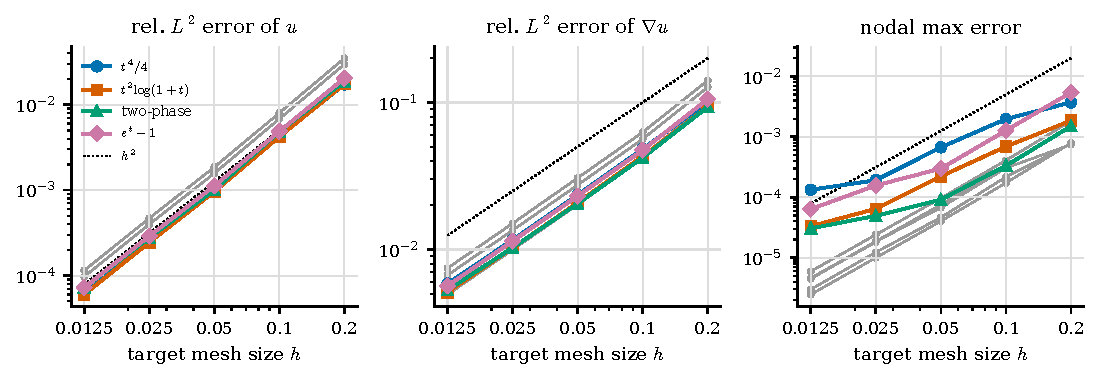
\includegraphics[width=\textwidth]{figures/F15_convergence_order.pdf}
\caption{Radial torsion on the unit disk (P1, $r=1$): relative $L^2$ errors of $u$ (left) and $\nabla u$ (center) and nodal maximum error (right) versus the mesh size. Colored: the four cases with reduced maximum-norm order ($t^4/4$, $t^2\log(1+t)$, two-phase with unresolved interface, $e^t-1$); gray: the other integrands in the top block of Table~\ref{tab:orders}; dotted: reference slopes.}\label{fig:orders}
\end{figure}

\emph{Manufactured solution.} For a nonradial test, we take $(0,1)^2$ with $G(x,t)=t^2/2+(1+x_1)t^4/4$, $u=e^{x_1+x_2}$, Dirichlet data $u$, $r=100$ and tolerance $10^{-10}$, the pairwise orders are $2.02$, $2.00$, $2.00$ ($L^2$) and $1.00$ (gradient).

\emph{The parameter $r$.} Theorem~\ref{thm:C} guarantees convergence for every $r>0$, but the speed of convergence depends strongly on $r$ (Figure~\ref{fig:r}). On the checkerboard problems of Section~\ref{ssec:lav-setting}, the iteration count varies by a factor of about $14$ (P1) to $38$ (CR) over $r\in[0.1,100]$, with the best $r$ near $1$ for CR and between $1$ and $3$ for P1, and it grows moderately under refinement at fixed $r$. For the manufactured problem ($n=40$), the counts for $r=1,10,30,100,300$ are $11\,575$, $1167$, $396$, $208$ and $516$, with $L^2$ errors that agree to four digits. For the dead core problem ($e^t-1$, $h=0.05$, tolerance $10^{-8}$), the counts for $r=1,3,10,30,100$ are $6403$, $2139$, $650$, $244$ and $529$; for $r=100$, however, the error at termination is $1.1292\times10^{-3}$, against $1.1204\times10^{-3}$ for $r\le10$. For large $r$, then, a small primal residual does not imply a small iteration error. The duality gap ($1.3\times10^{-8}$ against $2.1\times10^{-9}$) and the dual residual do flag this run, which is why we stop on both the residual and the gap.

\begin{figure}[t]
\centering
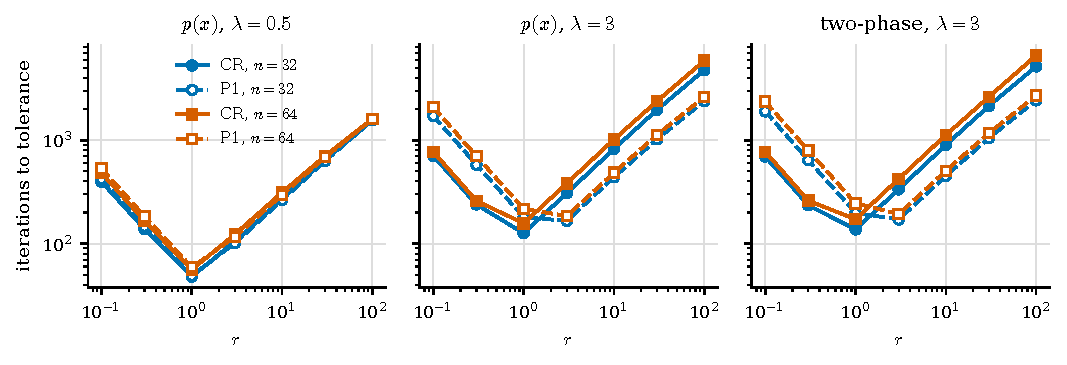
\includegraphics[width=\textwidth]{figures/F3_iterations_vs_r.pdf}
\caption{Iterations to tolerance versus the penalty parameter $r$, for CR (solid) and P1 (dashed) on criss-cross meshes with $n=32$ and $n=64$: $p(x)$ checkerboard with $\lambda=0.5$ (no gap) and $\lambda=3$, and two-phase checkerboard with $\lambda=3$ (Section~\ref{ssec:lav-setting}).}\label{fig:r}
\end{figure}

\emph{The Lyapunov functional.} Using a reference saddle point computed to residual $10^{-14}$, we checked that $E_n$ in \eqref{eq:lyap} was nonincreasing at every iteration in all runs examined: CR on the $p(x)$ checkerboard ($\lambda=3$, $n=32$, $r=1,3,10$, with $E_{100}/E_1=3\times10^{-14}$, $6\times10^{-7}$ and $8\times10^{-4}$, respectively) and P1 on the disk ($h=0.1$) for five integrands, including the nonsmooth $e^t-1$. After a transient, the decay is geometric, with rates that depend on $G$ and $r$; no rate is proved.

\subsection{(S) fails, but there is no gap}\label{ssec:roughload}
What happens when (S) fails? Example~\ref{ex:noS} can be computed: we take $p=3/2$ on the unit disk with $f=\abs x^{-\beta}$. For $\beta=1.5$, the exact solution is $4\log(1/\abs x)$, $\nabla u\notin L^2$ and (S) fails; for $\beta=1.4$, $\abs{\nabla u}\sim\abs x^{-0.8}\in L^2$ and (S) holds (Proposition~\ref{prop:S-p}(i)); for $\beta=1.6$, (S) fails again. The singular load must be integrated accurately. We use a Gauss--Jacobi rule on the triangles at the origin; the barycenter rule gives an energy error $2.5$ times larger and a far too small $\norm{\nabla u_h}$. Figure~\ref{fig:roughload} shows the diagnostics of Theorem~\ref{thm:diag}. For $\beta=1.5$, $\norm{\nabla_hu_h}^2$ grows by about $32\pi\log2\approx69.7$ per halving of $h$ (observed: $+67$, $+75$, $+61$, $+69$), consistently with $\int_{\abs x>h}\abs{\nabla u}^2=32\pi\log(1/h)$, while $\norm{\eta_h}^2\to8\pi=\norm\eta^2$ stays bounded and the iteration counts grow ($195\to589$). For $\beta=1.4$, in contrast, the increments of $\norm{\nabla_hu_h}^2$ decrease.

The P1 and CR energies approach the same limit $J(u)=-32\pi/3$, slowly ($J(u_h)-J(u)=7.58\to1.97$). P1 approaches it from above, since $u_h\in W^{1,3/2}_0$ (up to the quadrature of the singular load). Here the CR energies are also above $J(u)$. This does not contradict Theorem~\ref{thm:D}, which does not apply: $\Omega_h\neq\Omega$, $f$ is not piecewise constant, and the statement on the CR energy itself needs $f=0$. Thus a failure of (S) is visible in the iteration and in the size of the discrete saddle points, but it is not a consistency problem: P1 is adequate.

\begin{figure}[t]
\centering
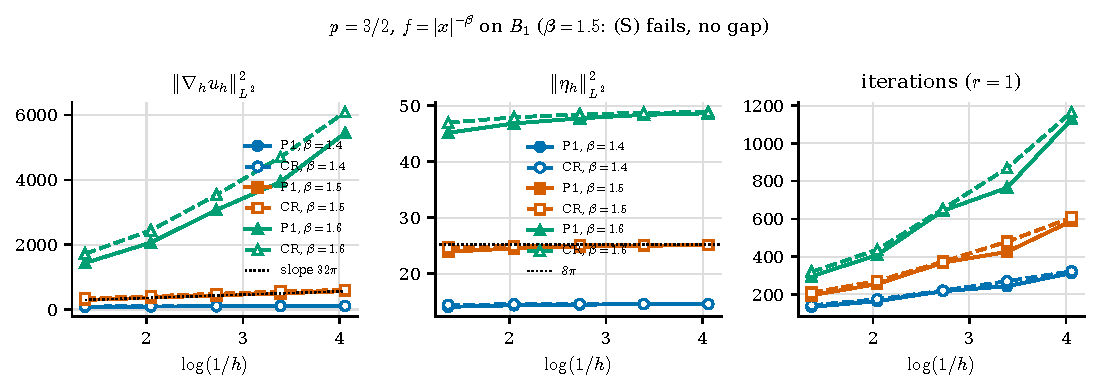
\includegraphics[width=\textwidth]{figures/F12_rough_load.pdf}
\caption{Failure of (S) without a gap: $G=t^{3/2}/(3/2)$, $f=\abs x^{-\beta}$ on the unit disk, P1 (solid) and CR (dashed), $r=1$. Squared $L^2$ norms of the discrete gradient (left) and flux (center), and iterations (right), versus $\log(1/h)$. (S) fails for $\beta=1.5,1.6$ and holds for $\beta=1.4$; dotted: slope $32\pi$ and level $8\pi$ predicted for $\beta=1.5$.}\label{fig:roughload}
\end{figure}

\subsection{The Lavrentiev experiments: setting}\label{ssec:lav-setting}
We now turn to problems with a Lavrentiev gap. We take $\Omega=(-1,1)^2$, $f=0$, and the boundary datum $\lambda u_0$, where $u_0=1$ on $\{\abs{x_1}<x_2\}$, $u_0=-1$ on $\{\abs{x_1}<-x_2\}$ and $u_0=x_2/\abs{x_1}$ elsewhere; its trace is $\lambda x_2$. The integrands are the Zhikov-type checkerboard exponent \cite{Zhikov1986}
\[
G(x,t)=t^{p(x)}/p(x),\qquad p=3\ \text{on }\{\abs{x_1}<\abs{x_2}\},\quad p=\tfrac32\ \text{elsewhere},
\]
and the two-phase checkerboard $G(x,t)=t^{3/2}/(3/2)+\mathbf 1_{\{\abs{x_1}<\abs{x_2}\}}t^3/3$. These are Experiments~1 and~3 of Balci, Ortner and Storn \cite{BalciOrtnerStorn2022}, who report, on the basis of numerical evidence, a gap for $\lambda>1$ and for $\lambda\ge0.4$, respectively. For $\lambda=1$ and the $p(x)$ problem, the minimizer is $x_2$, with energy $2$. We use criss-cross meshes ($n\times n$ squares, each cut into four triangles by its diagonals, $n=8,\dots,512$), which resolve the lines $\abs{x_1}=\abs{x_2}$, so that \eqref{eq:resolved} holds. P1 nodal data and CR edge means are exact, $r=3$, and the tolerances are $10^{-10}$ for the residual and $10^{-9}$ for the relative duality gap. All $296$ runs converged; the largest CR problem ($n=512$, $1.57\times10^6$ unknowns) took $792$ iterations.

By Proposition~\ref{prop:P1}(i), Theorem~\ref{thm:D}(ii) and Remark~\ref{rem:BOS}, all assumptions of Corollary~\ref{cor:bracket} hold: every computed P1 energy is an upper bound for $\mH$, every CR energy is a lower bound for $\mW$, and $\Delta_h\to\mH-\mW$. The certificate is exact up to round-off. The normal jumps of $\sigma_n$ never exceeded $1.1\times10^{-13}$, and $J_h(u_n)-D(\sigma_n)$ was never below $-8\times10^{-10}$ (relative $4\times10^{-11}$), so the bounds hold up to an absolute error of order $10^{-10}$. The conjugates of the two-phase integrand, which have no closed form, are evaluated as rigorous upper bounds ($s\,t_{\rm hi}-G(t_{\rm lo})$ on a verified bracket), so their evaluation does not affect the direction of the bound. For $\lambda=1$, both energies equal $2$ to within $1.5\times10^{-11}$ on every mesh.

\subsection{Brackets, widths and the signature of a gap}\label{ssec:brackets}
Figure~\ref{fig:bracket} shows the bracket for $\lambda=3$, and Table~\ref{tab:brackets} lists the finest-mesh values for a range of $\lambda$. Typical rigorous conclusions are
\[
\begin{aligned}
17.7635&\le\mW\le\mH\le18.9581&&(p(x),\ \lambda=3),\\
20.9938&\le\mW\le\mH\le23.0881&&(\text{two-phase},\ \lambda=3),
\end{aligned}
\]
so that the gap is at most $1.195$ and $2.094$, respectively. At the other end of the range, the gap is at most $8.0\times10^{-7}$ for $p(x)$ with $\lambda=0.5$, and at most $2.5\times10^{-8}$ for the two-phase problem with $\lambda=0.2$. These numbers certify the (near) absence of a gap; the positivity of a gap, as explained in Remark~\ref{rem:gap-indicator}(c), cannot be certified.

\begin{figure}[t]
\centering
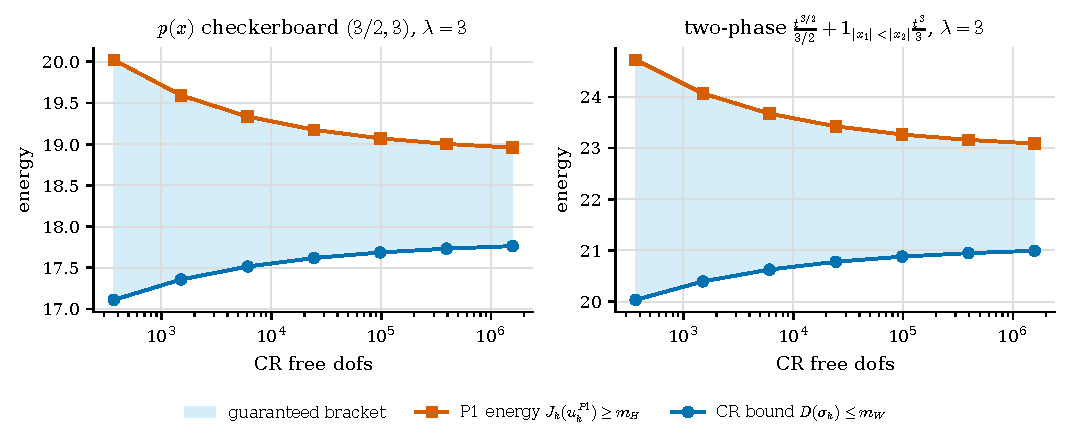
\includegraphics[width=\textwidth]{figures/F1_bracket_lambda3.pdf}
\caption{Guaranteed brackets $D(\sigma_h)\le\mW\le\mH\le J_h(u_h^{\Pone})$ (shaded) versus the number of CR unknowns, for the $p(x)$ (left) and two-phase (right) checkerboards with boundary datum $3u_0$. Upper curve: P1 energy; lower curve: CR energy $=D(\sigma_h)$.}\label{fig:bracket}
\end{figure}

\begin{table}[t]
\caption{Finest-mesh brackets for the checkerboard problems: P1 energy ($\ge\mH$), certified lower bound $D(\sigma_n)$ ($\le\mW$), width $\Delta_h\ge\mH-\mW$, ratio $\Delta_{n/2}/\Delta_n$ on the two finest meshes, and slope of $\Delta_h$ versus the number of unknowns (four finest meshes). Ratio $4$, slope $-1$: $O(h^2)$ closure.}\label{tab:brackets}
\small
\begin{tabular}{@{}lrrcccc@{}}
\toprule
problem, $\lambda$ & $n$ & P1 energy & lower bound $D$ & width $\Delta_h$ & ratio & slope\\
\midrule
$p(x)$, $0.5$ & 512 & 0.51381346 & 0.51381265 & $8.0\times10^{-7}$ & 4.00 & $-1.00$\\
$p(x)$, $1$ & 256 & 2.00000000 & 2.00000000 & $\le1.5\times10^{-11}$ & -- & --\\
$p(x)$, $1.08$ & 256 & 2.33326877 & 2.33325614 & $1.3\times10^{-5}$ & 2.02 & $-0.53$\\
$p(x)$, $1.5$ & 256 & 4.52197423 & 4.51556823 & $6.4\times10^{-3}$ & 1.31 & $-0.24$\\
$p(x)$, $2$ & 256 & 8.12513230 & 8.02915903 & $9.6\times10^{-2}$ & 1.17 & $-0.15$\\
$p(x)$, $3$ & 512 & 18.95812228 & 17.76348924 & 1.195 & 1.06 & $-0.06$\\
$p(x)$, $4$ & 256 & 35.76099252 & 30.51017011 & 5.251 & 1.07 & $-0.06$\\
\midrule
two-phase, $0.2$ & 512 & 0.24363748 & 0.24363745 & $2.5\times10^{-8}$ & 3.23 & $-0.84$\\
two-phase, $0.4$ & 256 & 0.71309620 & 0.71309059 & $5.6\times10^{-6}$ & 2.45 & $-0.67$\\
two-phase, $1$ & 256 & 3.15984497 & 3.15462093 & $5.2\times10^{-3}$ & 1.34 & $-0.26$\\
two-phase, $3$ & 512 & 23.08812916 & 20.99380420 & 2.094 & 1.06 & $-0.06$\\
two-phase, $4$ & 256 & 41.75864138 & 34.43734359 & 7.321 & 1.06 & $-0.06$\\
\bottomrule
\end{tabular}
\end{table}

Figure~\ref{fig:width} shows $\Delta_h$ versus the number of unknowns for all values of $\lambda$, and two regimes are clearly separated. For small $\lambda$ the width closes at a steady rate. For large $\lambda$, in contrast, the closure ratio per refinement decreases towards $1$ ($1.30$, $1.23$, $1.17$, $1.12$, $1.09$, $1.06$ for $p(x)$ with $\lambda=3$), that is, the width stalls. Since $\Delta_h$ converges to the gap by Corollary~\ref{cor:bracket}, a width that stalls at a value of order $1$ is the signature of a gap, although it is not a proof of one. Heuristic extrapolations (Aitken's method, or least-squares fits with a free exponent over the three or four finest meshes) give closure exponents $\approx0.56$--$0.60$ in $h$ that \emph{decrease} with refinement. The free-exponent fits give estimated gaps of about $1.04$ ($p(x)$, $\lambda=3$) and $1.85$ (two-phase, $\lambda=3$), and fixed exponents $1$ or $2$ would give up to $1.17$ and $2.06$. Because the fitted exponent keeps drifting, we regard these numbers only as conjectural; the rigorous statement is the bracket.

\begin{figure}[t]
\centering
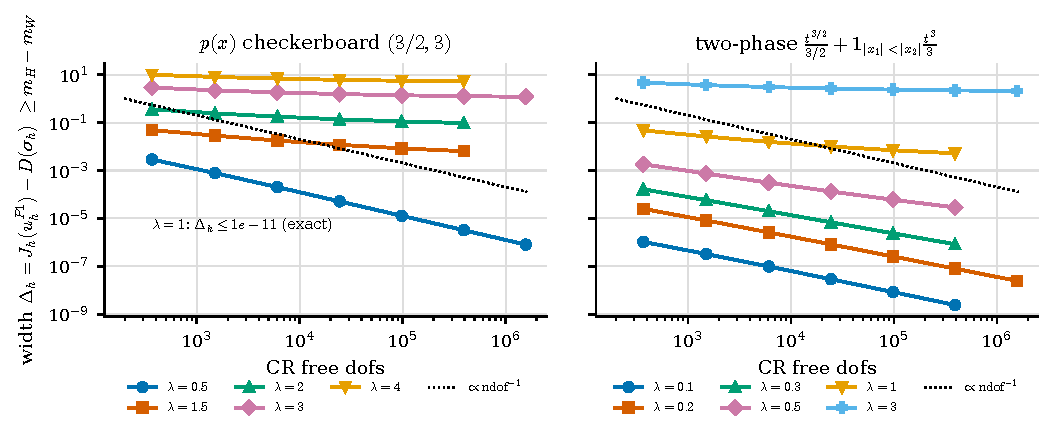
\includegraphics[width=\textwidth]{figures/F2_width_vs_ndof.pdf}
\caption{Width $\Delta_h=J_h(u_h^{\Pone})-D(\sigma_h)\ge\mH-\mW$ of the guaranteed bracket versus the number of CR unknowns, for the $p(x)$ (left) and two-phase (right) checkerboards and several data $\lambda u_0$. Dotted: slope $\mathrm{ndof}^{-1}$, i.e.\ $O(h^2)$. For $p(x)$ with $\lambda=1$ the width is at round-off level.}\label{fig:width}
\end{figure}

\emph{No-gap controls, and a first surprise.} For the $p(x)$ problem with $\lambda\in\{0.25,0.5\}$, the ratios tend to $4.00$ (slope $-1.00$): both bounds close at $O(h^2)$, as expected without a gap (compare the $O(\mathrm{ndof}^{-1})$ reported in \cite[Exp.~1]{BalciOrtnerStorn2022}); for $\lambda=0.75$, the ratios ($3.0\to3.84$) are still pre-asymptotic. For the two-phase problem with $\lambda\in\{0.1,0.2\}$, however, the ratios are only $3.2$--$3.5$ (slope $\approx-0.85$), also on $n=512$, and both bounds close at the same reduced rate. We expected $4$ and have no explanation. The effect is not caused by the solver: the final discrete duality gaps of these runs are below $3\times10^{-12}$, four orders of magnitude below the widths, which are themselves below $2.5\times10^{-8}$. The rate of closure alone, therefore, does not separate gap from no gap; in all our runs its trend under refinement did (an observation, not a theorem).


\emph{Near the thresholds, a second surprise.} The computations of \cite{BalciOrtnerStorn2022} indicate a gap for $p(x)$ with $\lambda>1$ and for the two-phase problem with $\lambda\ge0.4$. Our widths for $\lambda\in(1,1.08]$ ($p(x)$) and $\lambda\in\{0.4,0.5,0.6\}$ (two-phase), however, still decrease steadily on uniform meshes up to $n=256$, with ratios $2.0$--$2.5$ that decline only slowly, so they neither confirm nor exclude a gap there. Rigorously, the gap is at most $1.3\times10^{-5}$ for $p(x)$ with $\lambda=1.08$, and at most $1.2\times10^{-4}$ for the two-phase problem with $\lambda=0.6$.

Figure~\ref{fig:bos} compares our widths with the differences $F(u_c)-F_h(u_{nc})$ of \cite[Fig.~1]{BalciOrtnerStorn2022}, which we read from the vector graphics, identifying the color of each curve from the legend samples. Their adaptive meshes reach values $10$--$100$ times smaller than our uniform meshes. Since their initial meshes resolve the exponent, their conforming energies are exact and their CR energies have $f=0$, Proposition~\ref{prop:P1} and Theorem~\ref{thm:D} make their differences upper bounds for the gap as well, provided their discrete CR problems are solved accurately. Read in this way, their data bound the gap at $\lambda=1.08$ by about $4\times10^{-7}$ (observed). Neither data set shows a plateau for $\lambda\le1.08$. In both, however, the closure rate \emph{decreases} under refinement for $\lambda\ge1.04$ (our ratios $2.28\to2.21$, $2.24\to2.11$, $2.21\to2.02$; their slope for $\lambda=1.08$ drops from about $-1.1$ to $-0.45$), whereas it is steady or increasing for $\lambda=0.99$; this is the pattern of the gap cases. Since $\mH-\mW$ vanishes at $\lambda=1$, a gap below the final widths is compatible with all the data. We conclude only that the gap for $\lambda\in(1,1.08]$, if present, is below $1.3\times10^{-5}$ (our bound) and plausibly below $4\times10^{-7}$; it cannot be certified either way. The widths stall, which is the signature of a gap but not a proof of one (Remark~\ref{rem:gap-indicator}(c)), for $\lambda\ge1.5$ ($p(x)$) and $\lambda\ge1$ (two-phase).

\begin{figure}[t]
\centering
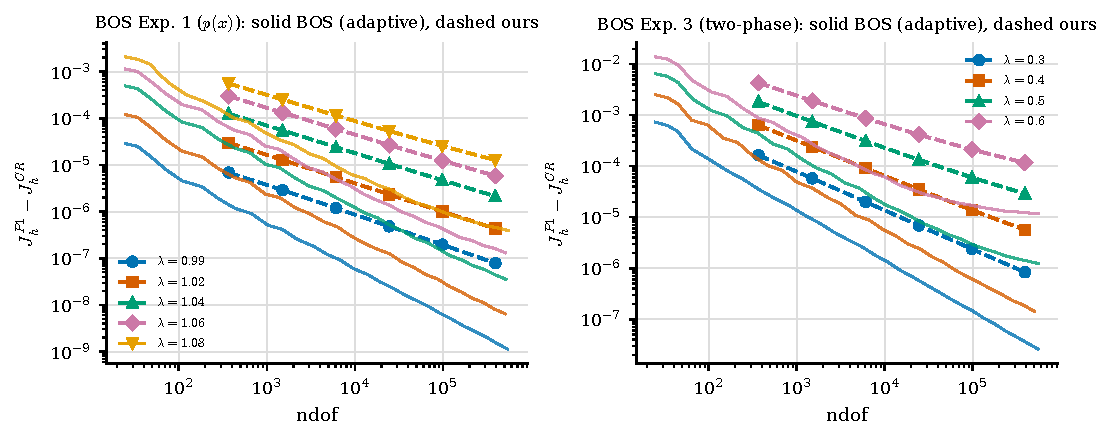
\includegraphics[width=\textwidth]{figures/F6c_bos_overlay.pdf}
\caption{Near the gap thresholds reported in \cite{BalciOrtnerStorn2022}: our certified widths $J_h^{\Pone}-D(\sigma_n)$ (uniform meshes; dashed, markers) and the differences digitized from \cite[Fig.~1]{BalciOrtnerStorn2022} (adaptive meshes; solid) versus the number of unknowns. Left: $p(x)$ checkerboard, $\lambda=0.99,\dots,1.08$; right: two-phase checkerboard, $\lambda=0.3,\dots,0.6$. Our widths equal $J_h^{\Pone}-J_h^{\CR}$ to within $3\times10^{-12}$.}\label{fig:bos}
\end{figure}

\emph{Quadrature.} The guarantees depend on how the coefficients are sampled. Reproducing \cite[\S4.2]{BalciOrtnerStorn2022} ($p(x)$, $\lambda=5$), we find that replacing the exponent on the nodal patch of the origin by its maximum sends \emph{both} P1 and CR towards the P1 value ($59.73$ for exact sampling on $n=256$; perturbed: P1 $60.66$, CR $59.91$), and replacing it by its minimum sends both towards the CR value ($45.93$; perturbed: $45.85$, $45.52$). The perturbed energies are not bounds for the original problem: the guarantees of Proposition~\ref{prop:P1} and Theorem~\ref{thm:D} require a majorant sampling for P1 and a minorant sampling for CR (Remark~\ref{rem:gap-indicator}(d)).

\subsection{The size of the discrete saddle points}\label{ssec:diag-num}
The second diagnostic is the size of the discrete saddle points. Figure~\ref{fig:diag} shows the quantities of Theorem~\ref{thm:diag}. In the gap regime, $\max\abs{\eta_h^{\Pone}}$ grows like $h^{-0.9}$ (e.g.\ $104.8\to367.4\to706.4$ for $p(x)$, $\lambda=3$, $n=64,256,512$, and $138\to492\to951$ for the two-phase problem), consistently with Theorem~\ref{thm:diag}(d); recall that the gap for these data is inferred, not proved. The CR flux grows much more slowly ($11.9\to22.7\to31.6$). A flux that grows like $h^{-0.9}$ at a single point is consistent with a singularity $\abs{\eta}\sim\abs x^{-0.9}$, which lies in $L^2$, so this growth says nothing against (S). Growth of $\max\abs{\eta_h}$ alone is not a gap indicator either: it grows mildly also without a gap ($0.54\to0.57\to0.59$ for the two-phase problem with $\lambda=0.2$). The observed rates differ by an order of magnitude, but we have no theory for them.

The $L^2$ norms behave differently. The CR gradient norm $\norm{\nabla_hu_h^{\CR}}$ increases slowly ($7.57\to7.73\to7.82$), roughly like $(\log(1/h))^{1/2}$, which is consistent with, but does not establish, an unbounded CR family. The P1 norms $\norm{\nabla u_h}$ ($6.565\to6.612\to6.627$) and $\norm{\eta_h}$ ($9.145\to9.158\to9.212$) look bounded up to $n=512$, except for the last increment of $\norm{\eta_h}$. By Theorem~\ref{thm:diag}(a), bounded P1 saddle points would imply (S) together with $\mH=\mHone$; if the gap inferred above is real, this would be an instance of (S) \emph{with} a gap, in line with the discussion after Proposition~\ref{prop:twophase}. The data are too short to decide.

\begin{figure}[t]
\centering
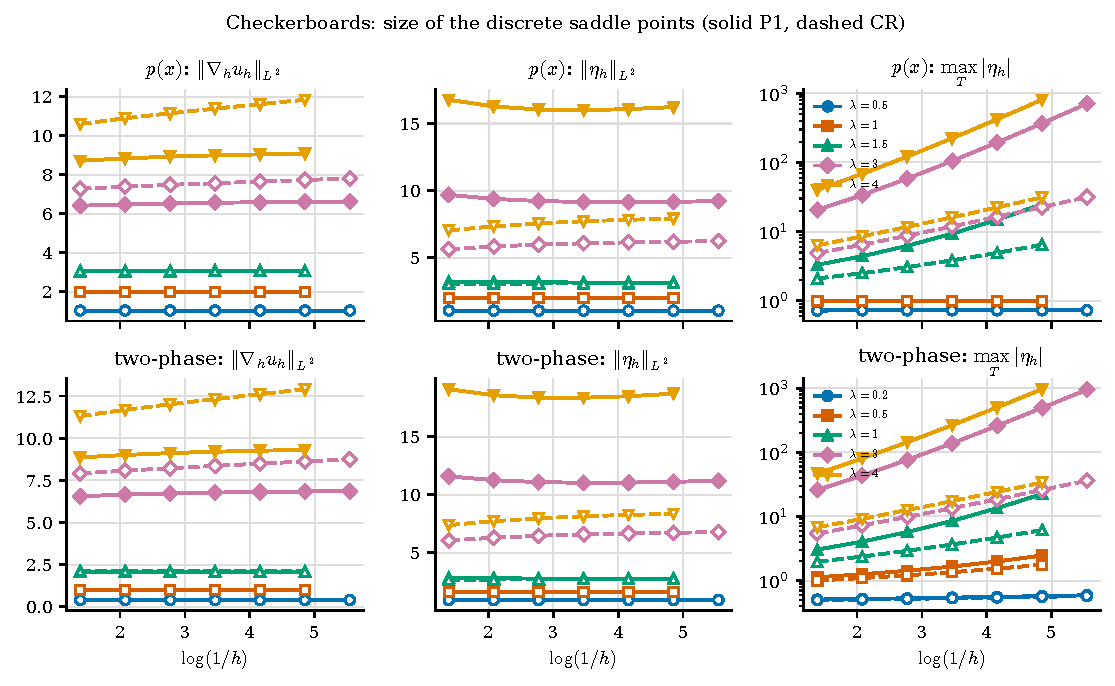
\includegraphics[width=\textwidth]{figures/F7b_diagnostics_checkerboard.pdf}
\caption{Size of the discrete saddle points for the $p(x)$ (top) and two-phase (bottom) checkerboards, P1 (solid) and CR (dashed), several data $\lambda u_0$, versus $\log(1/h)$: $\norm{\nabla_hu_h}_{L^2}$ (left), $\norm{\eta_h}_{L^2}$ (center) and $\max_T\abs{\eta_h}$ (right, logarithmic scale).}\label{fig:diag}
\end{figure}

\subsection{Beyond the checkerboards}\label{ssec:beyond}
The checkerboards have piecewise constant coefficients and polynomial growth. Two further examples test what happens when either property is lost.

\emph{Double phase with the Esposito--Leonetti--Mingione weight.} Let $G=t^{1.5}/1.5+a(x)t^q/q$ with $a=\max(x_2^2-x_1^2,0)/\abs x$, which is Lipschitz (so $\alpha=1$), data $\lambda u_0$ and $f=0$. The no-gap range of \cite[Thm.~2.3]{BGS2022} is then $q\le2.5$, while $q=4>d+\alpha$ lies in the range of the counterexamples of \cite{ELM2004}. Since $a$ is not piecewise constant, a rigorous bracket is obtained from a majorant sampling for P1 and a minorant sampling for CR (Remarks~\ref{rem:Lip-smooth}(c) and~\ref{rem:gap-indicator}(d)). Its width, however, is dominated by the $O(h)$ sampling error: the bracket is, for example, $[82.15,82.85]$ for $q=2.4$, $\lambda=8$, $n=256$, and $[101.6,196.6]$ for $q=4$, $\lambda=8$ (gap $\le95.0$). The difference of the barycenter-sampled P1 and CR energies, for which we have no theory, is more informative. For $q=2.4$ it closes at $O(h^2)$ (ratio $\to4$) for all $\lambda\le8$. For $q=4$ it stalls for $\lambda\ge4$ (ratios $1.59\to1.30$ for $\lambda=4$), while $\max\abs{\eta_h^{\Pone}}$ grows; it is ambiguous at $\lambda=2$ (steady ratio $\approx2.45$) and closes at $O(h^2)$ for $\lambda\le1$. For $q=2.8$ and $\lambda=8$ it closes at a ratio $2.4$--$2.6$ that increases with $n$, so the case remains undecided for $n\le128$.

\emph{An exponential checkerboard.} The integrand $G=a(x)(e^t-1-t)+t^2/2$ with $a=\mathbf 1_{\{\abs{x_1}<\abs{x_2}\}}$ satisfies neither the growth condition of \cite{BalciOrtnerStorn2022} nor $\Delta_2$, but Theorem~\ref{thm:D} still applies. At $n=256$ the bracket is $[0.740687,0.740812]$ for $\lambda=0.5$ and $[35.18,37.45]$ for $\lambda=3$, and the width stalls for $\lambda\ge2$ (ratio $1.13$ at $\lambda=3$), the pattern of the gap cases above. We know of no theory for the gap in this problem.

\subsection{Discussion}\label{ssec:discussion}
The experiments confirm the division of labor suggested by the theory. The solver is never the problem: the iteration converged in every Lavrentiev run, for every $r$, as Theorem~\ref{thm:C} guarantees, and a failure of (S) showed up only as iteration counts growing under refinement (observed for one example, Section~\ref{ssec:roughload}). What a gap changes is the meaning of the computed numbers. Here the bracket of Corollary~\ref{cor:bracket} turns two schemes that converge separately, but to different targets, into a computable statement about $\mW$ and $\mH$. Three observations did not match our expectations, and we report them as such. The no-gap two-phase controls close at a ratio $3.2$--$3.5$ rather than $4$; near the reported thresholds, neither data set shows a plateau, although both show a decreasing closure rate; and the P1 saddle points in the gap regime look bounded in $L^2$ up to $n=512$, which, if both this boundedness and the gap are real, would be an instance of (S) with a gap. Finally, we recall the limitations of the experiments: widths certify upper bounds only, extrapolations are heuristic, and the disk errors are computed on inscribed polygons against radial solutions computed by quadrature.

%======================================================================
\section{Conclusions and open problems}\label{sec:conclusions}
For an arbitrary convex Young integrand and $\rho=r$, the convergence of Glowinski's method at the continuous level is equivalent to the boundedness of the iterates, and it hinges on the regularity assumption (S). Under (S), the iteration converges weakly in general and strongly under Lieberman's condition, without any continuity in $x$. Assumption~(S), however, is not available in general for double phase, two-phase and exponential energies, and it is a different property from the absence of a Lavrentiev gap. At the discrete level, the iteration converges unconditionally, for P1 and CR alike, and the remaining issue is consistency, which is governed by the gap. Under the assumptions of \cite[Thm.~1]{BalciOrtnerStorn2022} (polynomial growth, resolved or minimum quadrature), CR elements give the method a convergence theory in the Lavrentiev regime (Theorem~\ref{thm:C} and \cite[Thm.~1]{BalciOrtnerStorn2022}). Moreover, the CR iterates carry a guaranteed lower bound for $\mW$, which, together with the P1 energy, brackets the gap.

Several problems remain open. (1) The behavior of $u_n$ when (S) fails, in which case $(\eta_n,\nu_n)$ is unbounded; cf.\ \cite[Rem.~23]{GlowinskiPanTai2016}. (2) Strong convergence of $u_n$ for general convex $G$, the case $\rho\ne r$ without Glowinski's hypotheses (iii)--(iv), and rates for the iteration, including their dependence on $h$ and $r$ and a theory for the choice of $r$. (3) Whether (S) can hold together with a gap for loads $f\in L^d$; Example~\ref{ex:Sgap} is degenerate, and the P1 data of Section~\ref{ssec:diag-num} are suggestive but not conclusive. (4) A computable \emph{lower} bound for $\mH$, which would certify the positivity of a gap. (5) Rates for the width $\Delta_h$, an explanation of the observed $O(h^2)$ closure without a gap and of its reduced rate for the two-phase controls, and an extension of Theorem~\ref{thm:D} to $f\neq0$ for the CR energy itself and to non-resolved coefficients with sampling errors smaller than $O(h)$. (6) Global regularity, and hence (S), for Musielak--Orlicz integrands $G(x,t)$ without $\Delta_2$ and for double phase energies up to the boundary.

\subsection*{Software availability}
The Python package \texttt{glaplace} (NumPy/SciPy; MIT license) implements the method with P1 and CR elements for arbitrary Young functions on two-dimensional triangulations, including the certified lower bound of Theorem~\ref{thm:D}. It contains the scripts and raw data of all experiments of Section~\ref{sec:numerics} and is available at \url{https://github.com/jfbonder/glaplace}. It generalizes the code for the $p(x)$-Laplacian of \cite{AragonFBRubio2023}.

\subsection*{Declaration of the use of AI tools}
Generative AI was used extensively in this work, in the form of Claude models developed by Anthropic, accessed through the Claude desktop application and its agent tools (October 2026). The research problem, the choice of the method and of the test problems, and the scientific direction are the authors'. The AI tools were used for the following tasks: (i) writing the Python code of the solver and of all numerical experiments, including the tests, starting from the authors' original MATLAB code for the $p(x)$-Laplacian (the code of \cite{AragonFBRubio2023}), which was translated to Python and extended to general Young functions and to Crouzeix--Raviart elements; (ii) drafting the proofs of Theorems~\ref{thm:A}--\ref{thm:D} and of the auxiliary results, starting from the authors' earlier unpublished argument at the continuous level; (iii) searching and compiling the literature, extracting the hypotheses of the cited results from the sources, and checking the bibliographic data; (iv) drafting and editing the text of the article; (v) independent critical reviews of the mathematics and of the exposition, carried out by separate instances of the model; and (vi) in the final rewriting, a team of AI agents with separate roles (numerical analyst, expert in nonlinear partial differential equations, programmer, bibliography reviewer, editor and translator), whose drafts, computations and reports were checked against each other, followed by two further independent referee reports by AI agents (numerical analysis and PDE), whose recommendations were incorporated into the text.
 The numerical results reported here were produced by running the code described above. The authors take full responsibility for the content of the article. % TODO (authors): provisional; update after the authors' full revision and according to the requirements of the target journal.

\subsection*{Acknowledgements}
% TODO: funding information.
TODO: funding.

% Bibliography: reports/bibliography_v4.tex (bibliography reviewer), restricted to cited entries; status comments kept.
\begin{thebibliography}{99}
\setlength{\itemsep}{0pt}

\bibitem{AcerbiMingione2001}
E.~Acerbi and G.~Mingione, \emph{Regularity results for a class of functionals with non-standard growth}, Arch. Ration. Mech. Anal. \textbf{156} (2001), no.~2, 121--140.
% VERIFIED (SEC: refs of arXiv:2303.10687, 2601.11495). DOI (memory) 10.1007/s002050100117.

\bibitem{AcerbiMingione2002}
E.~Acerbi and G.~Mingione, \emph{Regularity results for stationary electro-rheological fluids}, Arch. Ration. Mech. Anal. \textbf{164} (2002), no.~3, 213--259.
% CORRECTED (issue no. 3 added; SEC). NB: the PDF in biblio/ (CRMATH_2002__334_9_817_0.pdf) is a DIFFERENT paper:
% E. Acerbi, G. Mingione, "Regularity results for electrorheological fluids: the stationary case",
% C. R. Math. Acad. Sci. Paris 334 (2002), no. 9, 817--822 [VERIFIED (PDF)]; cite that one only if intended.

\bibitem{Antonini2026}
C.~A. Antonini, \emph{Local and global $C^{1,\beta}$-regularity for uniformly elliptic quasilinear equations of $p$-Laplace and Orlicz-Laplace type}, preprint, arXiv:2601.07140v3 (2026).
% CORRECTED: title/author VERIFIED (PDF, v3 dated 27 Aug 2026); the journal "Nonlinear Anal. (2026)" could not be
% verified and was removed. If the authors confirm publication, add volume/article number and DOI.

\bibitem{AragonFBRubio2023}
A.~Arag\'on, J.~Fern\'andez Bonder and D.~Rubio, \emph{Effective numerical computation of $p(x)$-Laplace equations in 2D}, Int. J. Comput. Math. \textbf{100} (2023), no.~11, 2111--2123; arXiv:2204.08054.
% Title/authors VERIFIED (PDF arXiv v2); journal/volume/pages NOT-CHECKABLE from the folder (authors' own paper: check).

\bibitem{ArnoldBrezzi1985}
D.~N. Arnold and F.~Brezzi, \emph{Mixed and nonconforming finite element methods: implementation, postprocessing and error estimates}, RAIRO Mod\'el. Math. Anal. Num\'er. \textbf{19} (1985), no.~1, 7--32.
% FROM-MEMORY (new). Check vol/issue/pages; DOI (memory) 10.1051/m2an/1985190100071.

\bibitem{BalciKaltenbach2023}
A.~Kh. Balci and A.~Kaltenbach, \emph{Error analysis for a Crouzeix--Raviart approximation of the variable exponent Dirichlet problem}, preprint, arXiv:2303.10687v4 (2024).
% VERIFIED (PDF, v4 of 22 Apr 2024). Published version not identified: author must check (journal, vol., pages).

\bibitem{BDS2020}
A.~Kh. Balci, L.~Diening and M.~Surnachev, \emph{New examples on Lavrentiev gap using fractals}, Calc. Var. Partial Differential Equations \textbf{59} (2020), no.~5, Paper No.~180, 34~pp.; doi:10.1007/s00526-020-01818-1; arXiv:1906.04639.
% VERIFIED (SEC: refs of 2106.06837 [BDS20] with DOI, 2110.13945, 2303.05877). Theorem numbers used in the text are those of arXiv v2.

\bibitem{BalciOrtnerStorn2022}
A.~Kh. Balci, C.~Ortner and J.~Storn, \emph{Crouzeix--Raviart finite element method for non-autonomous variational problems with Lavrentiev gap}, Numer. Math. \textbf{151} (2022), no.~4, 779--805; doi:10.1007/s00211-022-01303-1; arXiv:2106.06837.
% VERIFIED (title PDF arXiv v1; journal data SEC: refs of 2303.10687 [7]). Section/theorem numbers checked in arXiv v1.

\bibitem{BaroniColomboMingione2018}
P.~Baroni, M.~Colombo and G.~Mingione, \emph{Regularity for general functionals with double phase}, Calc. Var. Partial Differential Equations \textbf{57} (2018), no.~2, Art.~62, 48~pp.; doi:10.1007/s00526-018-1332-z; arXiv:1708.09147.
% VERIFIED (title PDF arXiv v1; journal SEC: refs of 2303.05877, 2601.07140 with DOI). Thm numbers checked in arXiv v1.

\bibitem{BarrettLiu1993}
J.~W. Barrett and W.~B. Liu, \emph{Finite element approximation of the $p$-Laplacian}, Math. Comp. \textbf{61} (1993), no.~204, 523--537; doi:10.1090/S0025-5718-1993-1192966-4.
% VERIFIED (PDF first page; DOI = file name of the AMS PDF).

\bibitem{Bartels2021}
S.~Bartels, \emph{Nonconforming discretizations of convex minimization problems and precise relations to mixed methods}, Comput. Math. Appl. \textbf{93} (2021), 214--229; doi:10.1016/j.camwa.2021.04.014.
% VERIFIED (SEC: refs of 2106.06837 [Bar21] and 2303.10687 [10]) (new; CR--RT0 discrete duality, one-point quadrature).
% CHECK (authors): content (CR/RT0 duality, CR lower energy bounds) cited FROM-MEMORY of the NA referee; paper not read by the team.

\bibitem{BartelsMilicevic2017}
S.~Bartels and M.~Milicevic, \emph{Alternating direction method of multipliers with variable step sizes}, preprint, arXiv:1704.06069 (2017).
% VERIFIED (PDF arXiv v1). Journal version not identified (author: check).

\bibitem{BauschkeCombettes2017}
H.~H. Bauschke and P.~L. Combettes, \emph{Convex Analysis and Monotone Operator Theory in Hilbert Spaces}, 2nd ed., CMS Books in Mathematics, Springer, Cham, 2017.
% FROM-MEMORY (no PDF). Standard; DOI (memory) 10.1007/978-3-319-48311-5.

\bibitem{BCDM2024}
M.~Borowski, I.~Chlebicka, F.~De Filippis and B.~Miasojedow, \emph{Absence and presence of Lavrentiev's phenomenon for double phase functionals upon every choice of exponents}, Calc. Var. Partial Differential Equations \textbf{63} (2024), Art.~35; arXiv:2303.05877.
% Title/authors VERIFIED (PDF arXiv v1); journal/vol/article NOT-CHECKABLE (check).

\bibitem{Boyd2011ADMM}
S.~Boyd, N.~Parikh, E.~Chu, B.~Peleato and J.~Eckstein, \emph{Distributed optimization and statistical learning via the alternating direction method of multipliers}, Found. Trends Mach. Learn. \textbf{3} (2011), no.~1, 1--122; doi:10.1561/2200000016.
% VERIFIED (PDF first page: "Vol. 3, No. 1 (2010) 1-122, (c) 2011", DOI printed). Year 2011 is the usual citation.

\bibitem{BreitDieningSchwarzacher2015}
D.~Breit, L.~Diening and S.~Schwarzacher, \emph{Finite element approximation of the $p(\cdot)$-Laplacian}, SIAM J. Numer. Anal. \textbf{53} (2015), no.~1, 551--572; doi:10.1137/130946046; arXiv:1311.5121.
% VERIFIED (title PDF; journal SEC: refs of 2106.06837, 2303.10687 with DOI).

\bibitem{BuffaOrtner2009}
A.~Buffa and C.~Ortner, \emph{Compact embeddings of broken Sobolev spaces and applications}, IMA J. Numer. Anal. \textbf{29} (2009), no.~4, 827--855; doi:10.1093/imanum/drn038.
% VERIFIED (SEC: refs of 2106.06837 [BO09], 2303.10687 [18]) (new; discrete Poincare/compactness in broken W^{1,p}).

\bibitem{BuiCombettes2020}
M.~N. B\`ui and P.~L. Combettes, \emph{The Douglas--Rachford algorithm converges only weakly}, SIAM J. Control Optim. \textbf{58} (2020), no.~2, 1118--1120; arXiv:1912.09564.
% Title/authors VERIFIED (PDF arXiv v1); vol/issue/pages FROM-MEMORY (check).

\bibitem{BGS2022}
M.~Bul\'i\v{c}ek, P.~Gwiazda and J.~Skrzeczkowski, \emph{On a range of exponents for absence of Lavrentiev phenomenon for double phase functionals}, Arch. Ration. Mech. Anal. \textbf{246} (2022), no.~1, 209--240; arXiv:2110.13945.
% VERIFIED (title PDF arXiv v1; journal SEC: refs of 2303.05877 [11]). Issue no. 1 added. DOI not verified.

\bibitem{CarstensenLiu2015}
C.~Carstensen and D.~J. Liu, \emph{Nonconforming FEMs for an optimal design problem}, SIAM J. Numer. Anal. \textbf{53} (2015), no.~2, 874--894; doi:10.1137/130927103.
% VERIFIED except issue no. (SEC: refs of 2106.06837 [CL15]; issue no. 2 FROM-MEMORY) (new; CR lower energy bounds).
% CHECK (authors): content (CR/RT0 duality, CR lower energy bounds) cited FROM-MEMORY of the NA referee; paper not read by the team.

\bibitem{CarstensenOrtner2010}
C.~Carstensen and C.~Ortner, \emph{Analysis of a class of penalty methods for computing singular minimizers}, Comput. Methods Appl. Math. \textbf{10} (2010), no.~2, 137--163; doi:10.2478/cmam-2010-0008.
% VERIFIED (PDF first page; DOI SEC: refs of 2106.06837 [CO10]).

\bibitem{CianchiMazya2011}
A.~Cianchi and V.~G. Maz'ya, \emph{Global Lipschitz regularity for a class of quasilinear elliptic equations}, Comm. Partial Differential Equations \textbf{36} (2011), no.~1, 100--133; doi:10.1080/03605301003657843.
% VERIFIED (SEC: refs of 2601.07140 [33] with DOI, 2206.15330, 1703.07446). No PDF.

\bibitem{CianchiMazya2014JEMS}
A.~Cianchi and V.~G. Maz'ya, \emph{Gradient regularity via rearrangements for $p$-Laplacian type elliptic boundary value problems}, J. Eur. Math. Soc. (JEMS) \textbf{16} (2014), no.~3, 571--595; doi:10.4171/JEMS/440.
% VERIFIED (title PDF preprint 12-07-2011; journal SEC: refs of 2601.07140 [35]). Thm numbers checked in the preprint only.

\bibitem{CianchiMazya2018}
A.~Cianchi and V.~G. Maz'ya, \emph{Second-order two-sided estimates in nonlinear elliptic problems}, Arch. Ration. Mech. Anal. \textbf{229} (2018), no.~2, 569--599; doi:10.1007/s00205-018-1223-7; arXiv:1703.07446.
% VERIFIED (SEC: refs of 2210.06402 [CM18] with DOI; 2007.07469 [23]). NB arXiv v1 title differs:
% "Second-order L^2-regularity in nonlinear elliptic problems". Thm 2.3/Rems 2.6-2.8 checked in arXiv v1.

\bibitem{ColomboMingione2015a}
M.~Colombo and G.~Mingione, \emph{Regularity for double phase variational problems}, Arch. Ration. Mech. Anal. \textbf{215} (2015), no.~2, 443--496; doi:10.1007/s00205-014-0785-2.
% VERIFIED (PDF published version colombo2014.pdf: volume, pages, DOI).

\bibitem{ColomboMingione2015b}
M.~Colombo and G.~Mingione, \emph{Bounded minimisers of double phase variational integrals}, Arch. Ration. Mech. Anal. \textbf{218} (2015), no.~1, 219--273; doi:10.1007/s00205-015-0859-9.
% VERIFIED (PDF colombo2015.pdf: title, DOI; vol/pages SEC: refs of 2106.06837 [CM15]).

\bibitem{CosciaMingione1999}
A.~Coscia and G.~Mingione, \emph{H\"older continuity of the gradient of $p(x)$-harmonic mappings}, C. R. Acad. Sci. Paris S\'er. I Math. \textbf{328} (1999), no.~4, 363--368.
% VERIFIED (SEC: several refs, e.g. 1708.09147, 1902.00261).

\bibitem{CrouzeixRaviart1973}
M.~Crouzeix and P.-A. Raviart, \emph{Conforming and nonconforming finite element methods for solving the stationary Stokes equations.~I}, Rev. Fran\c{c}aise Automat. Informat. Recherche Op\'erationnelle S\'er. Rouge \textbf{7} (1973), no.~R-3, 33--75.
% VERIFIED (SEC: refs of 2303.10687 [23] and Ortner 2011 [12]) (new). DOI (memory) 10.1051/m2an/197307R300331.

\bibitem{DeFilippisMingione2021}
C.~De Filippis and G.~Mingione, \emph{Lipschitz bounds and nonautonomous integrals}, Arch. Ration. Mech. Anal. \textbf{242} (2021), 973--1057; doi:10.1007/s00205-021-01698-5; arXiv:2007.07469.
% VERIFIED (DOI printed on arXiv v2; vol/pages SEC: refs of 2601.11495 [25]).

\bibitem{DelPezzoMartinez2015}
L.~M. Del Pezzo and S.~Mart\'inez, \emph{Order of convergence of the finite element method for the $p(x)$-Laplacian}, IMA J. Numer. Anal. \textbf{35} (2015), no.~4, 1864--1887; arXiv:1311.3230.
% VERIFIED (title PDF arXiv v2; journal SEC: refs of 2204.08054 [7]).

\bibitem{DHHR2011}
L.~Diening, P.~Harjulehto, P.~H\"ast\"o and M.~R\r{u}\v{z}i\v{c}ka, \emph{Lebesgue and Sobolev Spaces with Variable Exponents}, Lecture Notes in Mathematics~2017, Springer, Heidelberg, 2011; doi:10.1007/978-3-642-18363-8.
% VERIFIED (SEC: refs of 2303.10687 [27], 1906.04639 [5]) (new; Sect. 4.6 = density of smooth functions under log-Hoelder).

\bibitem{DiBenedetto1983}
E.~DiBenedetto, \emph{$C^{1+\alpha}$ local regularity of weak solutions of degenerate elliptic equations}, Nonlinear Anal. \textbf{7} (1983), no.~8, 827--850.
% VERIFIED except issue (SEC: refs of Lieberman 1991 [2]; issue no. 8 FROM-MEMORY) (new). DOI (memory) 10.1016/0362-546X(83)90061-5.

\bibitem{DieningKreuzer2008}
L.~Diening and C.~Kreuzer, \emph{Linear convergence of an adaptive finite element method for the $p$-Laplacian equation}, SIAM J. Numer. Anal. \textbf{46} (2008), no.~2, 614--638; doi:10.1137/070681508.
% VERIFIED (title PDF preprint; journal SEC: refs of 2303.10687 [28]).

\bibitem{DieningRuzicka2007}
L.~Diening and M.~R\r{u}\v{z}i\v{c}ka, \emph{Interpolation operators in Orlicz--Sobolev spaces}, Numer. Math. \textbf{107} (2007), no.~1, 107--129; doi:10.1007/s00211-007-0079-9.
% VERIFIED (SEC: refs of 2106.06837 [DR07], 2303.10687 [29]).

\bibitem{EbmeyerLiu2005}
C.~Ebmeyer and W.~Liu, \emph{Quasi-norm interpolation error estimates for the piecewise linear finite element approximation of $p$-Laplacian problems}, Numer. Math. \textbf{100} (2005), no.~2, 233--258; doi:10.1007/s00211-005-0594-5.
% VERIFIED (SEC: refs of 2106.06837 [EL05], 2303.10687 [32]).

\bibitem{EcksteinBertsekas1992}
J.~Eckstein and D.~P. Bertsekas, \emph{On the Douglas--Rachford splitting method and the proximal point algorithm for maximal monotone operators}, Math. Programming \textbf{55} (1992), 293--318.
% VERIFIED (PDF first page). DOI (memory) 10.1007/BF01581204.

\bibitem{EkelandTemam1999}
I.~Ekeland and R.~T\'emam, \emph{Convex Analysis and Variational Problems}, Classics in Applied Mathematics~28, SIAM, Philadelphia, PA, 1999; doi:10.1137/1.9781611971088.
% VERIFIED (SEC: refs of 2303.10687 [34]; original North-Holland 1976 in BOS [ET76]) (new; duality used for Theorem C / CR duality).

\bibitem{ELM2004}
L.~Esposito, F.~Leonetti and G.~Mingione, \emph{Sharp regularity for functionals with $(p,q)$ growth}, J. Differential Equations \textbf{204} (2004), no.~1, 5--55; doi:10.1016/j.jde.2003.11.007.
% VERIFIED (PDF first page incl. DOI).

\bibitem{Fan2007}
X.~Fan, \emph{Global $C^{1,\alpha}$ regularity for variable exponent elliptic equations in divergence form}, J. Differential Equations \textbf{235} (2007), no.~2, 397--417; doi:10.1016/j.jde.2007.01.008.
% VERIFIED bibliographic data (SEC: refs of 2601.07140 [64] with DOI, 2601.11495 [33]). CONTENT NOT CHECKED (no PDF):
% author must read the main theorem (hypotheses on p, f, boundary data, notion of solution, |u|<=M).

\bibitem{FortinGlowinski1983}
M.~Fortin and R.~Glowinski (eds.), \emph{Augmented Lagrangian Methods: Applications to the Numerical Solution of Boundary-Value Problems}, Studies in Mathematics and its Applications~15, North-Holland, Amsterdam, 1983.
% VERIFIED title/publisher/year (SEC: refs of Boyd et al. [75], Eckstein-Bertsekas, cam16-10); series no. 15 FROM-MEMORY.
% French original: Methodes de lagrangien augmente, Dunod-Bordas, Paris, 1982 (SEC: Glowinski 1984 bibliography).

\bibitem{FortinGlowinski1983ChIII}
M.~Fortin and R.~Glowinski, \emph{On decomposition-coordination methods using an augmented Lagrangian}, Chapter~III in \cite{FortinGlowinski1983}.
% Title VERIFIED (SEC: Boyd et al. [76], Eckstein-Bertsekas [12]); "Chapter III" and pages (memory: 97--146) FROM-MEMORY.
% French version pp. 91--136 of the Dunod book (SEC: Glowinski 1984 bibliography, Fortin-Glowinski [2]).

\bibitem{Gabay1983}
D.~Gabay, \emph{Applications of the method of multipliers to variational inequalities}, Chapter~IX in \cite{FortinGlowinski1983}, 299--331.
% VERIFIED pages (SEC: refs of cam16-10 [65], 1704.06069 [14]); "Chapter IX" FROM-MEMORY.

\bibitem{Glowinski1984ChVI}
R.~Glowinski, \emph{Decomposition-coordination methods by augmented Lagrangian: applications}, Chapter~VI in \emph{Numerical Methods for Nonlinear Variational Problems}, Springer Series in Computational Physics, Springer, Berlin, 1984, 166--194 (reprinted in the series Scientific Computation, Springer, 2008; doi:10.1007/978-3-540-77801-1).
% VERIFIED (PDF of the 2008 reprint: chapter title, pp. 166-194; footnote p.166 "This chapter follows Fortin and Glowinski [2]").

\bibitem{GlowinskiMarrocco1975}
R.~Glowinski and A.~Marrocco, \emph{Sur l'approximation, par \'el\'ements finis d'ordre un, et la r\'esolution, par p\'enalisation-dualit\'e, d'une classe de probl\`emes de Dirichlet non lin\'eaires}, RAIRO Anal. Num\'er. \textbf{9} (1975), no.~R2, 41--76.
% VERIFIED (SEC: Glowinski 1984 bibliography, Glowinski-Marrocco [5]: "R-2, 41-76 (1975)"); volume 9 FROM-MEMORY.
% Content (Thms 4.1, 6.1) NOT checked (no PDF).

\bibitem{GlowinskiPanTai2016}
R.~Glowinski, T.-W. Pan and X.-C. Tai, \emph{Some facts about operator-splitting and alternating direction methods}, in \emph{Splitting Methods in Communication, Imaging, Science, and Engineering} (R.~Glowinski, S.~J. Osher, W.~Yin, eds.), Scientific Computation, Springer, Cham, 2016, 19--94.
% Title/authors VERIFIED (PDF = UCLA CAM report 16-10); book data/pages FROM-MEMORY (DOI memory 10.1007/978-3-319-41589-5_2).
% Remark numbers (21, 23) checked in the CAM report only: confirm in the book.

\bibitem{HastoOk2022}
P.~H\"ast\"o and J.~Ok, \emph{Maximal regularity for local minimizers of non-autonomous functionals}, J. Eur. Math. Soc. (JEMS) \textbf{24} (2022), no.~4, 1285--1334; doi:10.4171/JEMS/1118; arXiv:1902.00261.
% VERIFIED (title PDF arXiv v3; journal SEC: refs of 2303.05877 [28], 2601.07140 [83] with DOI).

\bibitem{Lieberman1988}
G.~M. Lieberman, \emph{Boundary regularity for solutions of degenerate elliptic equations}, Nonlinear Anal. \textbf{12} (1988), no.~11, 1203--1219.
% VERIFIED vol/year/pages (SEC: refs of Lieberman 1991 [15]); issue no. 11 and DOI (memory 10.1016/0362-546X(88)90053-3) FROM-MEMORY.

\bibitem{Lieberman1991}
G.~M. Lieberman, \emph{The natural generalization of the natural conditions of Ladyzhenskaya and Ural'tseva for elliptic equations}, Comm. Partial Differential Equations \textbf{16} (1991), no.~2-3, 311--361; doi:10.1080/03605309108820761.
% VERIFIED (PDF cover page, Taylor & Francis; DOI printed).

\bibitem{LionsMercier1979}
P.-L. Lions and B.~Mercier, \emph{Splitting algorithms for the sum of two nonlinear operators}, SIAM J. Numer. Anal. \textbf{16} (1979), no.~6, 964--979.
% VERIFIED (SEC: refs of 1604.04603 / 1112.1960). DOI (memory) 10.1137/0716071.

\bibitem{LiuBarrett1994}
W.~B. Liu and J.~W. Barrett, \emph{Quasi-norm error bounds for the finite element approximation of some degenerate quasilinear elliptic equations and variational inequalities}, RAIRO Mod\'el. Math. Anal. Num\'er. \textbf{28} (1994), no.~6, 725--744.
% VERIFIED (PDF Numdam cover: "M2AN, tome 28, no 6 (1994), p. 725-744").

\bibitem{Marini1985}
L.~D. Marini, \emph{An inexpensive method for the evaluation of the solution of the lowest order Raviart--Thomas mixed method}, SIAM J. Numer. Anal. \textbf{22} (1985), no.~3, 493--496.
% FROM-MEMORY (new). Check all data; DOI (memory) 10.1137/0722029.

\bibitem{MoradifamNachman2011}
A.~Moradifam and A.~Nachman, \emph{Convergence of the alternating split Bregman algorithm in infinite-dimensional Hilbert spaces}, preprint, arXiv:1112.1960 (2011).
% VERIFIED (PDF arXiv v1). Journal version, if any, not identified.

\bibitem{Ortner2011}
C.~Ortner, \emph{Nonconforming finite-element discretization of convex variational problems}, IMA J. Numer. Anal. \textbf{31} (2011), no.~3, 847--864; doi:10.1093/imanum/drq004.
% VERIFIED (PDF WRAP cover: citation and DOI).

\bibitem{RaviartThomas1977}
P.-A. Raviart and J.~M. Thomas, \emph{A mixed finite element method for 2nd order elliptic problems}, in \emph{Mathematical Aspects of Finite Element Methods} (Rome, 1975), Lecture Notes in Math.~606, Springer, Berlin, 1977, 292--315.
% VERIFIED (SEC: refs of 2303.10687 [49]) (new).

\bibitem{Svaiter2011}
B.~F. Svaiter, \emph{On weak convergence of the Douglas--Rachford method}, SIAM J. Control Optim. \textbf{49} (2011), no.~1, 280--287.
% VERIFIED vol/pages (SEC: refs of 1112.1960 [22], 1604.04603 [34]); issue no. 1 FROM-MEMORY. arXiv:1007.2173 has the title
% "Weak convergence on Douglas-Rachford method".

\bibitem{Tolksdorf1984}
P.~Tolksdorf, \emph{Regularity for a more general class of quasilinear elliptic equations}, J. Differential Equations \textbf{51} (1984), no.~1, 126--150.
% VERIFIED title/vol/pages (SEC: refs of Lieberman 1991 [25], which prints the year as 1983); year 1984 and issue FROM-MEMORY
% (JDE vol. 51 appeared in 1984; check). DOI (memory) 10.1016/0022-0396(84)90105-0. (new)

\bibitem{Zhikov1986}
V.~V. Zhikov, \emph{Averaging of functionals of the calculus of variations and elasticity theory}, Izv. Akad. Nauk SSSR Ser. Mat. \textbf{50} (1986), no.~4, 675--710, 877; English transl.: Math. USSR-Izv. \textbf{29} (1987), no.~1, 33--66.
% VERIFIED Russian data (SEC: refs of 2106.06837 [Zhi86], 1906.04639 [19]); English translation data FROM-MEMORY.

\bibitem{Zhikov1995}
V.~V. Zhikov, \emph{On Lavrentiev's phenomenon}, Russian J. Math. Phys. \textbf{3} (1995), no.~2, 249--269.
% VERIFIED (SEC: refs of 2106.06837 [Zhi95], 1906.04639 [22]). BDS p.4: double phase = "[22, Example 3.1]";
% log-Hoelder density "[22], [4], [5, Section 4.6]".

\bibitem{DeFilippisPiccinini2022}
C.~De Filippis and M.~Piccinini, \emph{Borderline global regularity for nonuniformly elliptic systems}, preprint, arXiv:2206.15330 (2022).
% Title/authors VERIFIED (PDF arXiv v1, editor). Journal version not identified (check).

\end{thebibliography}

\end{document}
